\section{Introduction}

In Chapter \ref{sec:chpt_cca_det}, we presented statistical tests for empirical CCA and
informative CCA. This analysis showed that in the sample deficient regime, the canonical
correlations returned by ICCA can reliably detect the presence of correlated signals
between two datasets. In this chapter, we complete the analysis of empirical CCA and ICCA
by examining the accuracy of the canonical vectors associated with the canonical
correlations.

Using the same data model as Chapter \ref{sec:chpt_cca_det}, we begin by deriving the CCA
population canonical vectors if all parameters are known. From this analysis we see that
the canonical vectors are a linear combination of signal vectors that form the linear
subspace of each dataset. This linear combination involves the eigen-structure of the
cross-correlation matrix and the inverse signal-to-noise ratios (SNRs) of the individual
correlation matrices. We show that the canonical vectors returned by empirical CCA are
very inaccurate in the low-sample, low-SNR regime while the canonical vectors returned by
ICCA are able to properly estimate the true population canonical vectors in this regime.

This analysis of the canonical vector accuracy leads to some nice observations. First, we
notice that the canonical vector estimation is very sensitive to the estimation of the
underlying SNRs since we need to use their inverses. With this observation in mind, we
form an asymptotically optimal estimator, which we call \iccap, that provides an optimal
linear combination of the estimated components of the signal subspaces, where these
weights incorporate the accuracy each component of the estimated signal subspace. These
weights make contact with the accuracy of subspace components that we used in Chapters
\ref{sec:chpt_msd} and \ref{sec:chpt_msd_exten} to improve matched subspace detection. We
finally consider an orthogonal estimate to the canonical vectors and discuss when this
estimate is equivalent to ICCA and \iccap.

\subsection{Data Model}

We use the same data model in Chapter \ref{sec:chpt_cca_det}, but repeat it here to
facilitate exposition. Let $\xii\in\complex^{p\times 1}$ and $\yii\in\complex^{q\times 1}$ be
modeled as
\beq\ba\label{eq:chpt5:data_model}
&\xii = \Ux\sx + \zx\\
&\yii = \Uy\sy + \zy,\\
\ea\eeq
where $\Ux^H\Ux=I_{\kx}$, $\Uy^H\Uy=I_{\ky}$, $\zx\simiid\mathcal{CN}(0,I_p)$ and
$\zy\simiid\mathcal{CN}(0,I_q)$. Furthermore, assume that
\be\ba
&\sx\sim\mathcal{CN}(0,\Tx)\\
&\sy\sim\mathcal{CN}(0,\Ty),\\
\ea\ee
where $\Tx=\diag\left(\left(\tx_1\right)^2,\dots,\left(\tx_{\kx}\right)^2\right)$ and
$\Ty=\diag\left(\left(\ty_{1}\right)^2,\dots,\left(\ty_{\ky}\right)^2\right)$. Assume that
$\zx$ and $\zy$ are mutually independent and independent from both $\sx$ and
$\sy$. Finally, assume that 
\be
\E{\sx \sy^H} \defeq \Kxy = \Tx^{1/2}\Pxy\Ty^{1/2}
\ee
where the entries of $\Pxy$ are $-1\leq \rho_{kj} \leq 1$ and represent the correlation
between $\sx^{(k)}$ and $\sy^{(j)}$. For reasons to be made clear later, define 
\be
\Kxytil = \left(\Tx+I_{\kx}\right)^{-1/2}\Kxy\left(\Ty+I_{\ky}\right)^{-1/2}
\ee
and define the singular values of $\Kxytil$ as
$\kappa_1,\dots,\kappa_{\min(\kx,\ky)}$. Under this model, we define the following 
covariance matrices  
\beq\label{eq:chpt5:true_scm}\ba
&\E{\xii\xii^H} = \Ux\Tx\Ux^H + I_p \defeq \Rxx\\
&\E{\yii\yii^H} = \Uy\Ty\Uy^H + I_q \defeq \Ryy\\
&\E{\xii\yii^H} = \Ux\Kxy\Uy^H \defeq \Rxy.\\
\ea\eeq

Finally, define the random matrices $Z_n^x$ and $Z_n^y$  formed by stacking $n$
realizations of $\zx$ and $\zy$ columnwise via
\be\ba
& Z_n^x = \left[z_{x,1},\dots, z_{x,n}\right]\\
& Z_n^y = \left[z_{y,1},\dots, z_{y,n}\right].
\ea\ee
Denote the singular values of these matrices as 
\be\ba
&\sigma_1(Z_n^x)\geq\cdots\geq\sigma_p(Z_n^x)\\
&\sigma_1(Z_n^y)\geq\cdots\geq\sigma_q(Z_n^y)\\
\ea\ee
where without loss of generality we let $p<n$ and $q<n$ to simplify the definition of the
empirical singular value distribution. Let $\mu_{Z_n^x}$ and $\mu_{Z_n^y}$ be the
empirical singular value distribution defined as
\be\ba
&\mu_{Z_n^x} = \frac{1}{p}\sum_{i=1}^p\delta_{\sigma_i(Z_n^x)}\\
&\mu_{Z_n^y} = \frac{1}{q}\sum_{i=1}^q\delta_{\sigma_i(Z_n^y)}\\.
\ea\ee
Assume that the probability measures $\mu_{Z_n^x}$ and $\mu_{Z_n^y}$ converge almost
surely as $p,q,n\to\infty$ to non-random compactly supported probability measures
$\mu_{Z_x}$ and $\mu_{Z_y}$ respectively. Finally, we assume that $\sigma_1(Z_n^x)\convas b_x$ and
$\sigma_1(Z_n^y)\convas\ b_y$.

\section{Canonical Correlation Analysis}

Canonical Correlation Analysis (CCA) is a dimensionality reduction algorithm that finds
linear projections for $\xii$ and $\yii$ such that in the projected spaces, the variables
are maximally correlated. Specifically, CCA solves the following optimization problem
\beq\label{eq:chpt5:opt_cca}
\rhocca =\argmax_{\wx,\wy} \frac{\wx^H\Rxy\wy}{\sqrt{\wx^H\Rxx\wx}\sqrt{\wy^H\Ryy\wy}},
\eeq
where $\wx$ and $\wy$ are called canonical vectors and $\rhocca$ is called the canonical
correlation coefficient. Notice that we can scale $\wx$ and
$\wy$ and still achieve the same objective function. Therefore, we may constrain the
canonical variates to have unit norm, resulting in 
\beq\label{eq:chpt5:cca}\ba
&\argmax_{\wx,\wy} &&\wx^H\Rxy\wy\\
&\text{subject to} && \wx^H\Rxx\wx = 1\\
&&& \wy^H\Ryy\wy=1.\\
\ea\eeq
Substituting the change of variables $\wxt=\Rxx^{1/2}\wx$ and
$\wyt=\Ryy^{1/2}\wy$ in (\ref{eq:chpt5:cca}) results in the following optimization problem
\beq\label{eq:chpt5:cca_svd}\ba
&\argmax_{\wxt,\wyt} &&\wxt^H\Rxx^{-1/2}\Rxy\Ryy^{-1/2}\wyt\\
&\text{subject to} && \wxt^H\wxt = 1\\
&&& \wyt^H\wyt=1.\\
\ea\eeq
Examining the optimization problem in (\ref{eq:chpt5:cca_svd}), we can immediately see that the
solution to CCA may be solved via the SVD of the matrix
\beq\label{eq:chpt5:c_cca}
\Ccca = \Rxx^{-1/2}\Rxy\Ryy^{-1/2}. 
\eeq
Define $\Ccca=FKG^T$ as the SVD of $\Ccca$ where $F$ is an unitary
$p\times p$ matrix with columns $f_1,\dots,f_p$, $G$ is a unitary $q\times q$ matrix with
columns $g_1,\dots,g_q$, and
$K=\diag(k_1,\dots,k_{\min(p,q)})$ is a $p\times q$ matrix whose diagonal elements are the
singular values of $\Ccca$. Therefore, the solution to (\ref{eq:chpt5:cca_svd}) is
\be\ba
\wxt = f_1\\
\wyt = g_1\\
\rho = k_1.\\ 
\ea\ee
We can obtain higher order canonical correlations and vectors by taking successive singular
value and vector pairs. Thus our canonical correlations are simply the singular values of
$\Ccca$ and the canonical vectors are transformations of the singular vectors of $\Ccca$
\beq\label{eq:chpt5:cca_vectors}\ba
& \wx = \Rxx^{-1/2}\wxt
& \wy = \Ryy^{-1/2}\wyt.
\ea\eeq


\section{Empirical CCA}
In many applications, we do not know the covariance matrices $\Rxx$, $\Ryy$, and $\Rxy$
\textit{a priori}. Therefore, we cannot know the true canonical vectors in
(\ref{eq:chpt5:cca_vectors}) and must estimate them from training data. Typically, we are given
multiple snapshots that we stack columnwise to form the data matrices 
\be\ba
& X = [x_1,\dots,x_n]\\
& Y = [y_1,\dots,y_n],\\
\ea\ee
where for $i=1,\dots,n$, $\xii$ and $\yii$ are modeled in (\ref{eq:chpt5:data_model}). Defining
$\Zx = [z_{x,1},\dots,z_{x,n}]$, $\Zy = [z_{y,1},\dots,z_{y,n}]$,
$\Vx=[s_{x,1},\dots,s_{x,n}]^H$, and $\Vy=[s_{y,1},\dots,s_{y,n}]$, we may write
\be\ba
& X = \Ux\Vx^H + \Zx\\
& Y = \Uy\Vy^H + \Zy.
\ea\ee
Given
these data matrices, we form estimates of our unknown covariance matrices via 
\be\ba
& \Rxxhat = \frac{1}{n}XX^H\\
& \Ryyhat = \frac{1}{n}YY^H\\
& \Rxyhat = \frac{1}{n}XY^H.\\
\ea\ee
Define the data SVDs
\be\ba
& X = \Uxhat\Sigxhat\Vyhat^H\\
& Y = \Uyhat\Sigyhat\Vyhat^H\\
\ea\ee
and trimmed matrices
\be\ba
& \Uxtil = \Uxhat\left(:,1:\min(p,n)\right)\\
& \Sigxtil = \Sigxtil\left(1:\min(p,n),1:\min(p,n)\right)\\
& \Vxtil = \Vxhat\left(:,1:\min(p,n)\right)\\
& \Uytil = \Uyhat\left(:,1:\min(q,n)\right)\\
& \Sigytil = \Sigytil\left(1:\min(q,n),1:\min(q,n)\right)\\
& \Vytil = \Vyhat\left(:,1:\min(q,n)\right).\\
\ea\ee
Given these definitions, substituting the sample covariance estimates into $\Ccca$ yields
(see \cite{nadakuditi2011fundamental})
\be
\Cccahat = \Uxtil\Vxtil^H\Vytil\Uytil^H.
\ee
The singular values of this matrix are exactly the canonical correlation estimates,
$\rhohatcca$, returned by CCA. Empirical CCA can return up to $\min(p,q)$ canonical
correlations. However, $X$ and $Y$ have $\kx$ and $\ky$ underlying signals,
respectively, based on the model in (\ref{eq:chpt5:data_model}). As $\kx$ and $\ky$ are unknown,
let $\kxhat$ and $\kyhat$ be estimates of the number of underlying signals in each
dataset. It is common to return only $\min(\kxhat,\kyhat)$ canonical correlations. 

However, we showed in Chapter \ref{sec:chpt_cca_det} that empirical CCA fails in the
sample deficient regime. When $n<p+q$, the top estimated canonical correlation is
deterministically one. Instead we showed that ICCA \cite{nadakuditi2011fundamental}, an
algorithm that first trims the singular vectors of the individual datasets to only include
\textit{informative} singular vectors, can reliably detect correlations in the sample
starved regime. Define the trimmed data SVDs 
\be\ba
& \Uxcir = \Uxhat\left(:,1:\kxhat\right)\\
& \Sigxcir = \Sigxhat\left(1:\kxhat,1:\kxhat\right)\\
& \Vxcir = \Vxhat\left(:,1:\kxhat\right)\\
& \Uycir = \Uyhat\left(:,1:\kyhat\right)\\
& \Sigycir = \Sigyhat\left(1:\kyhat,1:\kyhat\right)\\
& \Vycir = \Vyhat\left(:,1:\kyhat\right).\\
\ea\ee 
Given these definitions, we define the ICCA matrix 
\be 
\Ciccahat =
\Uxcir\Vxcir^H\Vycir\Uycir^H.  
\ee 

Similar to CCA, the SVD of this matrix gives the ICCA canonical correlations and
vectors. Define $\Ciccahat=FKG^T$ as the SVD of $\Ciccahat$ where $F$ is an unitary
$p\times p$ matrix with columns $f_1,\dots,f_p$, $G$ is a unitary $q\times q$ matrix with
columns $g_1,\dots,g_q$, and $K=\diag(k_1,\dots,k_{\min(p,q)})$ is a $p\times q$ matrix
whose diagonal elements are the singular values of $\Ciccahat$. We note that by
construction, there will be at most $\min(\kxhat,\kyhat)$ non-zero singular values of
$\Ciccahat$. Then ICCA canonical correlation and vector pairs are
\be\ba
& \rhohaticca = k_1\\
& \wxicca = \Rxxhat^{-1/2}f_1\\
& \wyicca = \Ryyhat^{-1/2}g_1.
\ea\ee
Again, successive canonical correlation and vectors are found via successive singular
value and vectors pairs from $\Ciccahat$.

\section{Estimating Population Canonical Vectors}

In this section, we derive the population canonical vectors of CCA assuming known
parameters. We observe that these population canonical vectors are a linear combination of
the signal vectors $\Ux$ and $\Uy$ of the individual datasets. This linear combination is
dependent on the individual SNRs $\Tx$ and $\Ty$ and the eigen-structure of the previously
alluded to matrix $\Kxytil$. We then show that ICCA is equivalent to substituting plug-in
estimates for unknown quantities in these estimates. Finally, we provide the definition
for a new asymptotically optimal estimate, which we cal \iccaps, of these vectors that uses
the accuracy of the estimated subspaces $\Ux$ and $\Uy$.

\subsection{Population canonical vectors}

We first determine the population canonical vectors of our data model in
(\ref{eq:chpt5:data_model}). To do so, we need the singular vectors of $\Ccca$.
\be\ba
& \Ccca  && = \Rxx^{-1/2}\Rxy\Ryy^{-1/2}\\
&&& = \left(\Ux\Tx\Ux^H + I_{\kx}\right)^{-1/2}\Ux\Kxy\Uy^H\left(\Ux\Ty\Uy^H +
  I_{\ky}\right)^{-1/2}\\
&&& = \Ux\left(\Tx + I_{\kx}\right)^{-1/2}\Kxy\left(\Ty + I_{\ky}\right)^{-1/2}\Uy^H\\
&&& = \Ux\Kxytil\Uy^H.\\
\ea\ee
Define $U_{\widetilde{K}}K_{\widetilde{K}}V_{\widetilde{K}}^H$ as the SVD of
$\Kxytil$. First note that from this observation the rank of $\Ccca$ is
$k\defeq\min(\kx,\ky)$. Recall that $\wx=\Rxx^{-1/2}\wxt$ and $\wy =
\Ryy^{-1/2}\wyt$. Therefore if we define the matrices of the canonical vectors
$W_x=[\wx^{(1)},\dots,\wx^{(k)}]$ and  $W_y=[\wy^{(1)},\dots,\wy^{(k)}]$, we have that  
\beq\label{eq:chpt5:pop_cca_vects}\ba
& W_x = \Ux\left(\Tx + I_{\kx}\right)^{-1/2}\Uktil\\
& W_y = \Uy\left(\Ty + I_{\ky}\right)^{-1/2}\Vktil.
\ea\eeq
Therefore, we see that the individual canonical vectors $\wx^{(i)}$ and $\wy^{(i)}$ are
linear combinations of $\Ux$ and $\Uy$ dependent on $\Tx$, $\Ty$, $\Uktil$, and $\Vktil$. 

\subsection{Empirical CCA canonical vector estimates}
We may use empirical CCA to estimate the population CCA canonical vectors. This requires
taking the SVD of $\Cccahat$. Notice that inner matrix product of this matrix is
$\Vxtil^H\Vytil$. Define the SVD of this $\min(p,n)\times\min(q,n)$ matrix as
$\widetilde{U}_{\widetilde{K}}$$\widetilde{K}_{\widetilde{K}}$$\widetilde{V}_{\widetilde{K}}^H$. Then
the empirical CCA canonical vector estimates are
\be\ba
& \widehat{w}_{x,i}^{\text{cca}} &&= \Rxxhat^{-1/2}\wxt\\
&&&=
\left(\Uxtil\Sigxtil^{-1}\Uxtil^H\right)\left(\Uxtil\widetilde{U}_{\widetilde{K}}(:,i)\right)\\
&&& =\Uxtil\Sigxtil^{-1}\widetilde{U}_{\widetilde{K}}(:,i)\\
\ea\ee
Stacking these empirical CCA canonical vectors estimates in a matrix yields
\beq\label{eq:chpt5:emp_cca_vects}\ba
& \widehat{W}_x^{\text{cca}} = \Uxtil\left(\Sigxtil\right)^{-1}\widetilde{U}_{\widetilde{K}}\\
& \widehat{W}_y^{\text{cca}} = \Uytil\left(\Sigytil\right)^{-1}\widetilde{V}_{\widetilde{K}}.\\
\ea\eeq
We can immediately expect that empirical CCA will do a very poor job at estimating the canonical
vectors because it uses the entire left singular vectors $\Uxtil$ and $\Uytil$ of each
data matrix. CCA assumes that the SVD of $\Vxtil^H\Vytil$ is very accurate. However, when
we have high dimensions and low samples, this matrix is incredibly inaccurate, as we will
see. We note here that the singular values of the individual data matrices may be used to
estimate the SNRs via $\Txhat = \Sigxtil^2 - I$ and $\Tyhat=\Sigytil^2 - I$. In empirical
CCA, the above canonical vector estimates use the full data SVDs, which assumes that the
rank of underlying signals are $\min(p,n)$ and $\min(q,n)$. This is obviously quite
incorrect. 

\subsection{ICCA canonical vectors}
In (\ref{eq:chpt5:pop_cca_vects}), we do not know $\Ux$, $\Uy$, $\Tx$, $\Ty$,
$\Uktil$, or $\Vktil$. Therefore, in the spirit of many algorithms, we
may plug-in estimates of all of these parameters. From the above sections we obtain the
estimates $\Uxhat$,$\Uyhat$, $\Txhat$, and $\Tyhat$ from the individual data SVDs of
$X$ and $Y$. We obtain estimates $\Uktilhat$ and $\Vktilhat$ from the left and right
singular vectors of $\Vxcir^H\Vycir$. Then our plug-in estimate of the canonical vectors
is
\beq\label{eq:chpt5:plugin_cca_vects}\ba
& \widehat{W}_x^{\text{icca}} = \Uxcir\left(\Txhat + I_{\kxhat}\right)^{-1/2}\Uktilhat\\
& \widehat{W}_y^{\text{icca}} = \Uycir\left(\Tyhat + I_{\kyhat}\right)^{-1/2}\Vktilhat.
\ea\eeq
These plug-in estimates are exactly the ICCA canonical vector estimates. Recall that the
key matrix in ICCA, $\Ciccahat$, has an inner matrix product of exactly
$\Vxcir^H\Vycir$. The process of trimming the individual singular vectors causes
$\Ciccahat$ to be rank $\min(\kxhat,\kyhat)$, which in turn causes the ICCA canonical
vector estimates to correctly take only a linear combination of the top $\kxhat$ and
$\kyhat$ signal vectors. 

\subsection{\iccap}
We expect the estimates in (\ref{eq:chpt5:plugin_cca_vects}) to greatly outperform the
estimates in (\ref{eq:chpt5:emp_cca_vects}) for reasons mentioned above. However, we still
expect the estimates in (\ref{eq:chpt5:plugin_cca_vects}) to be sub-optimal because they
substitute parameter estimates without considering their accuracy. To consider an improved
estimate, we first assume that $\Uktilhat$ and $\Vktilhat$ are consistent estimators of
the true $\Uktil$ and $\Vktil$, respectively.

The population, empirical CCA, and ICCA canonical vector estimates all take a linear
combination of the known or unknown signal subspace. With this observation, we consider
the following canonical vector estimates
\beq\label{eq:chpt5:opt_cca_vects}\ba
& \widetilde{W}_x^{\text{icca+}} = \Uxcir\Lambda_x^{\text{opt}}\Uktilhat\\
& \widetilde{W}_y^{\text{icca+}} = \Uycir\Lambda_y^{\text{opt}}\Vktilhat,
\ea\eeq
where $\Lambda_x^{\text{opt}} = \diag(\lambda_x^{\text{opt}})$ and
$\Lambda_y^{\text{opt}}=\diag(\lambda_y^{\text{opt}})$ such that 
$\lambda_x^{\text{opt}}=\left[\lambda_x^{(1)},\dots,\lambda_x^{(\kx)}\right]$ and
$\lambda_y^{\text{opt}}=\left[\lambda_y^{(1)},\dots,\lambda_y^{(\ky)}\right]$ and are the
solutions to the following optimization problems
\beq\label{eq:chpt5:can_vec_opt_prob}\ba
&\lambda_x^{\text{opt}} = \argmin_{\lambda_x}\left\|W_x -
  \Uxhat\diag(\lambda_x)\Uktilhat\right\|_F\\ 
&\lambda_y^{\text{opt}} = \argmin_{\lambda_y}\left\|W_y -
  \Uyhat\diag(\lambda_x)\Vktilhat\right\|_F.\\ 
\ea\eeq

This matrix approximation is similar to \cite{nadakuditi2014optshrink}, which examines the
optimal approximation to a signal matrix from noisy observations. Nadakuditi shows that
the classical Eckart-Young-Mirsky (EYM) low-rank matrix approximation is suboptimal when
trying to estimate a low-rank signal matrix from a low-rank signal-plus-noise matrix. The
EYM approximation is the optimal low-rank approximation of the low-rank signal-plus-noise
matrix but \textit{not} the low-rank signal matrix. Similarly here, the ICCA estimates
find the best representation of noisy canonical vectors and not the true underlying
canonical vectors. Instead we want the optimal estimates of the population canonical
vectors. 

\section{Main Results}

In this section we state our main results in the form of theorems and corollaries. We
prove all these results in Sections \ref{sec:chpt5:proofs1} and
\ref{sec:chpt5:proofs2}. We begin by providing the asymptotic limit of the optimal weights to use
in the \iccap canonical vector estimates. The general form of these weights is
independent of the data model and so we provided closed form expressions of these weights
when using data modeled in (\ref{eq:chpt5:data_model}). In the general case, we provide an
algorithm to compute the optimal weights using the spectrum of our individual data
matrices. We then define a notion of vector accuracy and provide results for the accuracy
of the different estimates proposed herein. Finally, we provide the closed form
expressions for the optimal weights when our data modeled in (\ref{eq:chpt5:data_model})
also contains missing data.

\begin{Th}
The solutions to (\ref{eq:chpt5:can_vec_opt_prob}) are given by
\beq\label{eq:chpt5:can_opt_sol}\ba
& \lambda_x^{\text{opt}} =
\diag\left(\Uxcir^H\Ux\left(\Tx+I_{\kx}\right)^{-1/2}\right) \\
&\lambda_y^{\text{opt}} =
\diag\left(\Uycir^H\Uy\left(\Ty+I_{\ky}\right)^{-1/2}\right).
\ea\eeq
\label{th:icca_opt}
\end{Th}

The proof of this is very straightforward. The key observation is that the optimal weights
are dependent on the matrix products $\Uxcir^H\Ux$ and $\Uycir^H\Uy$. We made contact with
these weights in Chapters \ref{sec:chpt_msd} and \ref{sec:chpt_msd_exten}. The diagonal
elements of these matrices are the accuracies of the estimated components of our signal
subspaces. It makes sense then that the optimal weights tell us to place less weight on
inaccurately estimated signal subspaces. Next we provide the asymptotic limit of these
weights, which relies on the asymptotic limit of entries of the matrices $\Uxcir^H\Ux$ and
$\Uycir^H\Uy$. This theorem is for a general noise distribution and does not assume that
the noise is Gaussian. 

\begin{Th}
  For the data model in (\ref{eq:chpt5:data_model}) without the Gaussian noise
  assumption, the solution in (\ref{eq:chpt5:can_opt_sol}) exhibits the following behavior
  in the asymptotic regime where $p,q,n\to\infty$ with $p/n\to c_x$ and $q/n\to c_y$.

a)
For $i=1,\dots,\kx$,
\be
\lambda_{x,\text{opt}}^{(i)} \convas \begin{cases}
D_{\mu_{Z_x}}\left(\sigma_x^{(i)}\right)\sqrt{\frac{-2\varphi_{\mu_{Z_x}}\left(\sigma_x^{(i)}\right)
  }{D^{\prime}_{\mu_{Z_x}}\left(\sigma_x^{(i)}\right)
    \left(1+D_{\mu_{Z_x}}\left(\sigma_x^{(i)}\right)\right)}} & \text{if }
\left(\tx_i\right)^2 > 1/D_{\mu_{Z_x}}(b_x^+)\\ 
0 & \text{otherwise} \\ \end{cases}
\ee
and for $i=1,\dots,\ky$,
\be
\lambda_{y,\text{opt}}^{(i)} \convas \begin{cases}
D_{\mu_{Z_y}}\left(\sigma_y^{(i)}\right)\sqrt{\frac{-2\varphi_{\mu_{Z_y}}\left(\sigma_y^{(i)}\right)}{D^{\prime}_{\mu_{Z_y}}\left(\sigma_y^{(i)}\right)
    \left(1+D_{\mu_{Z_y}}\left(\sigma_y^{(i)}\right)\right)}}  & \text{if }
\left(\ty_i\right)^2 > 1/D_{\mu_{Z_y}}(b_y^+)\\ 
0 & \text{otherwise} \\ \end{cases}
\ee
where $\sigma_x^{(i)}=D_{\mu_{Z_x}}^{-1}\left(1/\left(\tx_i\right)^2\right)$,
$\sigma_y^{(i)}=D_{\mu_{Z_y}}^{-1}\left(1/\left(\ty_i\right)^2\right)$ and
\be\ba
&D_{\mu_{Z_x}}(z) \defeq
\left[\int\frac{z}{z^2-t^2}d_{\mu_{Z_x}}(t)\right]\times\left[c_x\int\frac{z}{z^2-t^2}d_{\mu_{Z_x}}(t)
+ \frac{1-c_x}{z}\right]\,\,\,\,\text{for } z\not\in\text{supp } \mu_{Z_x}\\
&D_{\mu_{Z_y}}(z) \defeq
\left[\int\frac{z}{z^2-t^2}d_{\mu_{Z_y}}(t)\right]\times\left[c_y\int\frac{z}{z^2-t^2}d_{\mu_{Z_y}}(t)
+ \frac{1-c_y}{z}\right]\,\,\,\,\text{for } z\not\in\text{supp } \mu_{Z_y}\\
\ea\ee 

b)
The weights used by the ICCA canonical vector estimates exhibit the following behavior
\be
\lambda_{x,\text{icca}}^{(i)}=\frac{1}{\sqrt{\left(\widehat{\theta}_i^{(x)}\right)^2+1}} \convas \begin{cases}
\frac{1}{D_{\mu_{Z_x}}^{-1}\left(1/\left(\theta_i^{(x)}\right)^2\right)}  & \text{if }
\left(\tx_i\right)^2 > 1/D_{\mu_{Z_x}}(b_X^+)\\ 
\frac{1}{\sqrt{b_X^2+1}} & \text{otherwise} \\ \end{cases}
\ee
and
\be
\lambda_{y,\text{icca}}^{(i)}=\frac{1}{\sqrt{\left(\widehat{\theta}_i^{(y)}\right)^2+1}} \convas \begin{cases}
\frac{1}{D_{\mu_{Z_y}}^{-1}\left(1/\left(\theta_i^{(y)}\right)^2\right)}  & \text{if }
\left(\ty_i\right)^2 > 1/D_{\mu_{Z_y}}(b_Y^+)\\ 
\frac{1}{\sqrt{b_Y^2+1}} & \text{otherwise} \\ \end{cases}
\ee
\label{th:vect_opt}
\end{Th}

This theorem highlights some key similarities between the ICCA and optimal weights used in
\iccap. First, both sets of weights exhibit a phase transition. When the corresponding SNR
for a subspace component is below the critical, the weights are constant. When the SNR is
below this phase transition, the corresponding subspace component is
\textit{uninformative}. Below this phase transition, the ICCA weights are a non-zero
constant, however, the optimal weights are zero. We expect the optimal weights to perform
better in this uninformative regime since they place no weight on estimated subspaces that
are simply noise.

Theorem \ref{th:icca_opt} motivates Algorithm \ref{algo:icca} to compute the
\iccap canonical vectors estimates given two data matrices. These data
matrices are assumed to be noisy observation of low-rank signals, but we place no model on
the noise. To estimate the D transform and its derivative we follow
\cite{nadakuditi2014optshrink}. For a matrix$p\times n$ matrix $X$, define  
\beq\label{eq:chpt5:Dhat}
\widehat{D}\left(z,X\right)\defeq \frac{1}{p}\Tr\left(z\left(z^2I_p -
    XX^H\right)^{-1}\right)\cdot \frac{1}{n}\Tr\left(z\left(z^2I_n-X^HX\right)^{-1}\right)
\eeq
and
\beq\label{eq:chpt5:Dprimehat}
\small
\begin{split}
\widehat{D}^\prime(z;X) \defeq &\frac{1}{p}\Tr\left(z\left(z^2I_p -
    XX^H\right)^{-1}\right)\cdot
\frac{1}{m}\Tr\left(-2z^2\left(z^2I_m-X^H\right)^{-2}+\left(z^2I_n -
    X^HX\right)^{-1}\right) + \\
&\frac{1}{m}\Tr\left(z\left(z^2I_m-X^HX\right)^{-1}\right)\cdot \frac{1}{n}\Tr\left(-2z^2\left(z^2I_p-XX^H\right)^{-2}+\left(z^2I_p-XX^H\right)^{-1}\right).
\end{split}
\eeq
\begin{algorithm}
\KwIn{Zero-meaned Dataset 1: $X=p\times n$ matrix}
\KwIn{Zero-meaned Dataset 2: $Y=q\times n$ matrix}
\KwIn{Rank estimates $\kxhat$,$\kyhat$}
Compute individual data SVDs $X=\Uxhat\Sigxhat\Vxhat^H$, $Y=\Uyhat\Sigyhat\Vyhat^H$

Compute $\Sigxhat^{\kxhat} = \diag(\widehat{\sigma}_{\kxhat+1},\cdots,\widehat{\sigma}_{})$

Compute $\Sigxhat^{\kxhat} = \diag(\widehat{\sigma}_{\kxhat+1},\cdots,\widehat{\sigma}_{})$

\For{$i=1,\dots,\kxhat$}{
Compute $\widehat{D}(\widehat{\sigma}_i^{(x)},\Sigxhat^{\kxhat})$ using (\ref{eq:chpt5:Dhat})
and $\widehat{D}^\prime(\widehat{\sigma}_i^{(x)},\Sigxhat^{\kxhat})$ using
(\ref{eq:chpt5:Dprimehat})

Compute $\lambda_{x,\text{opt}}^{(i)}$ using Theorem \ref{th:vect_opt}
}
\For{$i=1,\dots,\kyhat$}{
Compute $\widehat{D}(\widehat{\sigma}_i^{(y)},\Sigxhat^{\kyhat})$ using (\ref{eq:chpt5:Dhat})
and $\widehat{D}^\prime(\widehat{\sigma}_i^{(y)},\Sigxhat^{\kyhat})$ using
(\ref{eq:chpt5:Dprimehat})

Compute $\lambda_{y,\text{opt}}^{(i)}$ using Theorem \ref{th:vect_opt}
}

Compute $\Uktilhat$ and $\Vktilhat$ from the SVD of $\Vxcir^H\Vycir$

Compute $\widehat{w}_{x,\text{icca+}}^{(i)} =
\Uxcir\diag(\lambda_{x,\text{opt}}^{(1)},\dots,\lambda_{x,\text{opt}}^{(\kxhat)})\Uktilhat$

Compute $\widehat{w}_{y,\text{icca+}}^{(i)} =
\Uycir\diag(\lambda_{y,\text{opt}}^{(1)},\dots,\lambda_{y,\text{opt}}^{(\kyhat)})\Vktilhat$

\KwOut{$\widehat{W}_x^{\text{icca+}} = \left[\widehat{w}_{x,\text{icca+}}^{(1)},\dots,\widehat{w}_{x,\text{icca+}}^{(\kxhat)}\right]$}

\KwOut{$\widehat{W}_y^{\text{icca+}} =
  \left[\widehat{w}_{y,\text{icca+}}^{(1)},\dots,\widehat{w}_{y,\text{icca+}}^{(\kyhat)}\right]$}

\caption{Algorithm to compute the \iccap canonical vectors.}
\label{algo:icca}
\end{algorithm}

Next, we characterize the limiting behavior of the weights when using Gaussian noise.

\begin{Corr}
In the data model of (\ref{eq:chpt5:data_model}), we have that
\be
\lambda_{x,\text{opt}}^{(i)} \convas \begin{cases}
\sqrt{\frac{\left(\tx_i\right)^4 -c_x }{\left(\tx_i\right)^2\left(\left(\tx_i\right)^2 + c_x\right)\left(\left(\tx_i\right)^2+1\right)}}  & \text{if }
\left(\tx_i\right)^2 > c_x^{1/2}\\ 
0 & \text{otherwise} \\ \end{cases}
\ee
and for $i=1,\dots,\ky$,
\be
\lambda_{y,\text{opt}}^{(i)} \convas \begin{cases}
\sqrt{\frac{\left(\ty_i\right)^4 -c_y }{\left(\ty_i\right)^2\left(\left(\ty_i\right)^2 + c_y\right)\left(\left(\ty_i\right)^2+1\right)}}  & \text{if }
\left(\ty_i\right)^2 > c_y^{1/2}\\ 
0 & \text{otherwise} \\ \end{cases}
\ee
and
\be
\lambda_{x,\text{icca}}^{(i)}\convas \begin{cases}
\frac{\tx_i}{\sqrt{\left(1+\left(\tx_i\right)^2\right)\left(c_x+\left(\tx_i\right)^2\right)}}
  & \text{if } 
\left(\tx_i\right)^2 > c_x^{1/2}\\ 
\frac{1}{1+\sqrt{c_x}} & \text{otherwise} \\ \end{cases}
\ee
and
\be
\lambda_{y,\text{icca}}^{(i)} \convas \begin{cases}
\frac{\ty_i}{\sqrt{\left(1+\left(\ty_i\right)^2\right)\left(c_y+\left(\ty_i\right)^2\right)}}  & \text{if }
\left(\ty_i\right)^2 > c_y^{1/2}\\ 
\frac{1}{1+\sqrt{c_y}} & \text{otherwise} \\ \end{cases}
\ee
\label{corr:icca_vects}
\end{Corr}

Under the Gaussian noise assumption, we see that the phase transition is the same as the
consistency results in Chapter \ref{sec:chpt_cca_det}. We also notice that the limiting
behavior of these weights may be calculated simply from the system parameters $\Tx$,
$\Ty$, $n$, $p$, and $q$. 

We next turn toward the accuracy of the estimates using these weights. We define the
accuracy of the canonical vector estimates of $w_x^{(i)}$ using weights,
$\lambda=[\lambda_1,\dots,\lambda_{\kx}]$ as
\beq\label{eq:chpt5:cca_vect_acc}\ba
&\text{ACC}^{(i)}(\lambda) &&=
\left|\frac{w_x^{(i)H}\widehat{w}^{(i)}_x(\lambda)}{\|w_x^{(i)}\|
    \|\widehat{w}_x^{(i)}(\lambda)\|}\right|^2\\ 
&&& = \frac{\left(\Uktil^{(i)H}\left(\Tx +
      I_{\kx}\right)^{-1/2}\Ux^H\Uxcir\Lambda\Uktilhat^{(i)}\right)^2}{ \left(\Uktil^{(i)H}\left(\Tx
      + I_{\kx}\right)^{-1}\Uktil^{(i)}\right) \left(\Uktilhat^{(i)H}\Lambda^2\Uktilhat^{(i)}\right)}
\ea\eeq
We may similarly define the accuracy for the canonical vector estimates of $w_y^{(i)}$. We
do not report the analogous theorem to save space. Simply replace all $x$ subscripts with $y$.

\begin{Th}
Assume that for $i=1,\dots,\kx$ $\tx_i>1/D_{\mu_{Z_x}}(b_X^+)$ and that for $i=1,\dots,\ky$,
$\ty_i>1/D_{\mu_{Z_y}}(b_Y^+)$. Then in the asymptotic regime considered in Theorem
\ref{th:vect_opt}, the accuracy defined in (\ref{eq:chpt5:cca_vect_acc}) exhibits the following
behavior:
\be
\text{ACC}^{(i)}(\lambda)\convas
\frac{\left(\sum_{j=1}^{\kx}\left(\Uktil^{(i)}\right)_j^2\frac{\alpha_j\lambda_j}{
      \sqrt{\left(\tx_j\right)^2+1}}\right)^2}{
  \left(\sum_{j=1}^{\kx}\left(\Uktil^{(i)}\right)_j^2 \frac{1}{\left(\tx_j\right)^2+1}\right)
  \left(\sum_{j=1}^{\kx}\left(\Uktil^{(i)}\right)_j^2 \lambda_j^2\right)},
\ee
where
\be
\alpha_j = \sqrt{\frac{-2\phi_{\mu_{Z_x}}\left(\sigma_x^{(j)}\right)D_{\mu_{Z_x}}\left(\sigma_x^{(j)}\right)}{D^\prime_{\mu_{Z_x}}\left(\sigma_x^{(j)}\right)}}.
\ee
Consequently,\\
a)
\be
\text{ACC}^{(i)}(\lambda_{x,\text{opt}}) \convas \frac{\left(\sum_{j=1}^{\kx}\left(\Uktil^{(i)}\right)_j^2\frac{\alpha_j^2\sqrt{D_{\mu_{Z_x}}\left(\sigma_x^{(j)}\right)}}{
      \sqrt{\left(\tx_j\right)^2+1}\sqrt{D_{\mu_{Z_x}}\left(\sigma_x^{(j)}\right) + 1}}\right)^2}{
  \left(\sum_{j=1}^{\kx}\left(\Uktil^{(i)}\right)_j^2 \frac{1}{\left(\tx_j\right)^2+1}\right)
  \left(\sum_{j=1}^{\kx}\left(\Uktil^{(i)}\right)_j^2 \frac{\alpha_j^2 D_{\mu_{Z_x}}\left(\sigma_x^{(j)}\right)}{1+D_{\mu_{Z_x}}\left(\sigma_x^{(j)}\right)}\right)},
\ee
b)
\be
\text{ACC}^{(i)}(\lambda_{x,\text{icca}}) \convas \frac{\left(\sum_{j=1}^{\kx}\left(\Uktil^{(i)}\right)_j^2\frac{\alpha_j}{
      \sqrt{\left(\tx_j\right)^2+1}\sqrt{\left(\sigma_x^{(j)}\right)^2 +1}}\right)^2}{
  \left(\sum_{j=1}^{\kx}\left(\Uktil^{(i)}\right)_j^2 \frac{1}{\left(\tx_j\right)^2+1}\right)
  \left(\sum_{j=1}^{\kx}\left(\Uktil^{(i)}\right)_j^2
    \frac{1}{\left(\sigma_x^{(j)}\right)^2 +1}\right)}.
\ee
Similar expressions exist for $\text{ACC}^{(i)}(\lambda_{y,\text{opt}})$ and
  $\text{ACC}^{(i)}(\lambda_{y,\text{icca}})$ and are found by replacing the quantities
    dependent on $X$ with those dependent on $Y$.
\label{th:icca_acc}
\end{Th}

This theorem holds for low-rank signals with non-Gaussian noise. Similar to Corollary
\ref{corr:icca_vects}, we may explicitly solve the D-transforms for the Gaussian settings
to recover closed form expressions of the accuracy in terms of $\Tx$, $\Ty$, $p$, $q$, and
$n$. A similarly corollary exists for the accuracy of the canonical vector estimates of
$w_y^{(i)}$ by replacing the quantities dependent on $x$ with those dependent on $y$. 

\begin{Corr}
In the same setting as Theorem \ref{th:icca_acc}, under the data model of (\ref{eq:chpt5:data_model}), we have that, 
\be
\text{ACC}^{(i)}(\lambda)\convas
\frac{\left(\sum_{j=1}^{\kx}\left(\Uktil^{(i)}\right)_j^2\frac{\alpha_j\lambda_j}{
      \sqrt{\left(\tx_j\right)^2+1}}\right)^2}{
  \left(\sum_{j=1}^{\kx}\left(\Uktil^{(i)}\right)_j^2 \frac{1}{\left(\tx_j\right)^2+1}\right)
  \left(\sum_{j=1}^{\kx}\left(\Uktil^{(i)}\right)_j^2 \lambda_j^2\right)},
\ee
where
\be
\alpha_j = \frac{\left(\tx_i\right)^4-c_x}{\left(\tx_1\right)^4 + \left(\tx_i\right)^2c_x}.
\ee
Consequently,\\
a)
\be
\text{ACC}^{(i)}(\lambda_{x,\text{opt}}) \convas \frac{\sum_{j=1}^{\kx}\left(\Uktil^{(i)}\right)_j^2\frac{\alpha_j^2}{\left(\tx_j\right)^2+1}}{
  \left(\sum_{j=1}^{\kx}\left(\Uktil^{(i)}\right)_j^2 \frac{1}{\left(\tx_j\right)^2+1}\right)},
\ee
b)
\be
\text{ACC}^{(i)}(\lambda_{x,\text{icca}}) \convas \frac{\left(\sum_{j=1}^{\kx}\left(\Uktil^{(i)}\right)_j^2\frac{\alpha_j}{\left(\tx_j\right)^2+1}\frac{\tx_j}{\sqrt{\left(\tx_j\right)^2 +c}}\right)^2}{ \left(\sum_{j=1}^{\kx}\left(\Uktil^{(i)}\right)_j^2 \frac{1}{\left(\tx_j\right)^2+1}\right)
  \left(\sum_{j=1}^{\kx}\left(\Uktil^{(i)}\right)_j^2
    \frac{1}{\left(\tx_j\right)^2 +1}\frac{\left(\tx_j\right)^2}{\left(\tx_j\right)^2+c}\right)}
\ee
\label{corr:cca_vect_acc}
\end{Corr}

\begin{Conj}
  Based on the observations by Bao et. al \cite{bao2014canonical}, we believe that the
  canonical vectors used by empirical CCA will be uninformative when $\kappa_i^2<r_c$. In
  this regime, we believe that $\text{ACC}(\lambda) = 0$. See Appendix C for a proof of
  the empirical CCA canonical vector accuracy. There is still one term that we cannot
  approximate in closed form but using a numerically simulation for this term in the
  accuracy approximation yields good results. 
\label{conj:icca_vect}
\end{Conj}


\subsection{Extension to missing data}

We now consider the setting where our data matrices $X$ and $Y$ have missing entries. In
such as setting, our matrices are modeled as 
\beq\label{eq:chpt5:data_model_miss}\ba
& X = \left(\Ux\Vx^H + \Zx\right)\odot M_x\\
& Y = \left(\Uy\Vy^H + \Zy\right)\odot M_y\\
\ea\eeq
where
\be\ba
& M^x_{ij} = \begin{cases} 1 & \text{ with probability } \gamma_x\\ 0 & \text{ with
    probability } 1-\gamma_x \end{cases}
& M^y_{ij} = \begin{cases} 1 & \text{ with probability } \gamma_y\\ 0 & \text{ with
    probability } 1-\gamma_y \end{cases}
\ea\ee
and $\odot$ denotes the Hadamard or element-wise product. Similar to Chapter
\ref{sec:chpt_cca_det}, we make the following low-coherence assumption about our data. 

\begin{Assum}\label{assum:coher}
In the missing data setting, assume that the columns of $\Ux$, $\Uy$, $\Vx$, and $\Vy$
satisfy a `low-coherence' condition in the following sense: we suppose that there exist
non-negative constants $\eta_{u,x}$, $C_{u,x}$, $\eta_{u,y}$, $C_{u,y}$, $\eta_{v,x}$,
$C_{v,x}$,$\eta_{v,y}$, $C_{v,y}$ independent of $n$, such that for $i=1,\dots,\kx$ and
$\j=1,\dots,\ky$, 
\be\ba
&\max_i \|u_i^{(x)}\|_\infty \leq \eta_{u,x}\frac{\log^{C_{u,x}}p}{\sqrt{p}}, \,\,\,\,
\max_i \|u_j^{(y)}\|_\infty \leq \eta_{u,y}\frac{\log^{C_{u,y}}q}{\sqrt{q}}\\
&\max_i \|v_i^{(x)}\|_\infty \leq \eta_{v,x}\frac{\log^{C_{v,x}}n}{\sqrt{n}}, \,\,\,\,
\max_i \|v_j^{(x)}\|_\infty \leq \eta_{v,y}\frac{\log^{C_{v,y}}n}{\sqrt{n}}.\\
\ea\ee
\end{Assum}

In the missing data setting, we consider the analogous optimization problem to
(\ref{eq:chpt5:can_vec_opt_prob}. The main difference is assuming that the entries of our
population canonical vectors are observed with the same probability as our data.
\beq\label{eq:chpt5:can_vec_opt_miss_prob}\ba
&\lambda_x^{\text{opt}} = \argmin_{\lambda_x}\left\|\gamma_xW_x -
  \Uxhat\diag(\lambda_x)\Uktilhat\right\|_F\\
&\lambda_y^{\text{opt}} = \argmin_{\lambda_y}\left\|\gamma_yW_y -
  \Uyhat\diag(\lambda_x)\Vktilhat\right\|_F.\\
\ea\eeq
Using these optimization problems, we have an analogous Theorem to Corollary
\ref{corr:icca_vects} for missing data. Again, these weights may be computed in closed
form with knowledge of $\Tx$, $\Ty$, $p$, $q$, and $n$. A key observation of this theorem
is that missing data only decreases the relative SNR and therefore we may still use Algorithm
\ref{algo:icca} to compute these weights if the noise is non-Gaussian.  

\begin{Th}
Let $p,q,n\to\infty$ with $p/n\to c_x$ and $q/n\to c_y$ and assume the coherence
conditions given in Assumption \ref{assum:coher}. Given data modeled in
(\ref{eq:chpt5:data_model_miss}), then the solution to (\ref{eq:chpt5:can_vec_opt_miss_prob}) exhibits
the following behavior for $\gamma_x,\gamma_y\in(0,1]$
\be
\lambda_{x,\text{opt}}^{(i)} \convas \begin{cases}
\sqrt{\frac{\gamma_x^2\left(\tx_i\right)^4 -c_x }{\gamma_x\left(\tx_i\right)^2\left(\gamma_x\left(\tx_i\right)^2 + c_x\right)\left(\gamma_x\left(\tx_i\right)^2+1\right)}}  & \text{if }
\left(\tx_i\right)^2 > \frac{c_x^{1/2}}{\gamma_x}\\ 
0 & \text{otherwise} \\ \end{cases}
\ee
and for $i=1,\dots,\ky$,
\be
\lambda_{y,\text{opt}}^{(i)} \convas \begin{cases}
\sqrt{\frac{\gamma_y^2\left(\ty_i\right)^4 -c_y }{\gamma_y\left(\ty_i\right)^2\left(\left(\ty_i\right)^2 + c_y\right)\left(\gamma_y\left(\ty_i\right)^2+1\right)}}  & \text{if }
\left(\ty_i\right)^2 > \frac{c_y^{1/2}}{\gamma_y}\\ 
0 & \text{otherwise} \\ \end{cases}
\ee
and
\be
\lambda_{x,\text{icca}}^{(i)} \convas \begin{cases}
\frac{\sqrt{\gamma_x}\tx_i}{\sqrt{\left(1+\gamma_x\left(\tx_i\right)^2\right)\left(c_x+\gamma_x\left(\tx_i\right)^2\right)}}
  & \text{if } 
\left(\tx_i\right)^2 > \frac{c_x^{1/2}}{\gamma_x}\\ 
\frac{1}{\sqrt{\gamma_x}\left(1+\sqrt{c_x}\right)} & \text{otherwise} \\ \end{cases}
\ee
and
\be
\lambda_{y,\text{icca}}^{(i)} \convas \begin{cases}
\frac{\sqrt{\gamma_y}\ty_i}{\sqrt{\left(1+\gamma_y\left(\ty_i\right)^2\right)\left(c_y+\gamma_y\left(\ty_i\right)^2\right)}}  & \text{if }
\left(\ty_i\right)^2 > \frac{c_y^{1/2}}{\gamma_y}\\ 
\frac{1}{\sqrt{\gamma_y}\left(1+\sqrt{c_y}\right)} & \text{otherwise} \\ \end{cases}
\ee
\label{th:icca_vect_miss}
\end{Th}

\section{Orthogonal Canonical Vector Estimates}\label{sec:icca_vec:orth}

Algorithm \ref{algo:icca} requires the entire spectrum of both $X$ and $Y$, which requires
computing a $p\times n$ and $q\times n$ SVD. As $p,q,n\to\infty$, these SVDs become more
expensive. Motivated by this drawback of computing the optimal weights, we are curious to
explore the performance of an orthogonal approximation to
(\ref{eq:chpt5:pop_cca_vects}). Define the orthogonal canonical vector estimates as  
\beq\label{eq:chpt5:orth_cca_vects}\ba
&\widehat{W}^{\text{orth}}_x = \Uxcir\Uktilhat\\
&\widehat{W}^{\text{orth}}_y = \Uycir\Vktilhat.
\ea\eeq
In light of our optimal weighting matrices $\Lambda_x^{\text{opt}}$ and
$\Lambda_y^{\text{opt}}$, the orthogonal approximation set
$\Lambda_x^{\text{opt}}=I_{\kxhat}$ and $\Lambda_y^{\text{opt}}=I_{\kyhat}$. With this
observation, we determine the asymptotic accuracy of the orthogonal estimates with the
following Theorem.

\begin{Th}
In the same setting as Theorem \ref{th:icca_acc}, we have the limiting accuracy of the
orthogonal approximation is
\be
\text{ACC}^{(i)}(\lambda_{x,\text{orth}}) \convas \frac{\left(\sum_{j=1}^{\kx}\left(\Uktil^{(i)}\right)_j^2\frac{\alpha_j}{
      \sqrt{\left(\tx_j\right)^2+1}}\right)^2}{
  \left(\sum_{j=1}^{\kx}\left(\Uktil^{(i)}\right)_j^2 \frac{1}{\left(\tx_j\right)^2+1}\right)
  \left(\sum_{j=1}^{\kx}\left(\Uktil^{(i)}\right)_j^2\right)}.
\ee
A similar expression exists for the accuracy of the canonical vectors of $Y$ by
substituting the appropriate parameters.
\label{th:orth_acc}
\end{Th}

A natural question arises: When are the orthogonal canonical correlation vectors
equivalent to the ICCA and \iccap estimates? By examining the accuracy expression in
Theorems \ref{th:icca_acc} and \ref{th:orth_acc}, we have the following conditions for
equivalency between the estimates:
\begin{enumerate} 
\item $\Uktil=I_{\kx}$
\item $\Tx = \alpha I_{\kx}$
\end{enumerate}
Similar conditions hold for the canonical vectors of $Y$. The first condition is the most
interesting. The matrix $\Uktil$ controls how the signals between datasets
interact. Therefore, when $\Uktil=I$, each canonical vector is a scaled version of a
column of $\Ux$, representing one signal component from the dataset. While this scaling
will be different for each estimate, it does not affect the accuracy of the estimates,
which are all the same. When the SNRs are all the same, a similar behavior occurs and the
weights on each component of $\Uktil$ are all the same regardless of estimate.

\section{Empirical Results - Synthetic Data}

In this section we explore the empirical accuracy of the four estimates of the population
canonical vectors, empirical CCA, ICCA, \iccaps, and orthogonal. In our experiments, we
show the extreme sub-optimality of the empirical CCA estimates; all other estimates
outperform empirical CCA in the sample deficient regime. More interestingly, we compare the
performance of the other three estimates for a few parameter choices to highlight key
differences.

\subsection{Performance on non identity $\Uktil$}

As discussed in Section \ref{sec:icca_vec:orth}, when $\Uktil$ is identity, the ICCA,
\iccaps, and orthogonal estimates all return a scaled version of the same
estimate. Therefore in this section, we consider the case where $\Uktil$ is not
identity. We consider a rank-2 setting where $\kx=\ky=2$, $p=200$, $q=250$,
$\Tx=\Ty=\diag(16,1)$, $\Pxy=\diag(0.9,0.9)$, 
$V_K=I_2$, and
\be
U_K = \frac{1}{\sqrt{5}}\left[\begin{array}{cc} 1 & -2 \\ 2 & 1\end{array}\right].
\ee
In this setup,
\be
\Uktil = \left[\begin{array}{cc} -0.8559 & -0.5172 \\ -0.5172 & 0.8559\end{array}\right].
\ee
In this simulation, we sweep over $n$ and compute the accuracy given in
(\ref{eq:chpt5:cca_vect_acc}) of our four estimates for each of the two canonical
vectors. For each value of $n$, we average over 750 different generated data matrices from
(\ref{eq:chpt5:data_model}). Figure \ref{fig:chpt5:non_ident_uktil} plots the results.

For this parameter setup, we see that the \iccap estimate performs well throughout all
values of $n$. Because $\Uktil$ is non-identity, we get the strange behavior that, when
the second subspace component is uninformative, the orthogonal estimate outperforms the
ICCA estimate. This occurs for low values of $n$, around 100-200. Once $n$ is large enough
that the second component is informative, the orthogonal approximation becomes suboptimal
but still outperforms the empirical CCA estimate. The beauty of the \iccap estimate is
that it knows when the subspace estimates are inaccurate. In this low $n$ regime, it does
not give much weight to the inaccurate second subspace and so outperforms the ICCA
estimate, which places a non-zero weight on the second very noisy subspace
estimate. However for large values of $n$ where both subspace estimates are accurate, the
ICCA estimate outperforms the orthogonal approximation and achieves the same
performance as the \iccap estimate.

\begin{figure}
  \begin{center}
    \subfigure[$w_x^{(1)}$]{
      \label{fig:chpt5:non_ident1}
      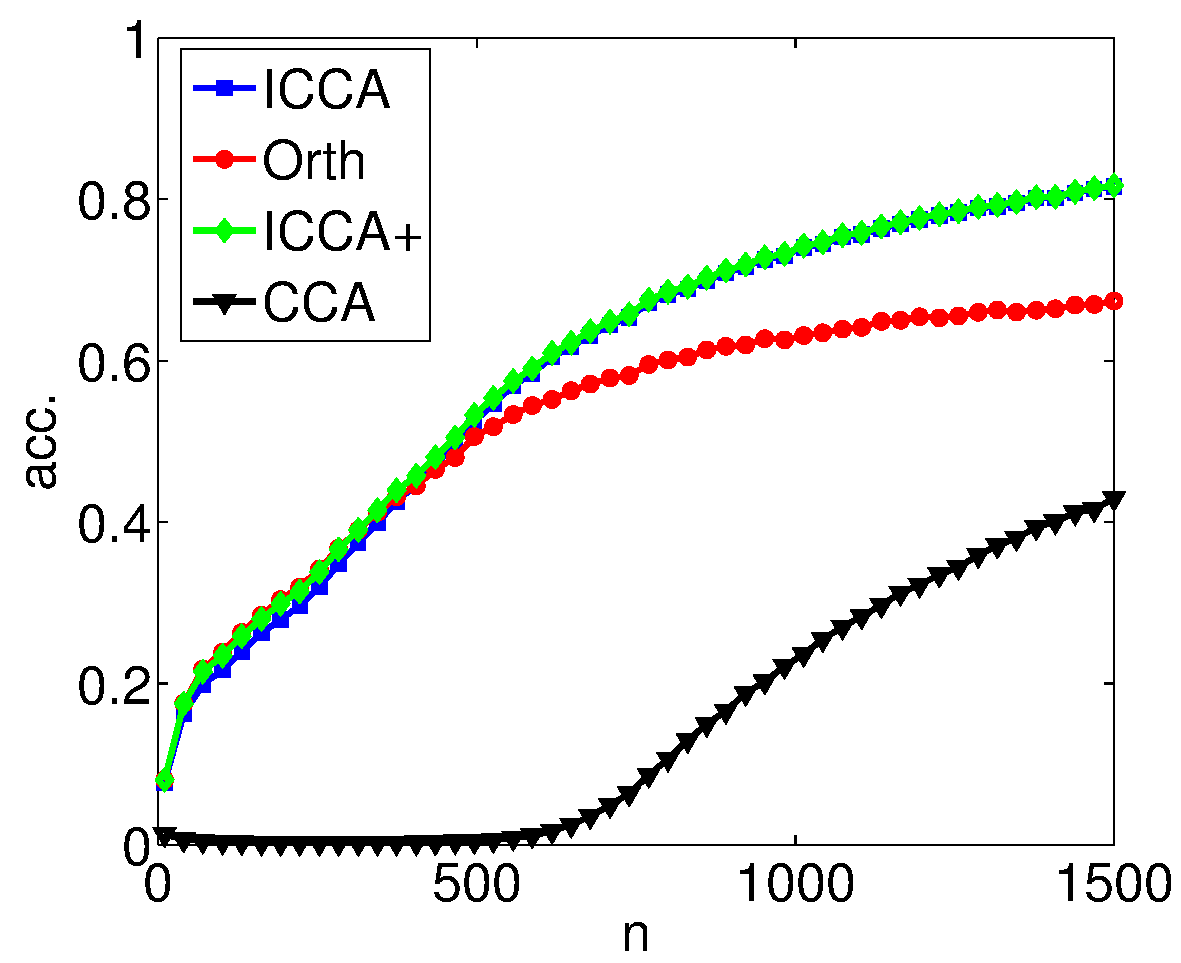
\includegraphics[width=0.47\textwidth]{chpt5_icca_vect/figs/icca_vect_n1.pdf}
    }
    \subfigure[$w_x^{(2)}$]{
      \label{fig:chpt5:non_ident2}
      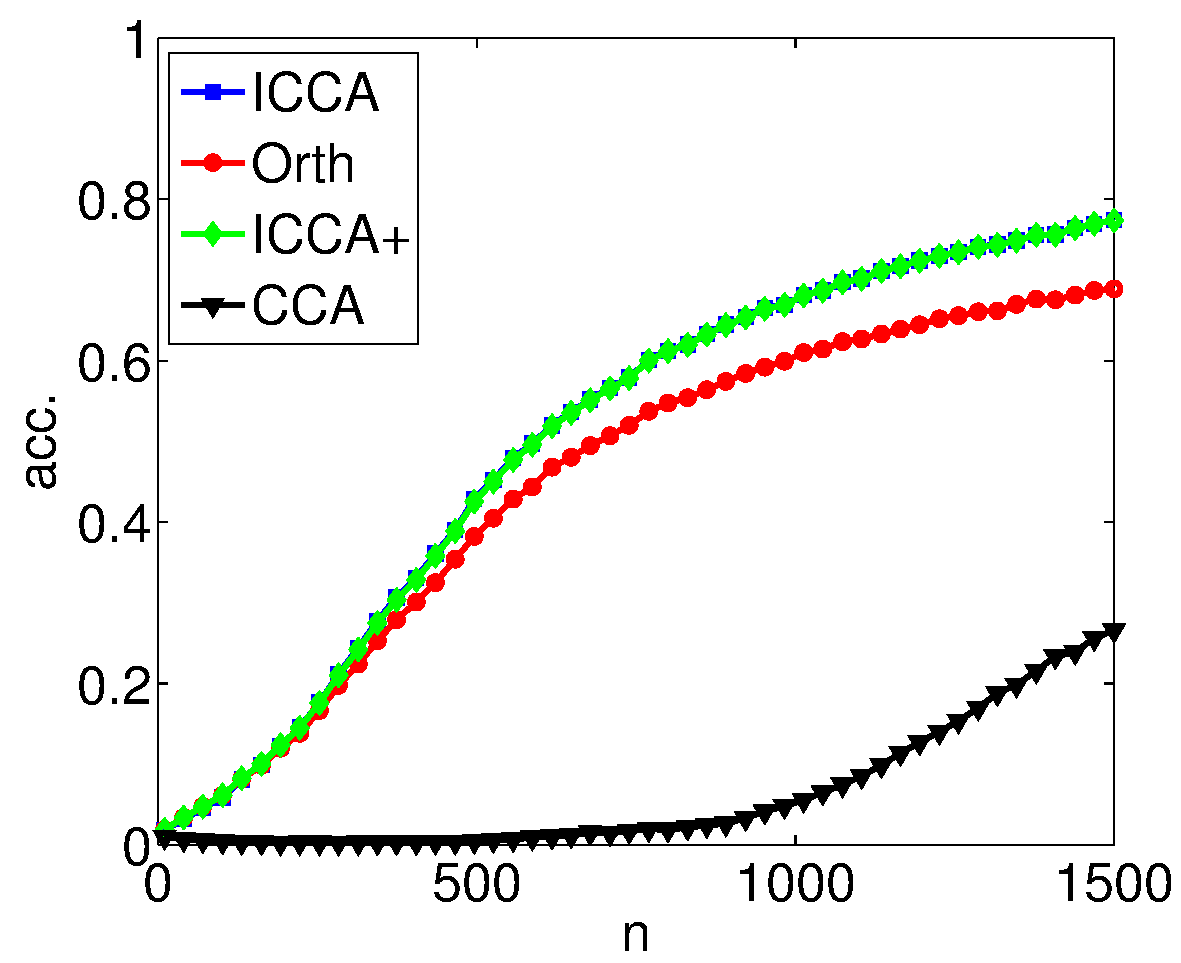
\includegraphics[width=0.47\textwidth]{chpt5_icca_vect/figs/icca_vect_n2.pdf}
    }
    \caption{Accuracy plots as a function of $n$ for a rank-2 setting where $\kx=\ky=2$,
      $p=200$, $q=250$, $\Tx=\Ty=\diag(16,1)$, $\Pxy=\diag(0.9,0.9)$, $V_K=I_2$, and
      non-identity $U_K$. Accuracy is defined in (\ref{eq:chpt5:cca_vect_acc}). The left
      figure plots the accuracy of the first canonical vector and the right figure plots
      the accuracy of the second canonical vector.}
    \label{fig:chpt5:non_ident_uktil}
  \end{center}
\end{figure}

\subsection{Convergence}

The theorems presented in this chapter state their results for the asymptotic regime of
$p,q,n\to\infty$ with $p/n\to c_x$ and $q/n\to c_y$. Here, for three fixed values of $c_x=0.5,
1, 2$, we generate data from (\ref{eq:chpt5:data_model}) with the parameters from Figure
\ref{fig:chpt5:non_ident_uktil} for 3 values of $p=100,500,1000$ to ensure that the estimates do
indeed converge. Figure \ref{fig:chpt5:icca_convg_w1} plots the accuracy as defined in
(\ref{eq:chpt5:cca_vect_acc}) for the first canonical vector for all four estimators. We also plot
one standard deviation errorbars from the simulation. Figures \ref{fig:chpt5:icca_vect_convg1}
and \ref{fig:chpt5:icca_vect_convg2} plot the accuracy convergence for the individual estimates
for both the first and second canonical vectors.

These three figures paint a nice picture of the different estimators. We first see that
the CCA estimator fails for all three values of $c_x$. This gives credence to Conjecture
\ref{conj:icca_vect} that when $n< p+q$ the canonical vectors returned by empirical CCA
are random. For the other three estimators, we see accuracy increase as $c_x$
decreases. This makes sense as we expect our estimates to perform better given more
samples relative to the dimension size. Next we note that as $p$ increases, the errorbars
on all estimates decrease, empirically verifying the belief that the accuracy does indeed
have an asymptotic limit. Finally, we note that these figures reinforce the fact that the
optimal weights are optimal in the asymptotic regime. For small $p$, the orthogonal
estimate slightly outperforms the \iccap estimate. However, when $p=1000$, we see that
this gap closes and that the \iccap estimate starts to outperform all other estimates.

\begin{figure}
  \begin{center}
    \subfigure[$p=100$]{
      \label{fig:chpt5:convg_p1}
      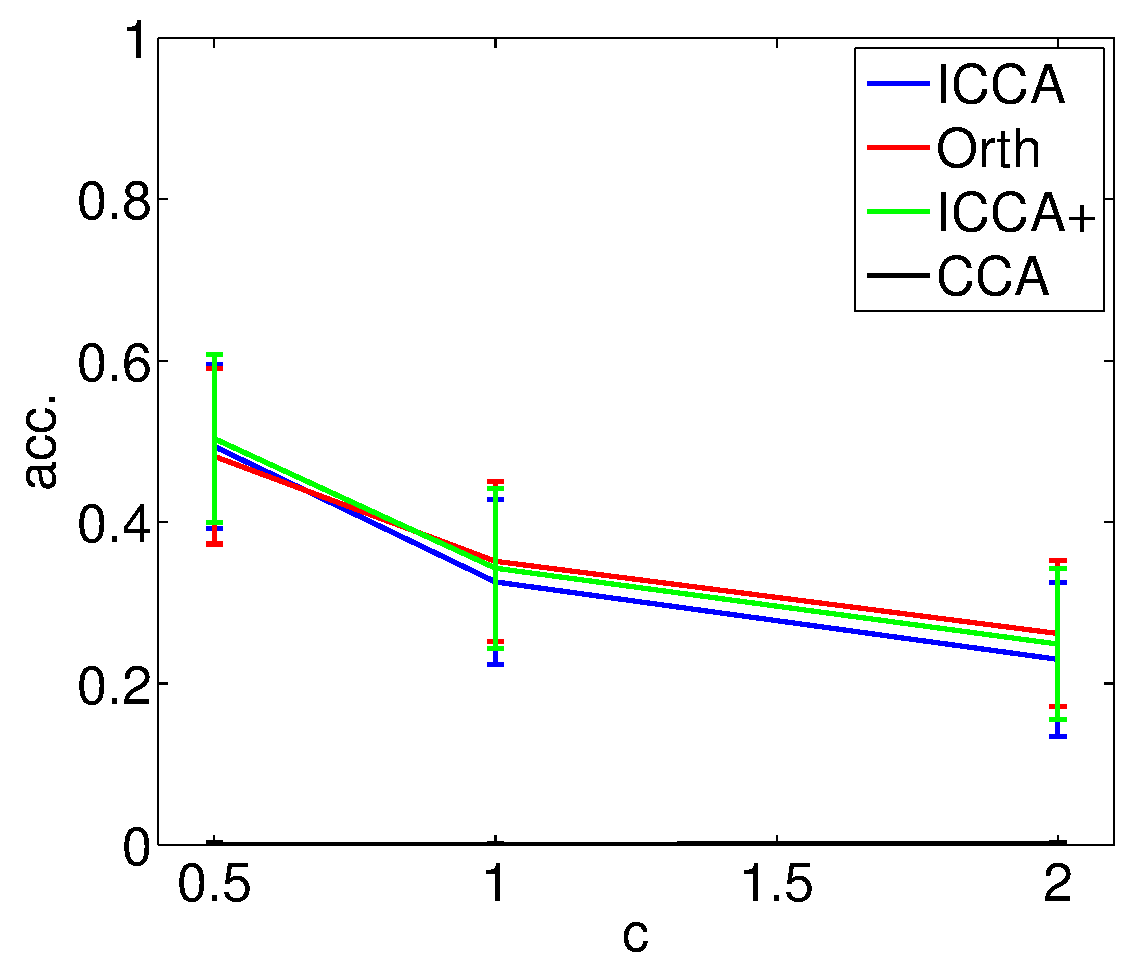
\includegraphics[width=0.3\textwidth]{chpt5_icca_vect/figs/icca_vect_convg_p1.pdf}
    }
    \subfigure[$p=500$]{
      \label{fig:chpt5:convg_p2}
      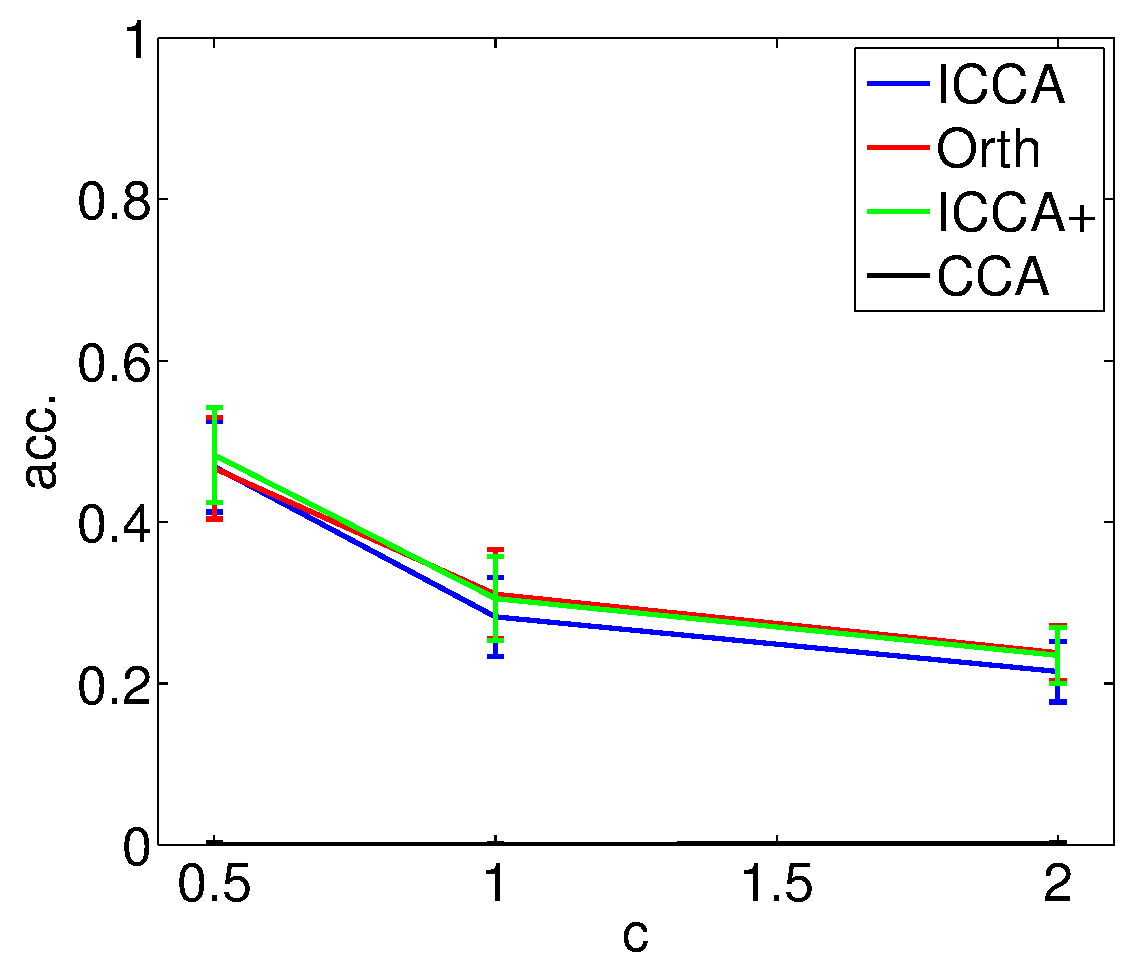
\includegraphics[width=0.3\textwidth]{chpt5_icca_vect/figs/icca_vect_convg_p2.pdf}
    }
    \subfigure[$p=1000$]{
      \label{fig:chpt5:convg_p3}
      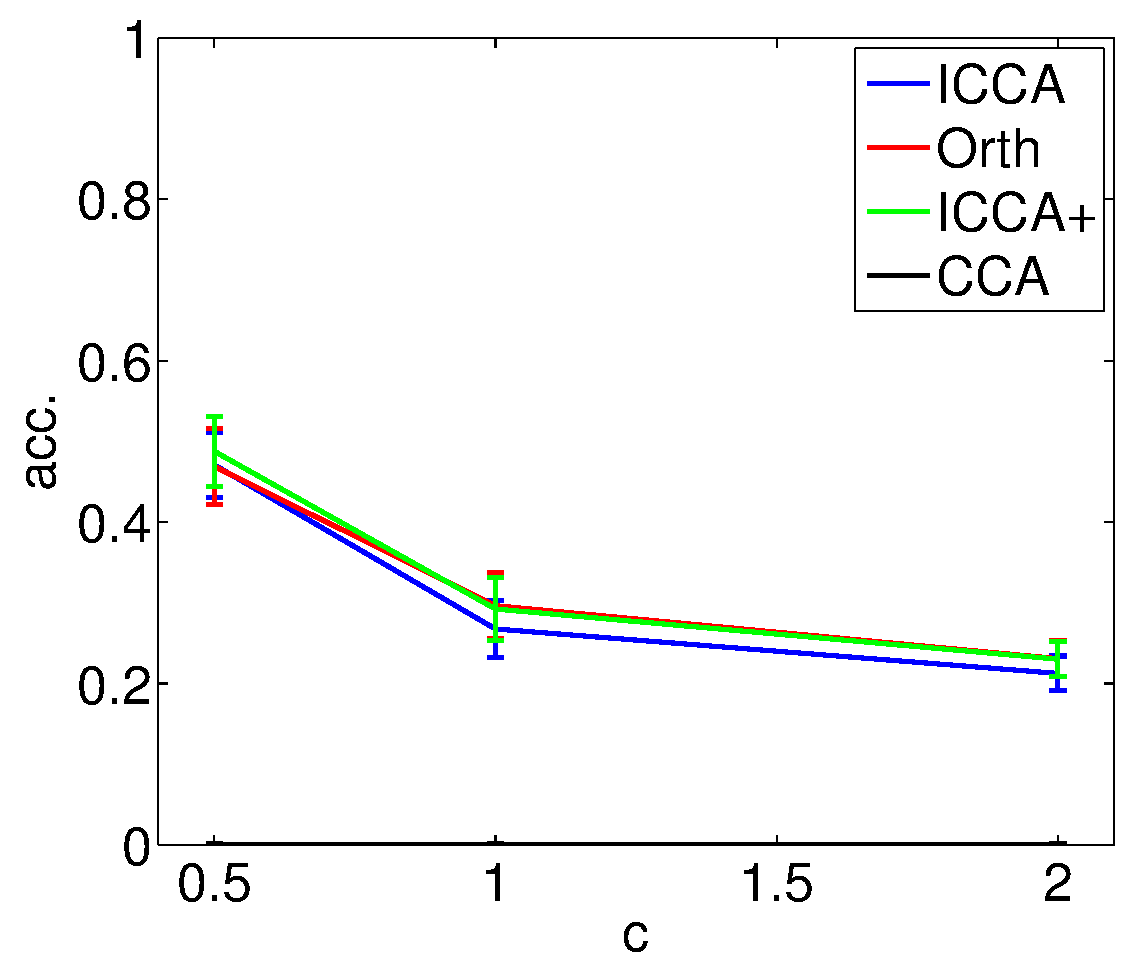
\includegraphics[width=0.3\textwidth]{chpt5_icca_vect/figs/icca_vect_convg_p3.pdf}
    }
    \caption{Convergence plots of the first canonical vector of each estimate for three
      values of $p$. Results are plotted for three fixed values of $c_x=0.5,1,2$. The
      simulation setting is the same as Figure \ref{fig:chpt5:non_ident_uktil} for a
      rank-2 setting where $\kx=\ky=2$, $p=200$, $q=250$, $\Tx=\Ty=\diag(16,1)$,
      $\Pxy=\diag(0.9,0.9)$, $V_K=I_2$, and non-identity $U_K$. Errorbars are 1 standard deviation.}
    \label{fig:chpt5:icca_convg_w1}
  \end{center}
\end{figure}


\begin{figure}
  \begin{center}
    \subfigure[ICCA $w_x^{(1)}$]{
      \label{fig:chpt5:convg_plugin1}
      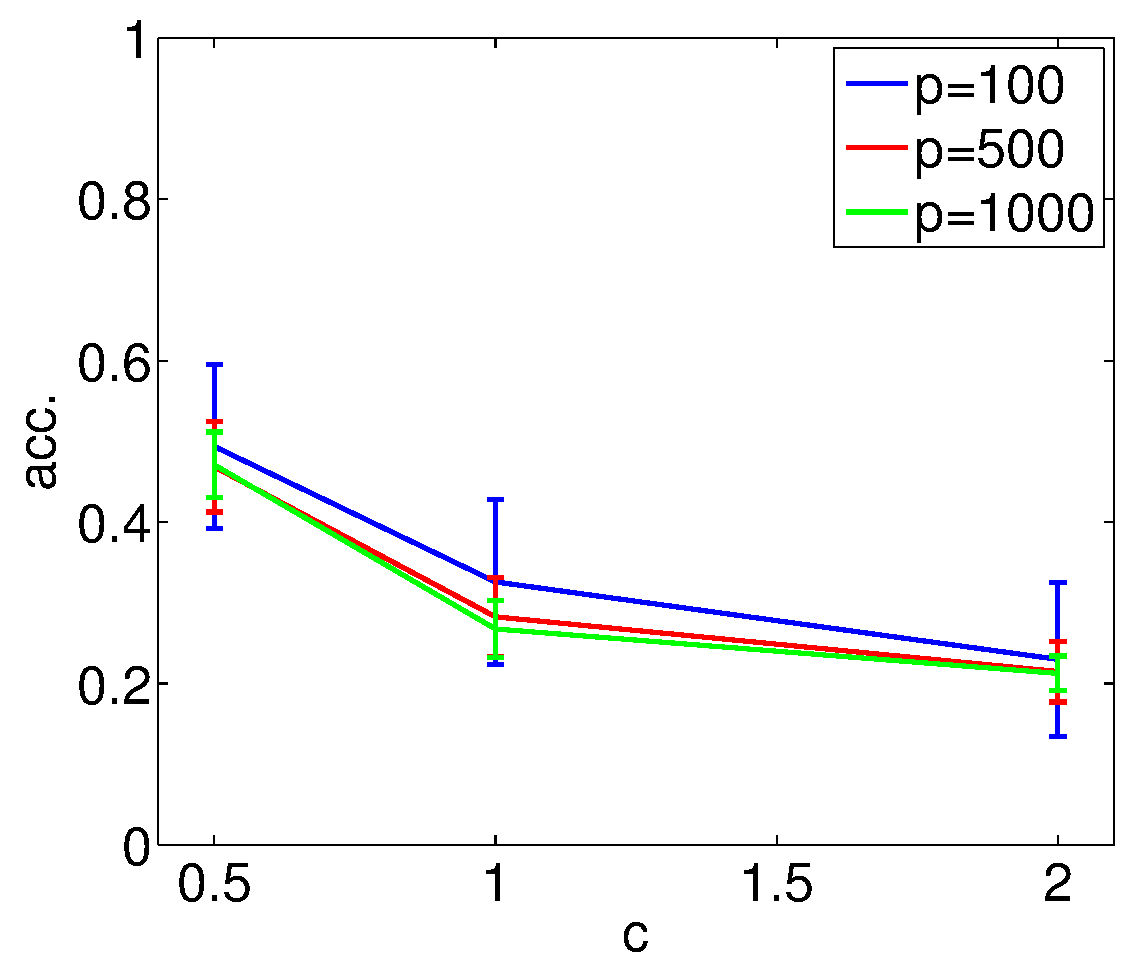
\includegraphics[width=0.47\textwidth]{chpt5_icca_vect/figs/icca_vect_convg_plugin_1.pdf}
    }
    \subfigure[ICCA $w_x^{(2)}$]{
      \label{fig:chpt5:convg_plugin2}
      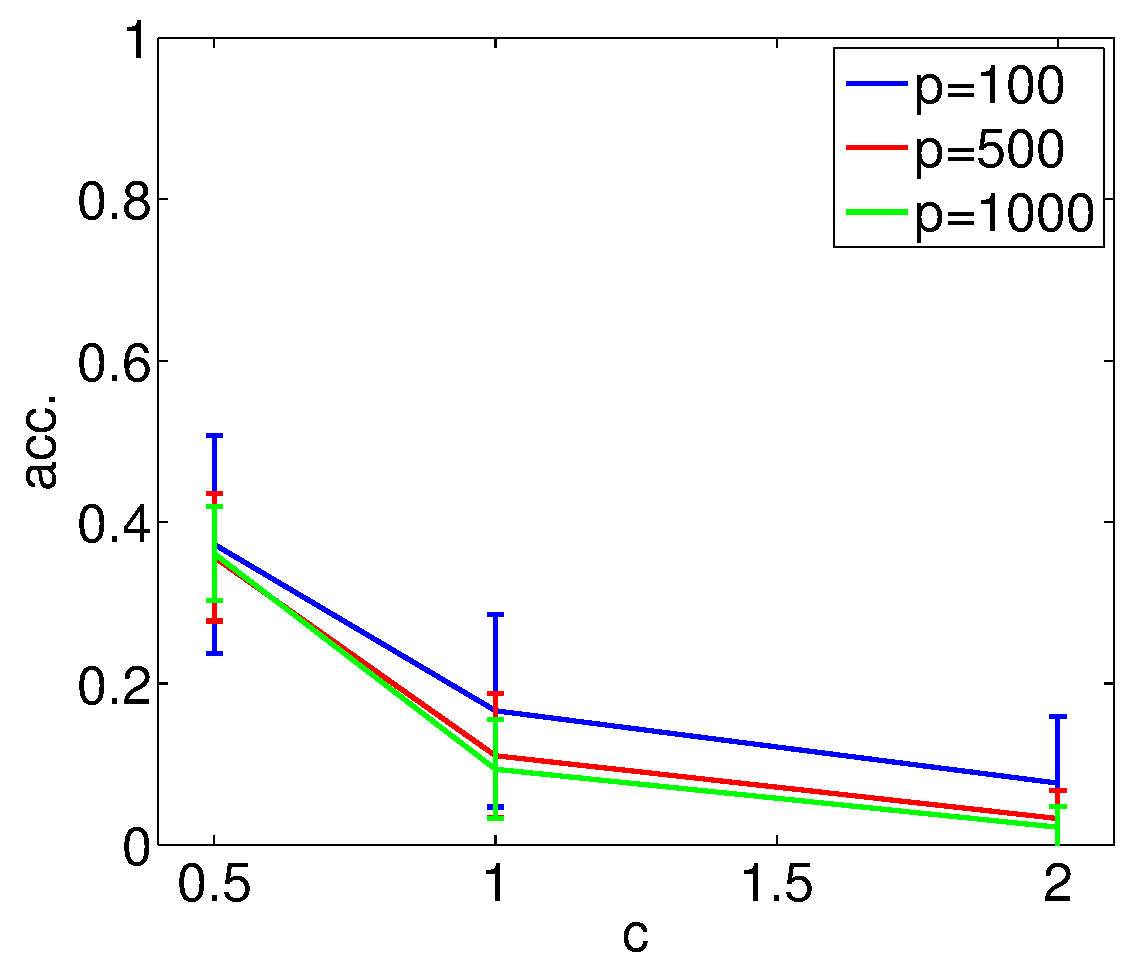
\includegraphics[width=0.47\textwidth]{chpt5_icca_vect/figs/icca_vect_convg_plugin_2.pdf}
    }
    \subfigure[\iccap $w_x^{(1)}$]{
      \label{fig:chpt5:convg_opt1}
      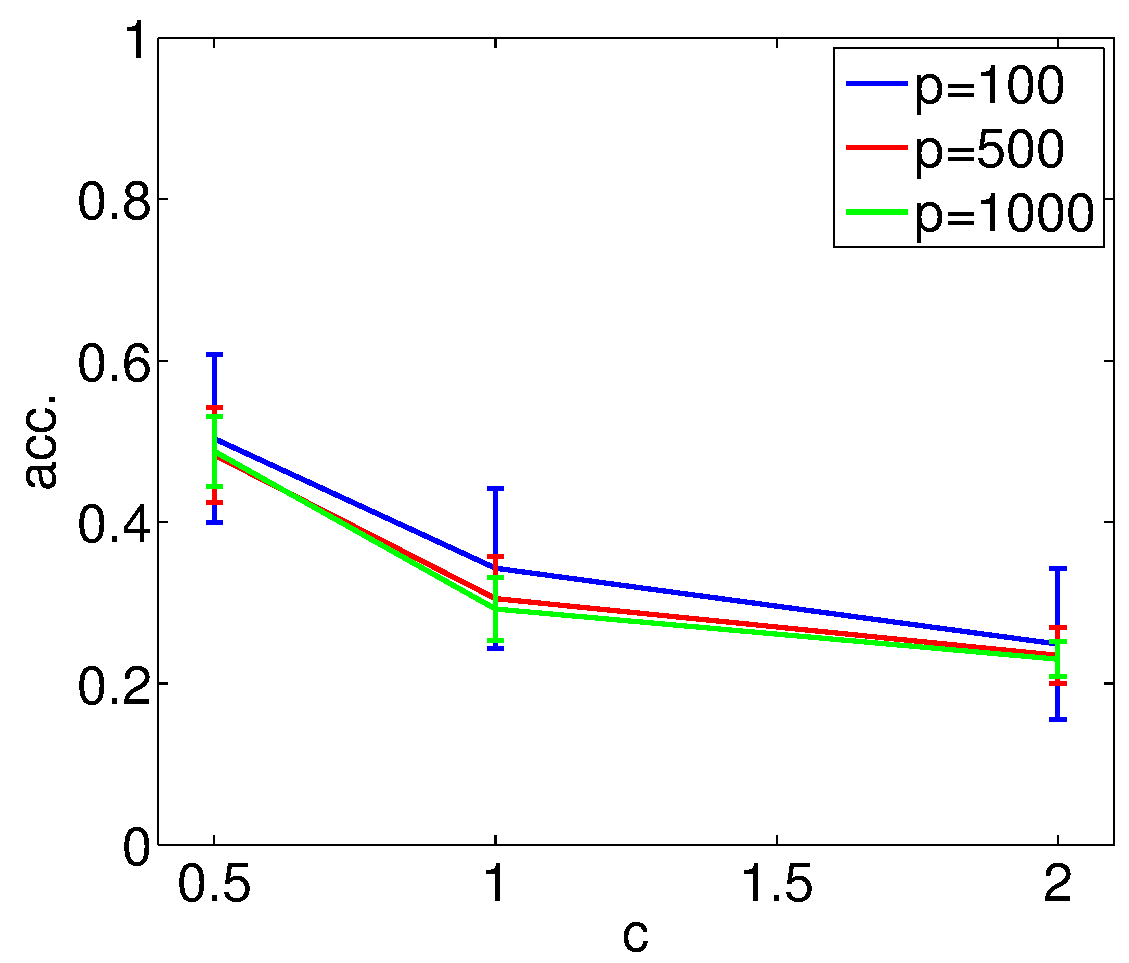
\includegraphics[width=0.47\textwidth]{chpt5_icca_vect/figs/icca_vect_convg_opt_1.pdf}
    }
    \subfigure[\iccap $w_x^{(2)}$]{
      \label{fig:chpt5:convg_opt2}
      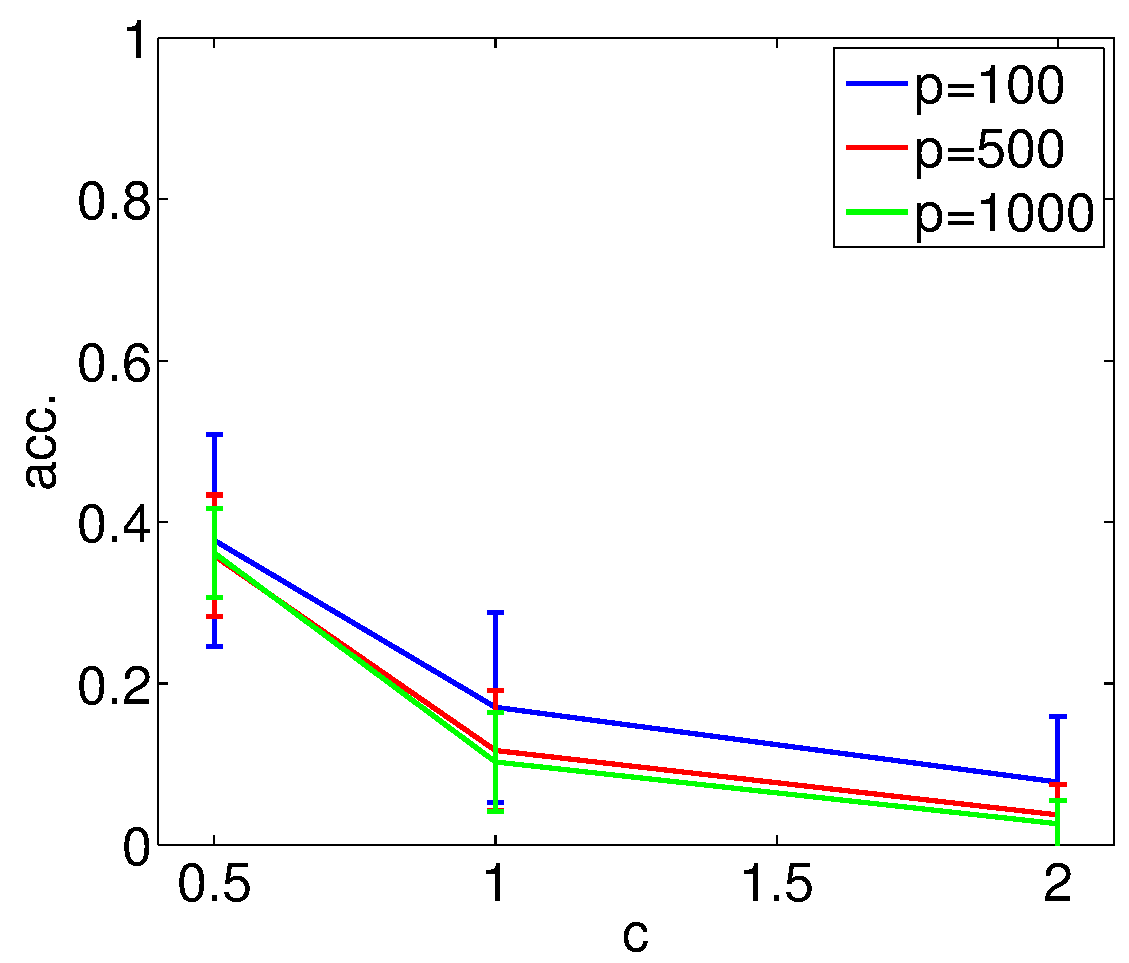
\includegraphics[width=0.47\textwidth]{chpt5_icca_vect/figs/icca_vect_convg_opt_2.pdf}
    }
    \caption{Accuracy convergence plots for the top two canonical vectors of the ICCA
      and \iccap estimates. Results are plotted for three fixed values of $c_x=0.5,1,2$
      for three different values of $p$. The simulation setting is the same as Figure
      \ref{fig:chpt5:icca_convg_w1} for a rank-2 setting where $\kx=\ky=2$, $p=200$,
      $q=250$, $\Tx=\Ty=\diag(16,1)$, $\Pxy=\diag(0.9,0.9)$, $V_K=I_2$, and non-identity
      $U_K$. Errorbars are 1 standard deviation.}
    \label{fig:chpt5:icca_vect_convg1}
  \end{center}
\end{figure}
\begin{figure}
  \begin{center}
    \subfigure[Orthogonal $w_x^{(1)}$]{
      \label{fig:chpt5:convg_orth1}
      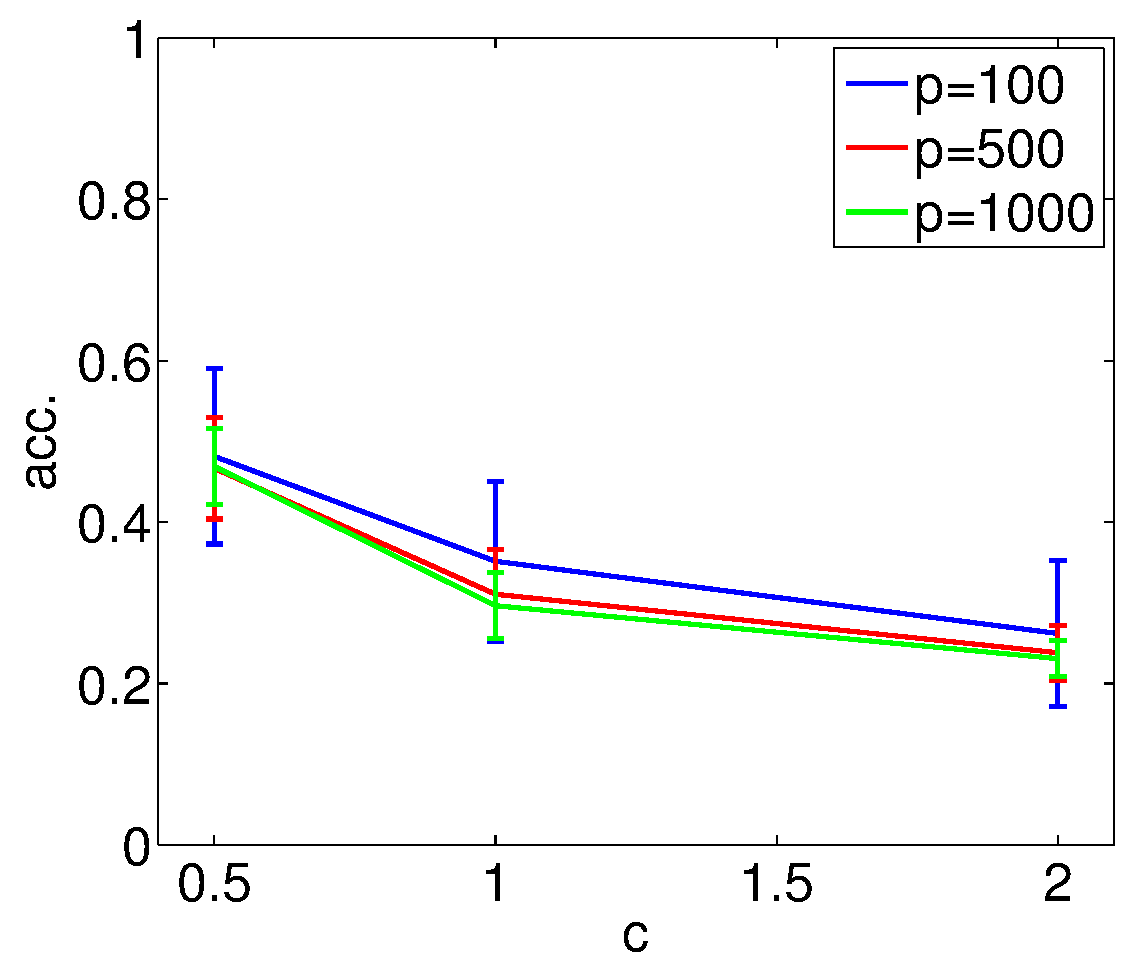
\includegraphics[width=0.47\textwidth]{chpt5_icca_vect/figs/icca_vect_convg_orth_1.pdf}
    }
    \subfigure[Orthogonal $w_x^{(2)}$]{
      \label{fig:chpt5:convg_orth2}
      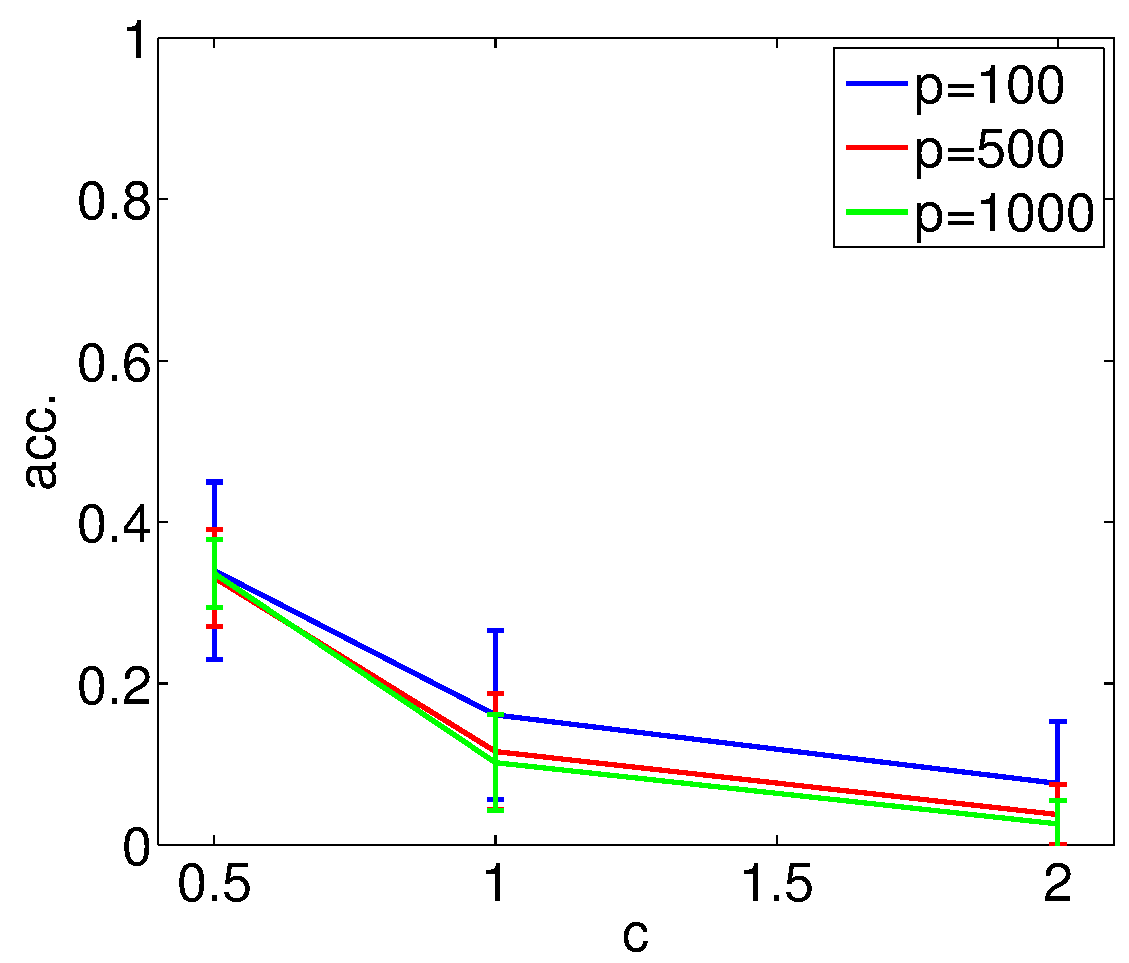
\includegraphics[width=0.47\textwidth]{chpt5_icca_vect/figs/icca_vect_convg_orth_2.pdf}
    }
    \subfigure[Empirical CCA $w_x^{(1)}$]{
      \label{fig:chpt5:convg_cca1}
      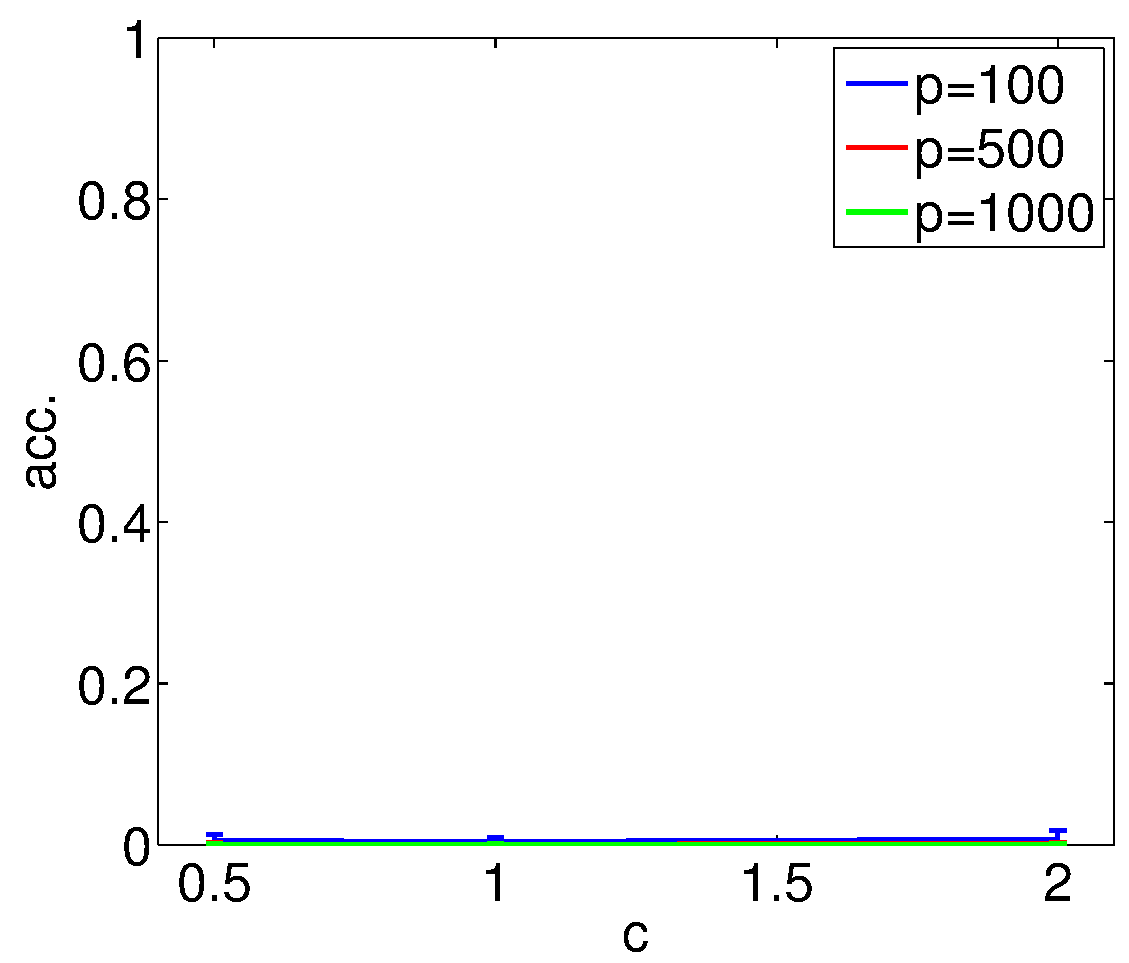
\includegraphics[width=0.47\textwidth]{chpt5_icca_vect/figs/icca_vect_convg_cca_1.pdf}
    }
    \subfigure[Empirical CCA $w_x^{(2)}$]{
      \label{fig:chpt5:convg_cca2}
      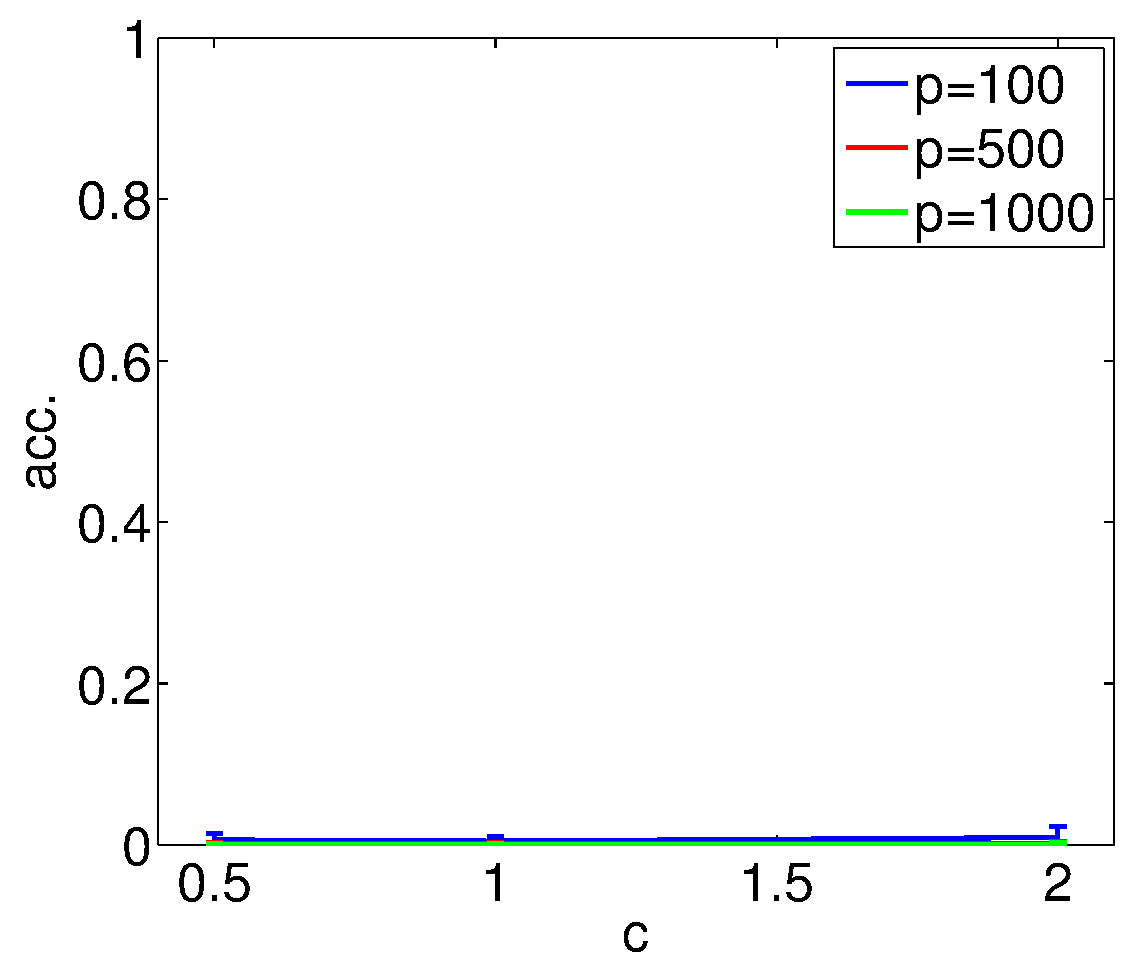
\includegraphics[width=0.47\textwidth]{chpt5_icca_vect/figs/icca_vect_convg_cca_2.pdf}
    }
    \caption{Accuracy convergence plots for the top two canonical vectors of the
      orthogonal and empirical CCA estimates. Results are plotted for three fixed values
      of $c_x=0.5,1,2$ for three different values of $p$. The simulation setting is the
      same as Figure \ref{fig:chpt5:icca_convg_w1} for a rank-2 setting where $\kx=\ky=2$,
      $p=200$, $q=250$, $\Tx=\Ty=\diag(16,1)$, $\Pxy=\diag(0.9,0.9)$, $V_K=I_2$, and
      non-identity $U_K$. Errorbars are 1 standard deviation.}
    \label{fig:chpt5:icca_vect_convg2}
  \end{center}
\end{figure}


\subsection{Robustness to $\kxhat$}

Finally we explore the performance of our estimators when we change the estimate of the
number of subspace components, $\kxhat$. The theorems presented in this chapter assume
that $\kxhat=\kx$. However, we explore the performance of these estimates when this
assumption is not valid. Figure \ref{fig:chpt5:khat_c1} and \ref{fig:chpt5:khat_c2} plot
the performance of the estimates while sweeping over $\kxhat=\kyhat$ for $c_x=0.2$ and
$c_x=1$, respectively. We use a different simulation setting than Figure
\ref{fig:chpt5:non_ident_uktil}. Here we set setting $\kx=\ky=3$, $p=200$, $q=250$,
$\Tx=\Ty=\diag(3,2,1)$, $\Pxy=\diag(0.9,0.5,0.3)$,$V_k=I_3$ and 
\be
U_k= \left[\frac{1}{\sqrt{3}}\left[\begin{array}{c} 1\\ 1\\1\end{array}\right],
    \frac{1}{\sqrt{2}}\left[\begin{array}{c} 1\\
        0\\-1\end{array}\right],\frac{1}{\sqrt{6}}\left[\begin{array}{c} 1\\
        -2\\1\end{array}\right]\right]. 
\ee

From these Figures we see that all estimates suffer greatly when $\kxhat<\kx=3$. This
makes sense as we don't use all of the possible signals that are present. The more
interesting behavior occurs when we overestimate $\kx$, which is a common practice in many
applications.  We see that the first canonical vector in both cases remains robust to
overestimating $\kxhat$. This first canonical vector corresponds to the largest singular
value of $\Kxytil$ and so the corresponding singular vector estimate is accurate. However,
the higher order canonical vectors are less accurate as we overestimate $\kxhat$. This
accuracy suffers more for $w_x^{(3)}$ with increasing $\kxhat$. For the case of $c=0.2$ in
Figure \ref{fig:chpt5:khat_c1}, we see that for these parameters, \iccap is the most robust
even as we greatly overestimate $\kxhat$ and that the orthogonal estimate is more accurate
than the ICCA estimate when we overestimate $\kxhat$. This makes sense as $\Tx$ and $\Ty$
are very close to identity. For all cases though, the CCA estimate is very bad and all of
the ICCA, orthogonal, and \iccap estimates greatly outperform it. In Figure
\ref{fig:chpt5:khat_c2} when $c=1$, we see that the accuracy is much lower for all
estimates; this makes sense as a larger $c$ corresponds to fewer samples. Still though,
the \iccap estimate is the most robust estimate and the CCA estimate is completely random.

\begin{figure}
  \begin{center}
    \subfigure[$w_x^{(1)}$]{
      \label{fig:chpt5:khat11}
      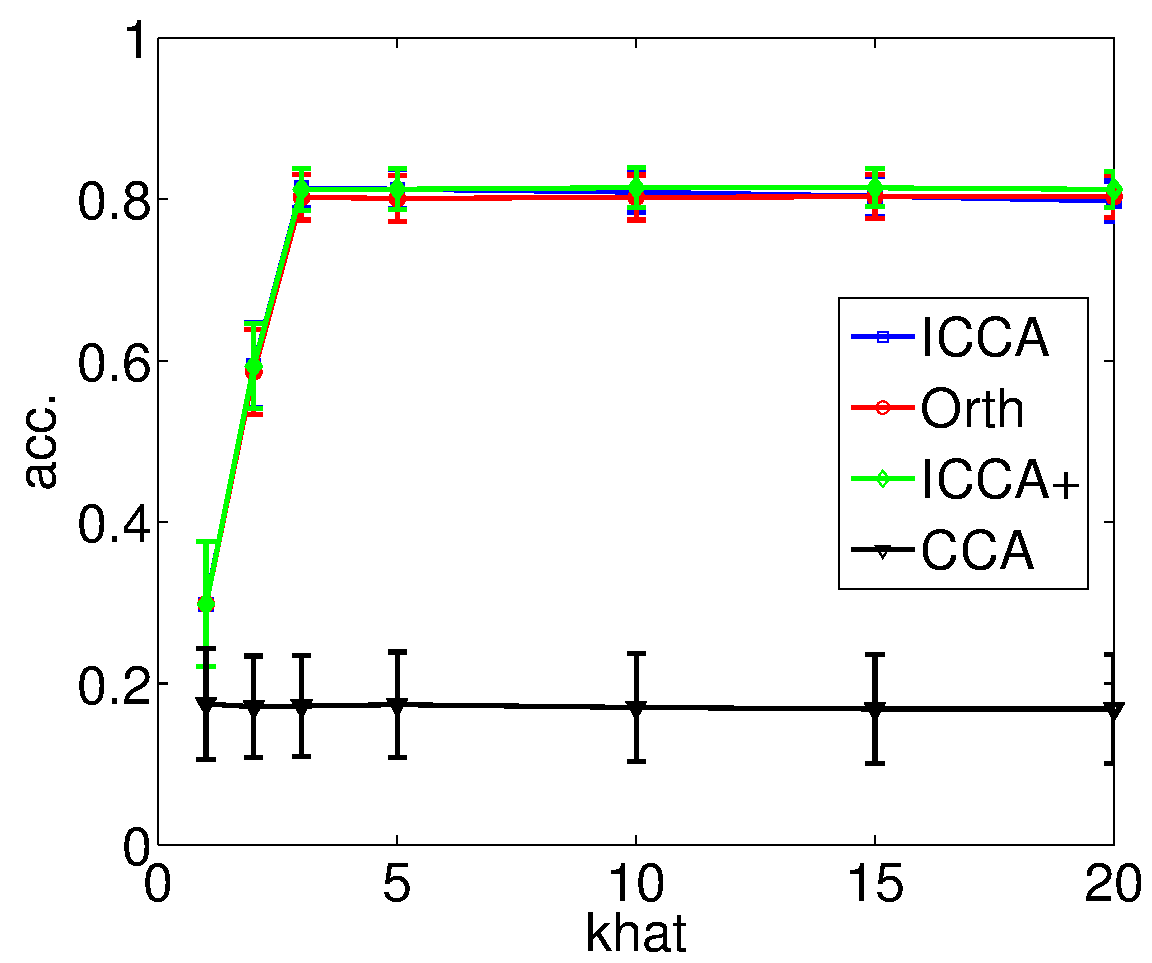
\includegraphics[width=0.45\textwidth]{chpt5_icca_vect/figs/icca_vect_khat1_1.pdf}
    }
    \subfigure[$w_x^{(2)}$]{
      \label{fig:chpt5:khat13}
      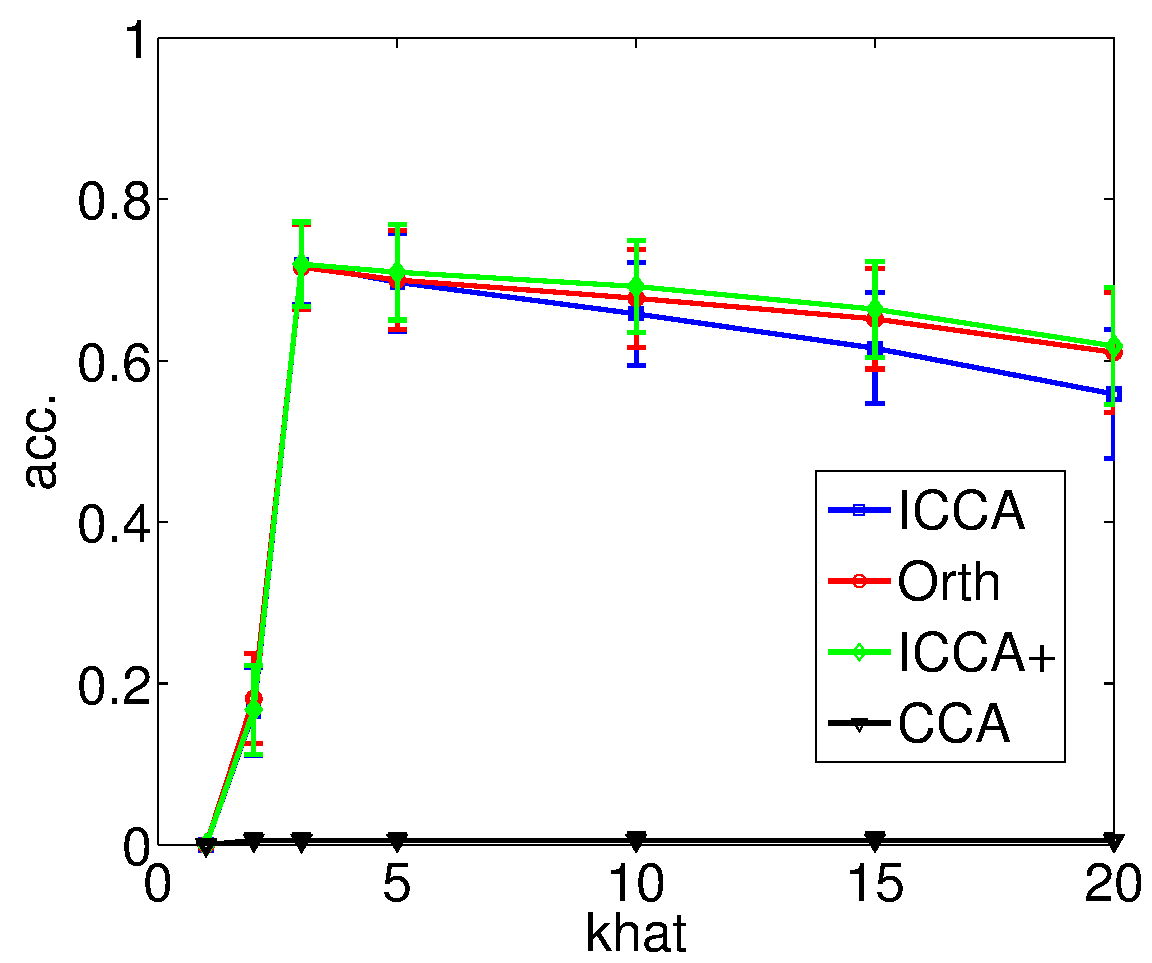
\includegraphics[width=0.45\textwidth]{chpt5_icca_vect/figs/icca_vect_khat1_2.pdf}
    }
    \subfigure[$w_x^{(3)}$]{
      \label{fig:chpt5:khat13}
      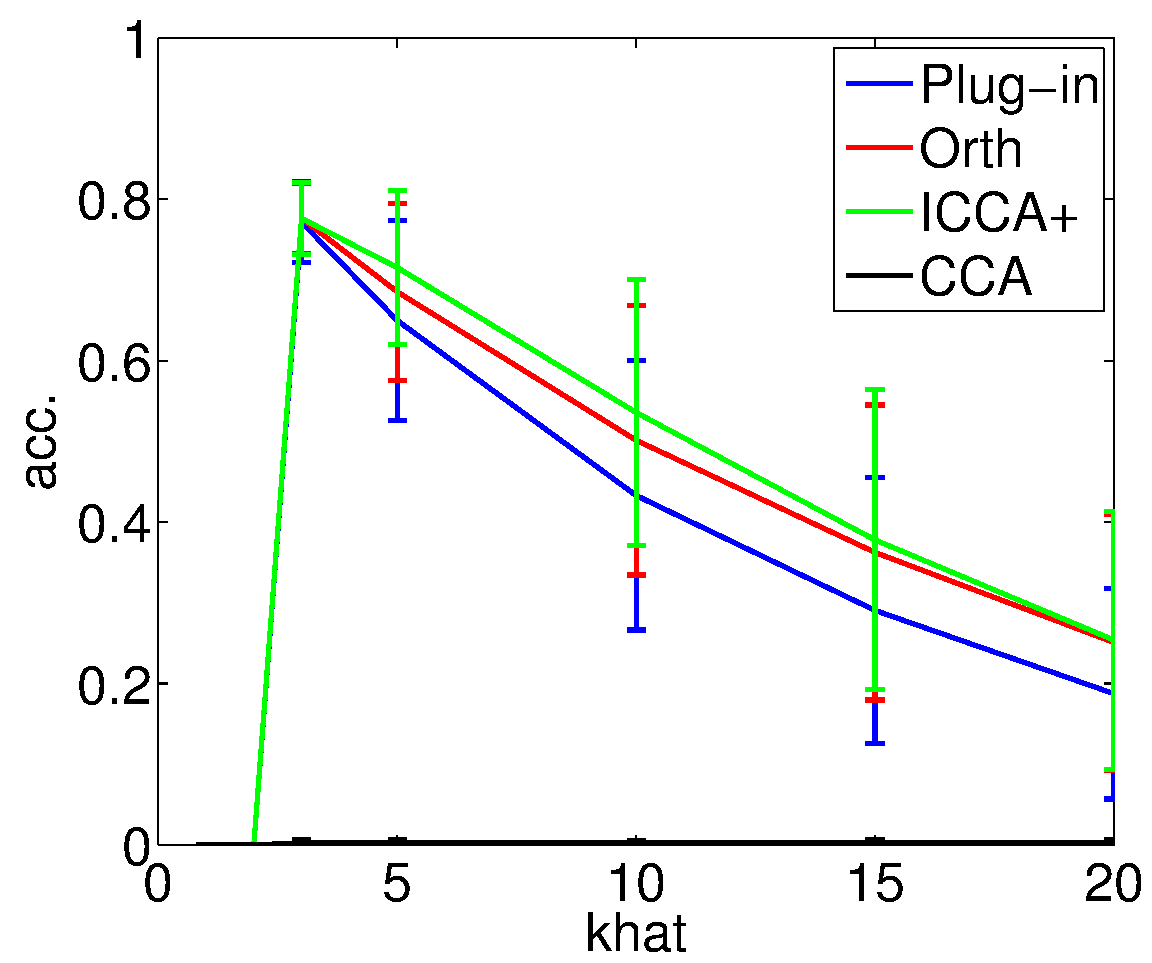
\includegraphics[width=0.45\textwidth]{chpt5_icca_vect/figs/icca_vect_khat1_3.pdf}
    }
    \caption{Accuracy plots of the first two canonical vector estimates a function of
      $\kxhat$ for $c=0.2$. The simulation setting is the same as Figure
      \ref{fig:chpt5:icca_convg_w1} for a rank-2 setting where $\kx=\ky=2$, $p=200$,
      $q=250$, $\Tx=\Ty=\diag(16,1)$, $\Pxy=\diag(0.9,0.9)$, $V_K=I_2$, and non-identity
      $U_K$. Errorbars are 1 standard deviation.}
    \label{fig:chpt5:khat_c1}
  \end{center}
\end{figure}

\begin{figure}
  \begin{center}
    \subfigure[$w_x^{(1)}$]{
      \label{fig:chpt5:khat21}
      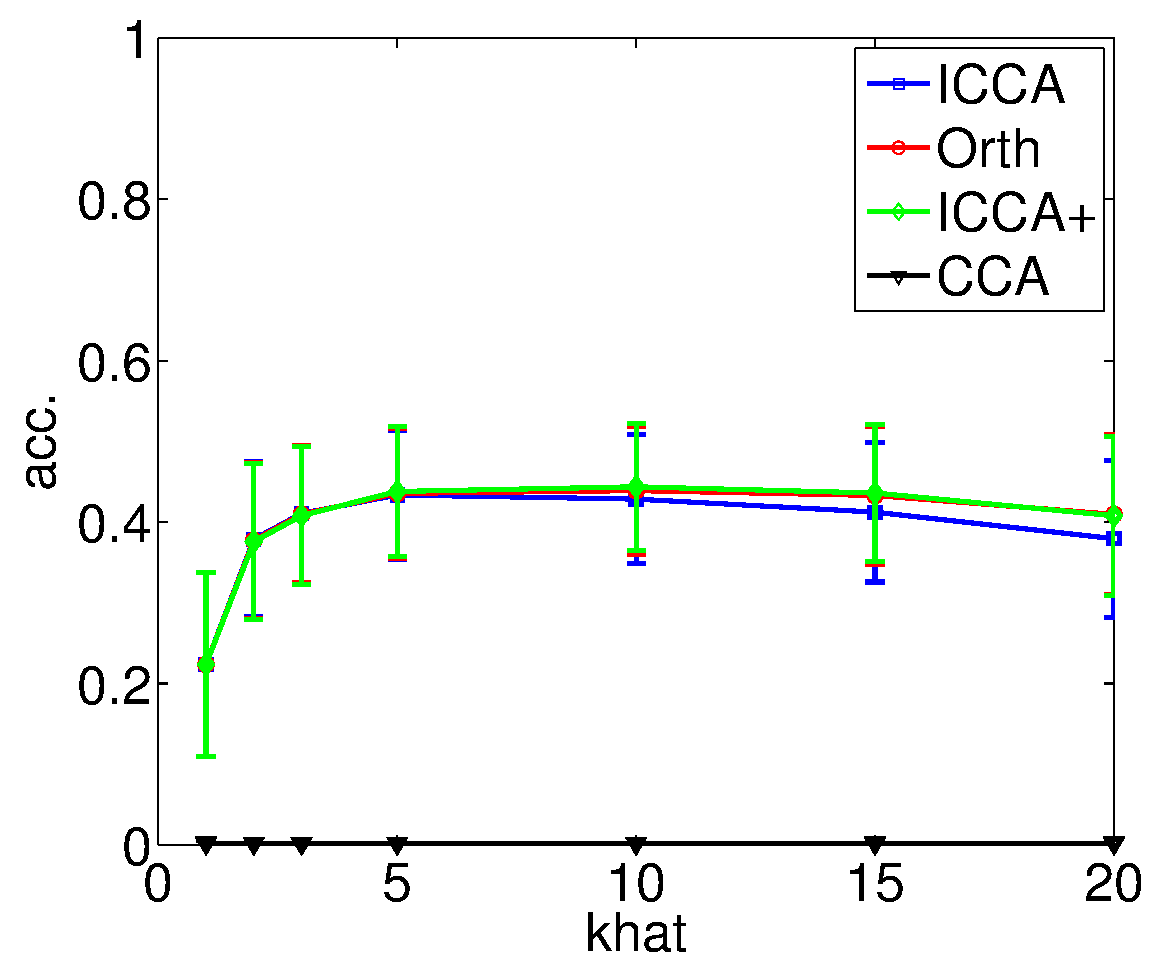
\includegraphics[width=0.45\textwidth]{chpt5_icca_vect/figs/icca_vect_khat2_1.pdf}
    }
    \subfigure[$w_x^{(2)}$]{
      \label{fig:chpt5:khat22}
      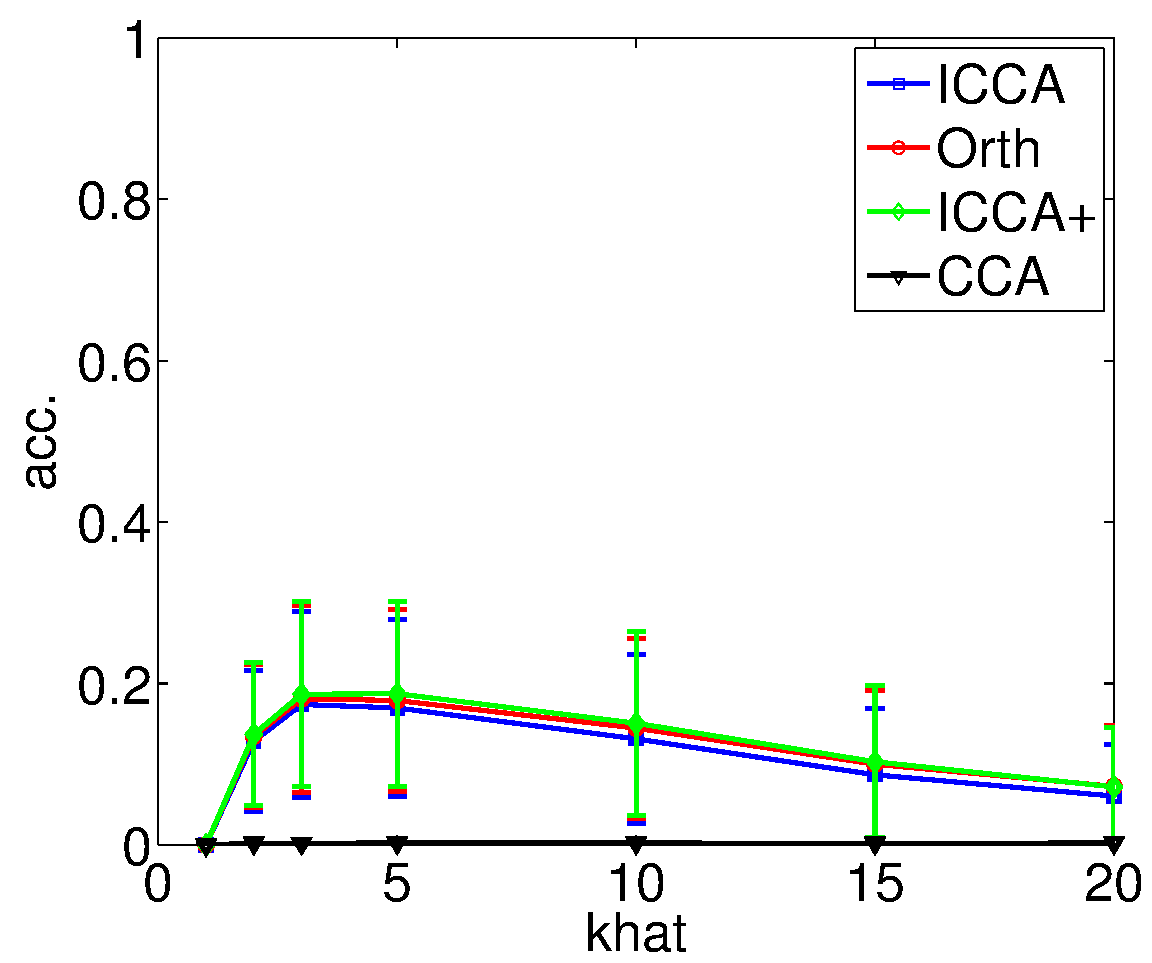
\includegraphics[width=0.45\textwidth]{chpt5_icca_vect/figs/icca_vect_khat2_2.pdf}
    }
    \subfigure[$w_x^{(3)}$]{
      \label{fig:chpt5:khat23}
      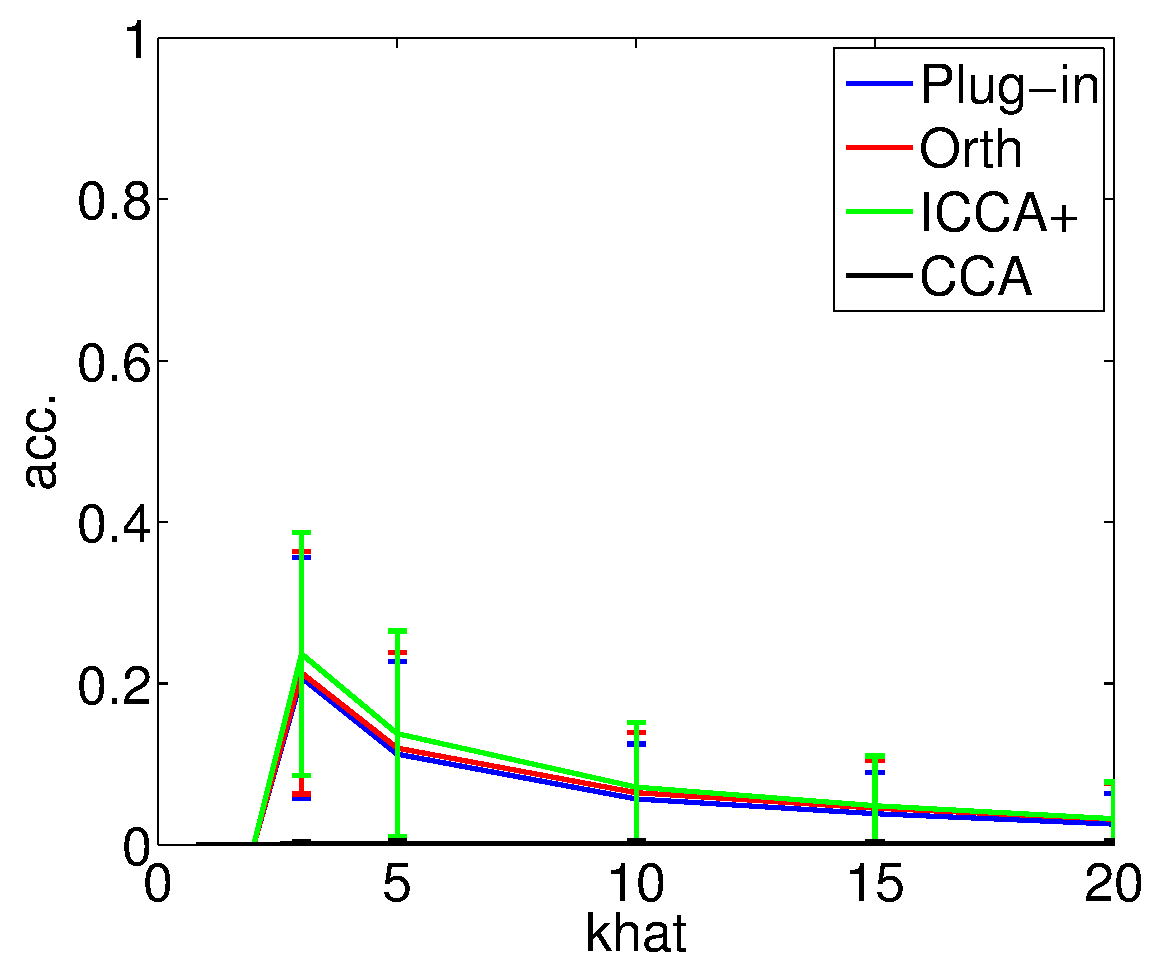
\includegraphics[width=0.45\textwidth]{chpt5_icca_vect/figs/icca_vect_khat2_3.pdf}
    }
    \caption{Accuracy plots of the first two canonical vector estimates a function of
      $\kxhat$ for $c=1$. The simulation setting is the same as Figure
      \ref{fig:chpt5:icca_convg_w1} for a rank-2 setting where $\kx=\ky=2$, $p=200$,
      $q=250$, $\Tx=\Ty=\diag(16,1)$, $\Pxy=\diag(0.9,0.9)$, $V_K=I_2$, and non-identity
      $U_K$. Errorbars are 1 standard deviation.}
    \label{fig:chpt5:khat_c2}
  \end{center}
\end{figure}

\section{Empirical Results - Real-World Data}

To compare the performance of these canonical vector estimates on real world applications,
we reuse two of the controlled experiments we created in Chapter
\ref{sec:chpt_cca_det}. These examples showcase quite well the very nuanced behavior of
the ICCA, orthogonal, and \iccap estimates. We recall that the \iccap estimate is
optimal in an asymptotic sense and so that, as in some of these examples, finite $p,q,n$
cause the \iccap estimates to perform slightly worse than the ICCA or orthogonal
estimates. The ICCA canonical vector estimate requires the inversion of $\Rxxhat$ and
$\Ryyhat$ (or equivalently computing the SVD of $X$ and $Y$), which involves inverting the
estimated singular values of $\Rxx$ and $\Ryy$. In some cases, inaccurate singular value
estimates actually improve the weightings applied to the singular vectors, which thus
improves the canonical vector accuracy. While the orthogonal estimate works quite well
when $\Uktil$ is identity, it suffers a performance loss when this assumption is not
true. Therefore, even in the finite $p,q,n$ applications, the \iccap canonical vector
estimate is the most robust estimator. 

\subsection{Video-Video Experiment}

First, we use the video-video experiment consisting of 5 stationary flashing lights and
two stationary iPhone cameras. Figure \ref{fig:chpt5:flashing_sources} shows the views
from the left and right cameras and manually identifies each source. The 5 sources are a
blue flashing police light (BPL) outlined in the green rectangle, one phone with a
flashing strobe light (PH1) outlined in the dark blue rectangle, another phone with a
flashing strobe light (PH2) outlined in a red rectangle, a tablet with a flashing screen
(T1) outlined in the magenta rectangle, and a red flashing police light (RPL) outlined in
the cyan rectangle. From left to right, the left camera can see BPL, PH1, and PH2. From
left to right, the right camera can see PH2, T1, and RPL. Therefore, both cameras share
the common signal of PH2. As we saw in Chapter \ref{sec:chpt_cca_det}, the police lights
RPL and BPL are in antiphase and thus also correlated. Therefore, for this experiment each
view has 3 signals, two of which are correlated. 

\begin{figure}
  \begin{center}
    \subfigure[Left Camera]{
      \label{fig:chpt5:flashing_left}
      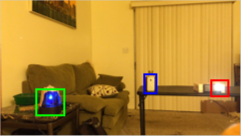
\includegraphics[width=0.47\textwidth]{chpt5_icca_vect/figs/flashing_left_sources.png}
    }
    \subfigure[Right Camera]{
      \label{fig:chpt5:flashing_right}
      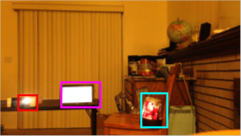
\includegraphics[width=0.47\textwidth]{chpt5_icca_vect/figs/flashing_right_sources.png}
    }   
    \caption{Manual source identification of each camera. Both cameras share a common
      flashing phone, outlined in a red rectangle. Each camera has two independent sources
      besides the shared flashing phone.}
    \label{fig:chpt5:flashing_sources}
  \end{center}
\end{figure}

To synchronize the cameras we used the RecoLive MultiCam iPhone app
\footnote{http://recolive.com/en/}. After turning on all light sources, we recorded 30
seconds of video at 30 frames per second. The resolutions of the iPhone's cameras were
both $1920\times 1080$ pixels. To post-process the video data, we first converted the
video streams to grayscale and then downsampled each spatial dimension by a factor of 8,
resulting in a resolution of $240\times 135$. We then vectorized each image and stacked
the 900 frames into data matrices , both of dimension $32400 \times 900$. Finally, we
subtract the mean from each dataset so that we may run PCA, CCA, and ICCA on the zero-mean
datasets, $X_{\text{left}}$ and $Y_{\text{right}}$. 

To run these algorithms, we use knowledge of the simulation setup and set
$\kxhat=\kyhat=3$. Figures \ref{fig:chpt5:flashing2_1} - \ref{fig:chpt5:flashing1_1} plot
the first canonical vector estimates for the left camera after frame 5, 30, and 600,
respectively. Each figure plots the absolute value of the ICCA, orthogonal, \iccaps, and
empirical CCA canonical vector estimates. We plot the absolute value or each vector to
discover correlated pixels; a left canonical vector gives more weight to left camera
pixels it believe are correlated with the pixels in the right camera. Each figure also
plots the difference between the ICCA and \iccap canonical vectors and the difference
between the orthogonal and \iccap canonical vectors. In these difference figures, pixels
with negative values represent pixels that the \iccap estimate believes are more
correlated while positive values represent pixels that the \iccap estimate believes
are less correlated. We plot the ICCA, orthogonal, and \iccap estimates on the same
scale, but plot the CCA estimates on its own scale because they vary widely (i.e. are
inaccurate). 

We can draw a number of conclusions from Figures \ref{fig:chpt5:flashing2_1} -
\ref{fig:chpt5:flashing1_1}. First, the empirical CCA canonical vector estimates are
meaningless. This gives credence to Conjecture \ref{conj:icca_vect} because we are in the
sample deficient regime where the number of pixels is much larger than the number of
frames that we have. Second, the first population canonical vector identifies the shared
camera PH2, which is the rightmost source in the left camera. As we get more frames, these
canonical vector estimates become more ``accurate'', i.e. identify only that
source. Third, the ICCA, orthogonal, and \iccap canonical vectors estimates are all very
similar. Each estimate places a large weight on pixels around the shared source,
PH2. However, there are slight differences between the estimates as seen in the
sub-figures (e) and (f). We note that the scale of these differences in on the order of
$10^{-3}$, which is fairly small compared to the magnitude of the pixels. First we see
that the ICCA estimate places more weight on the middle source PH1 than the \iccap
estimate. This is not desirable as source PH1 is not correlated with any source in the
right camera. Second, we see that the orthogonal estimate places less weight on source PH1
and less weight on source BPL than the \iccap estimate. This is desirable as these
sources are not correlated with the shared source PH2.

Therefore, we can conclude for this first canonical vector, the orthogonal estimate
performs the best and that the \iccap estimate performs better than the plug-in
estimate. We attribute this behavior to the fact that there is no mixing of principle
components in this example, as each source is identified as a principle component (see
Chapter \ref{sec:chpt_cca_det}). This results in a $\Uktil$ very close to identity, which
is when the orthogonal estimate is known to perform well.

\begin{figure}
  \begin{center}
    \subfigure[ICCA]{
      \label{fig:chpt5:flashing2_1_plugin}
      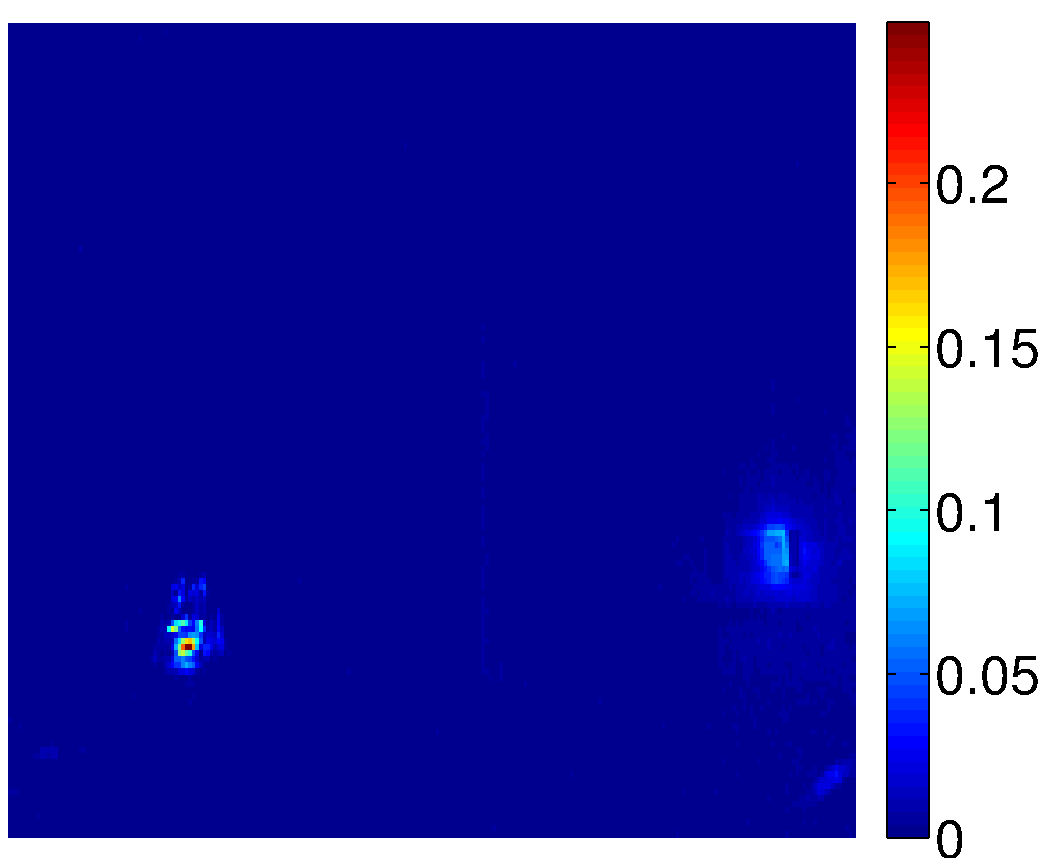
\includegraphics[width=0.45\textwidth]{chpt5_icca_vect/figs/flashing2_left1_icca.pdf}
    }
    \subfigure[Orthogonal]{
      \label{fig:chpt5:flashing2_1_orth}
      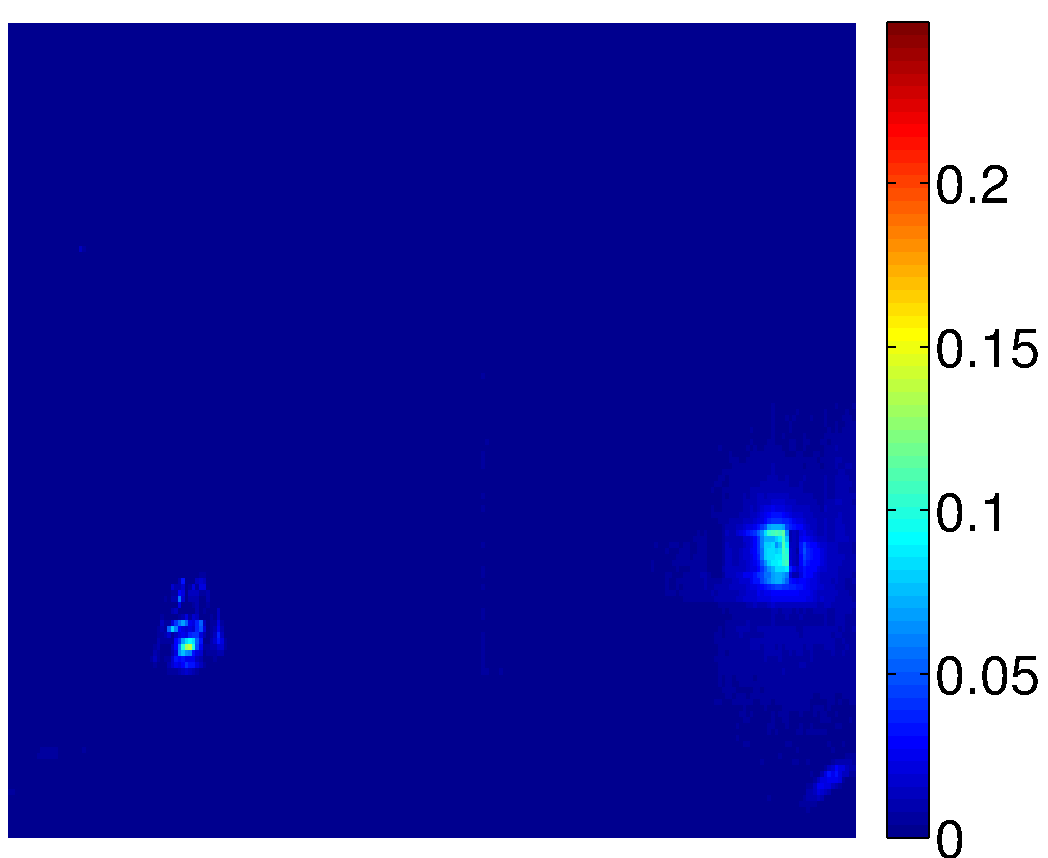
\includegraphics[width=0.45\textwidth]{chpt5_icca_vect/figs/flashing2_left1_orth.pdf}
    }
    \subfigure[\iccap]{
      \label{fig:chpt5:flashing2_1_opt}
      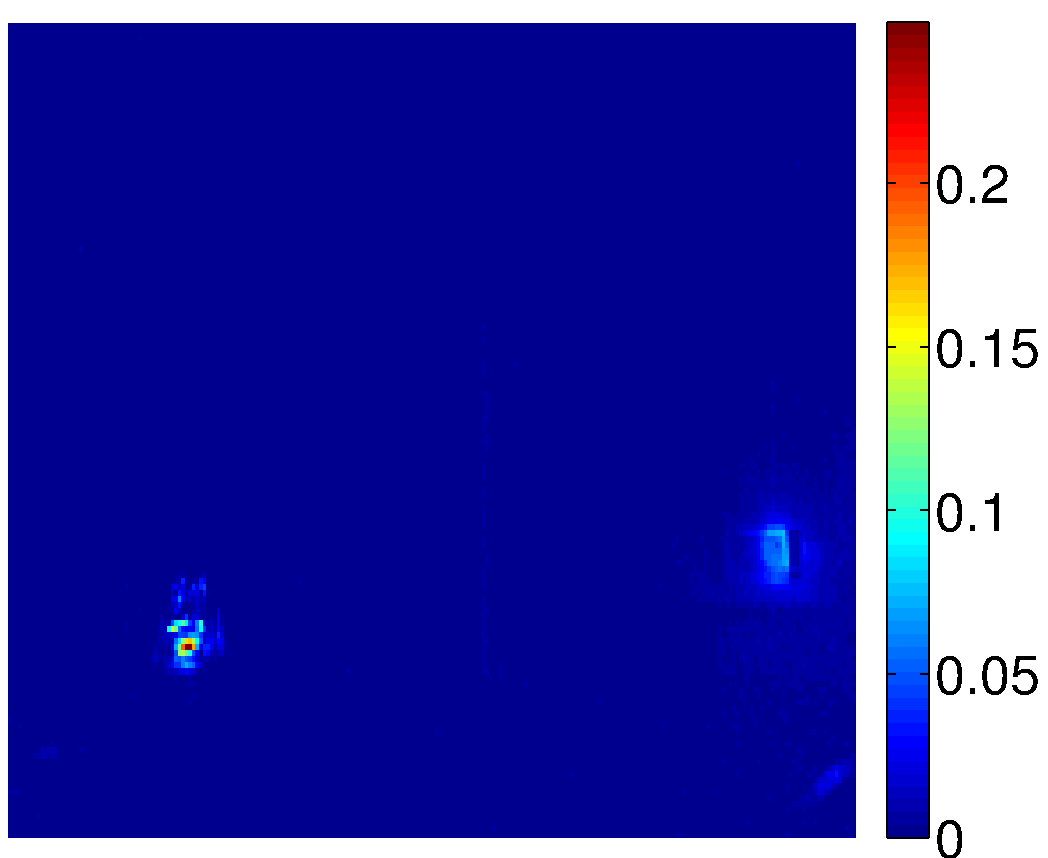
\includegraphics[width=0.45\textwidth]{chpt5_icca_vect/figs/flashing2_left1_opt.pdf}
    }
    \subfigure[CCA]{
      \label{fig:chpt5:flashing2_1_cca}
      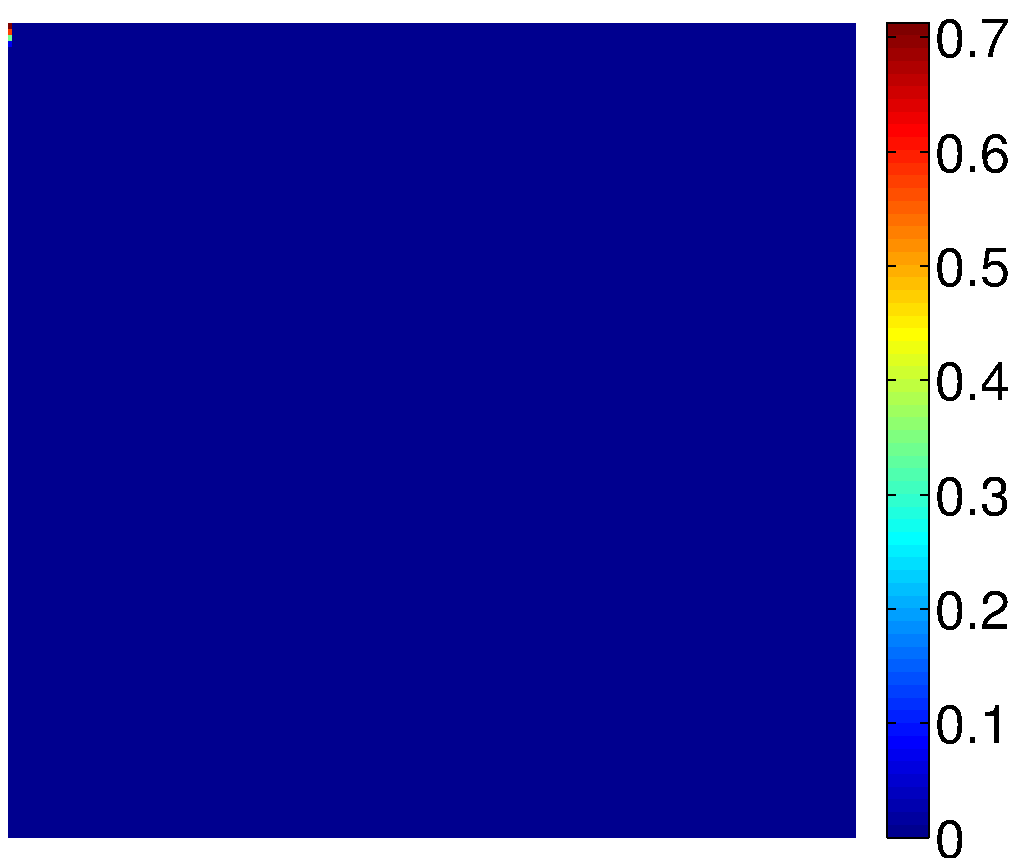
\includegraphics[width=0.45\textwidth]{chpt5_icca_vect/figs/flashing2_left1_cca.pdf}
    }
    \subfigure[ICCA minus \iccap]{
      \label{fig:chpt5:flashing2_1_diff1}
      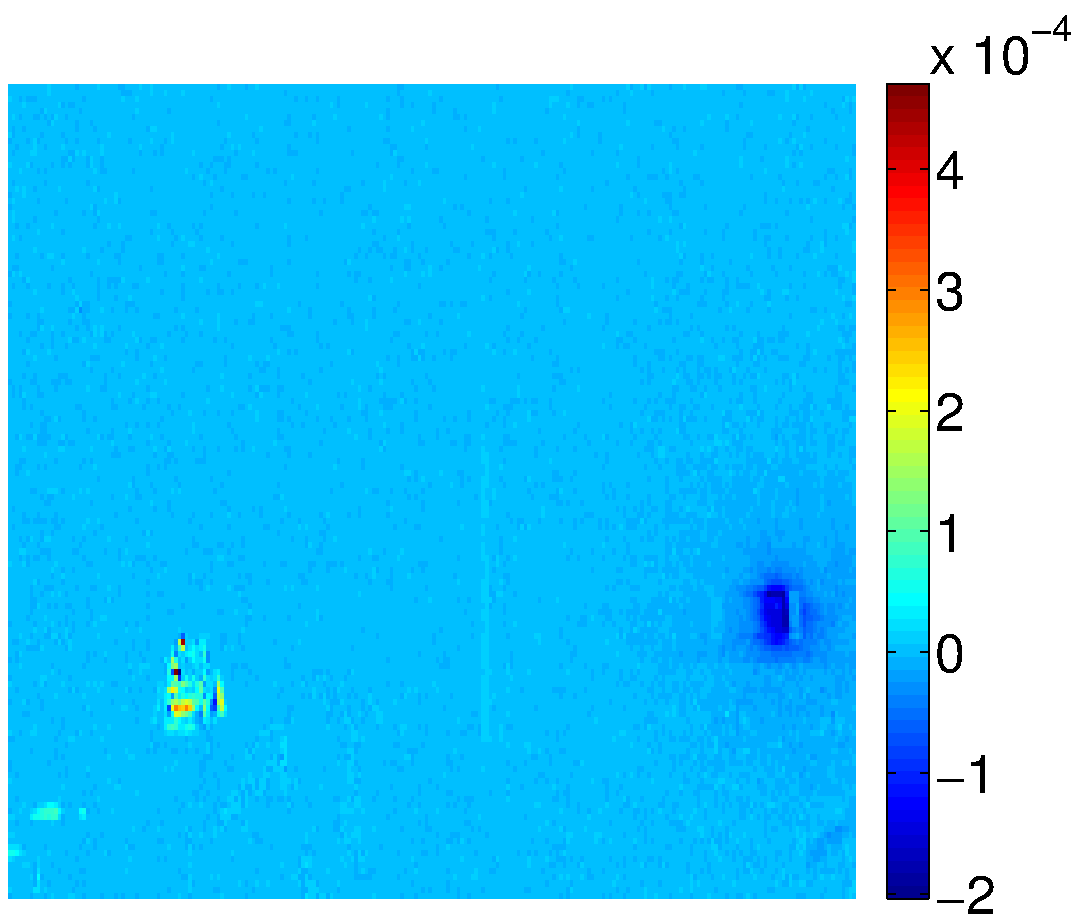
\includegraphics[width=0.45\textwidth]{chpt5_icca_vect/figs/flashing2_left1_diff_icca.pdf}
    }
    \subfigure[Orthogonal minus \iccap]{
      \label{fig:chpt5:flashing2_1_diff2}
      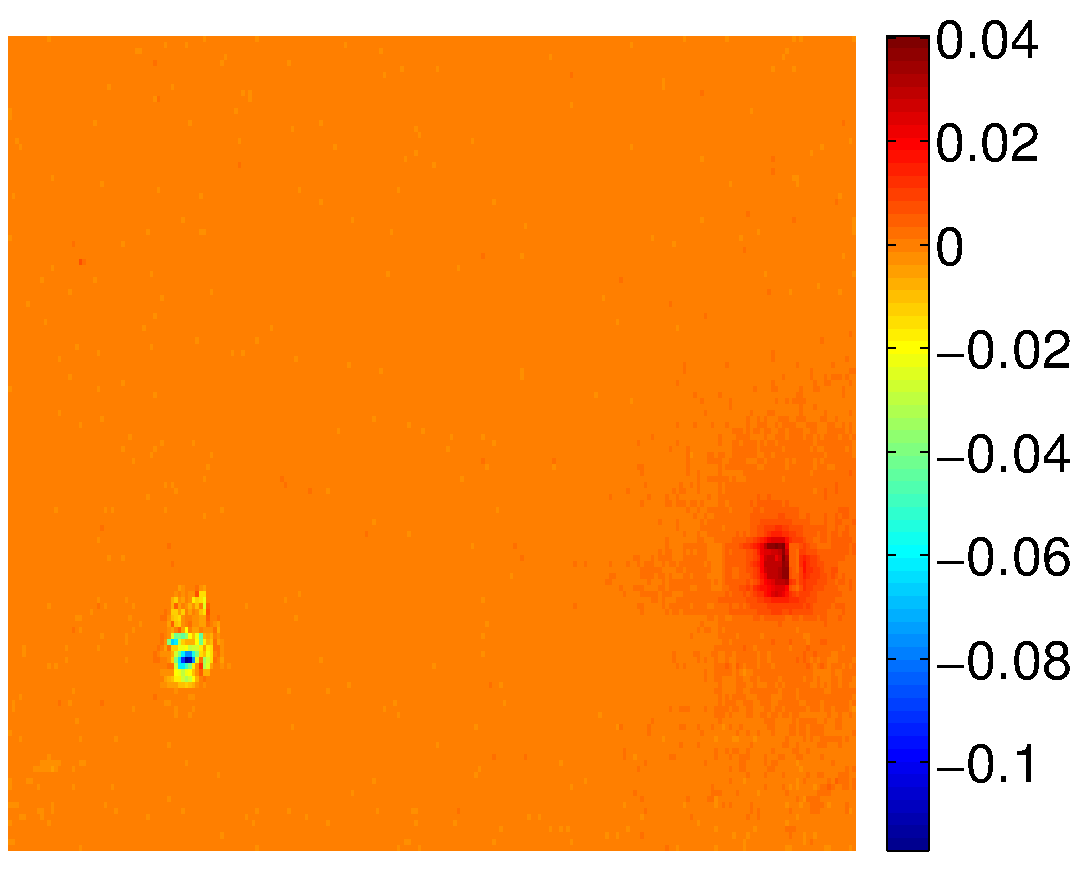
\includegraphics[width=0.45\textwidth]{chpt5_icca_vect/figs/flashing2_left1_diff_orth.pdf}
    }
    \caption{First canonical vector estimates for the left camera at frame 5. This corresponds
      to a total capture time of 1/6 of a second. (a)-(d) show the absolute value of the
      vectors displayed in an image so that large values indicate correlated
      pixels. (e)-(f) plot the difference between the ICCA estimate and the \iccap
      estimate and the orthogonal estimate and the \iccap estimate. Positive values
      indicate pixels that the \iccap estimate thinks are less correlated while negative
      values indicate pixels that the \iccap estimate thinks are more correlated. }
    \label{fig:chpt5:flashing2_1}
  \end{center}
\end{figure}

\begin{figure}
  \begin{center}
    \subfigure[ICCA]{
      \label{fig:chpt5:flashing3_1_plugin}
      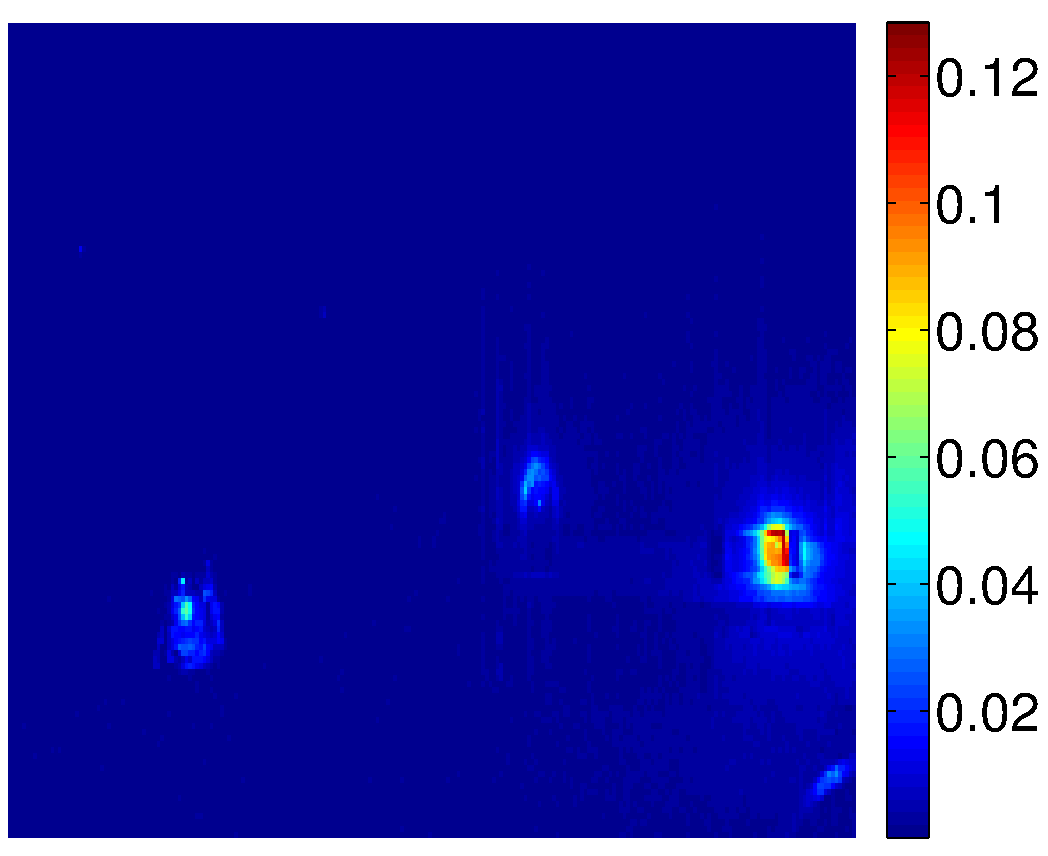
\includegraphics[width=0.45\textwidth]{chpt5_icca_vect/figs/flashing3_left1_icca.pdf}
    }
    \subfigure[Orthogonal]{
      \label{fig:chpt5:flashing3_1_orth}
      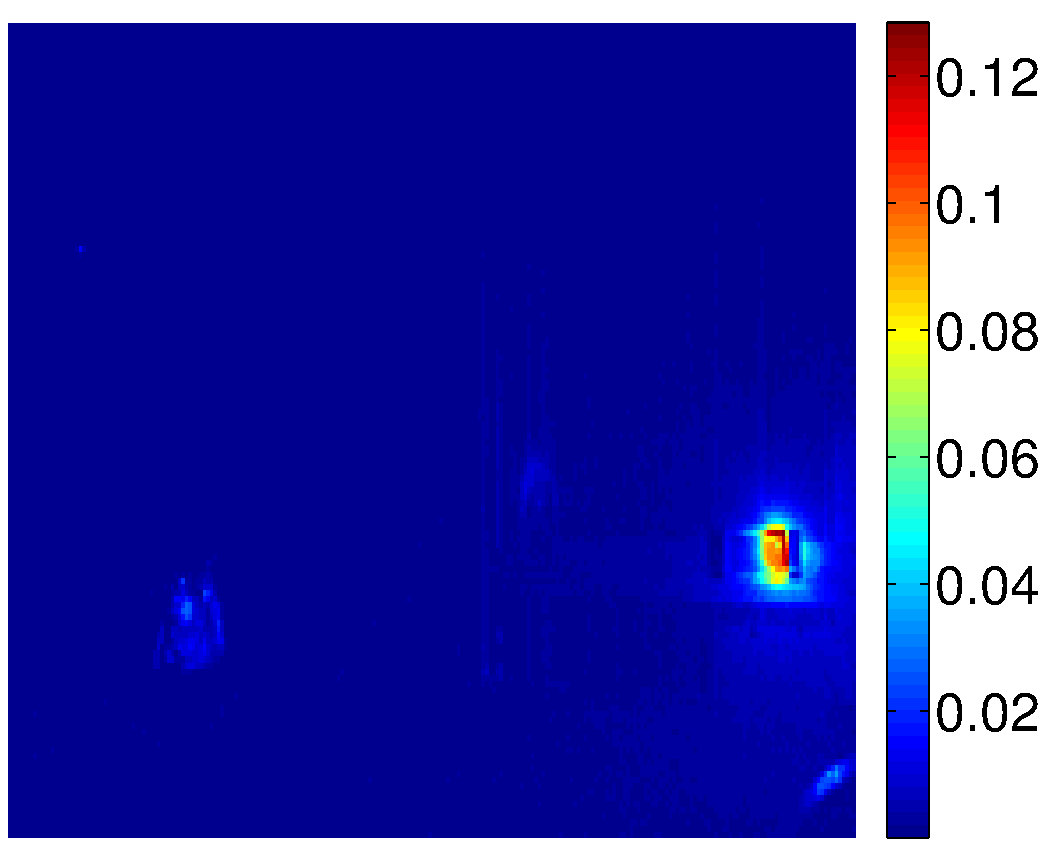
\includegraphics[width=0.45\textwidth]{chpt5_icca_vect/figs/flashing3_left1_orth.pdf}
    }
    \subfigure[\iccap]{
      \label{fig:chpt5:flashing3_1_opt}
      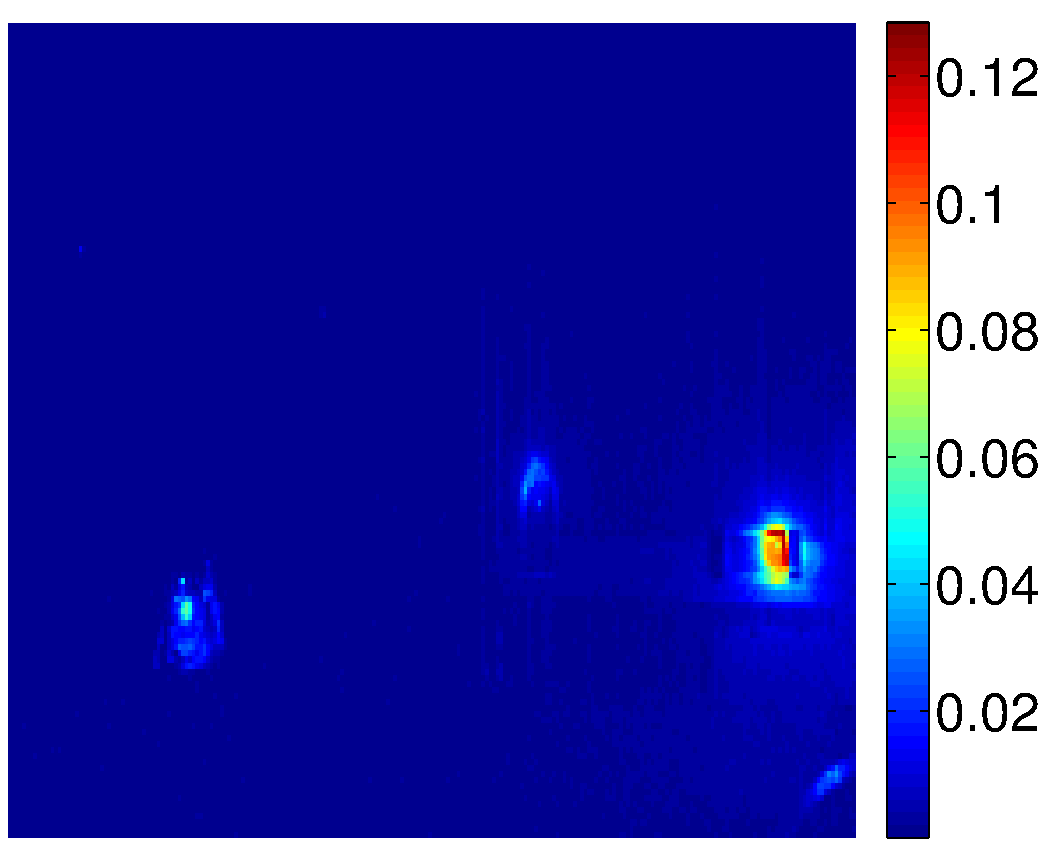
\includegraphics[width=0.45\textwidth]{chpt5_icca_vect/figs/flashing3_left1_opt.pdf}
    }
    \subfigure[CCA]{
      \label{fig:chpt5:flashing3_1_cca}
      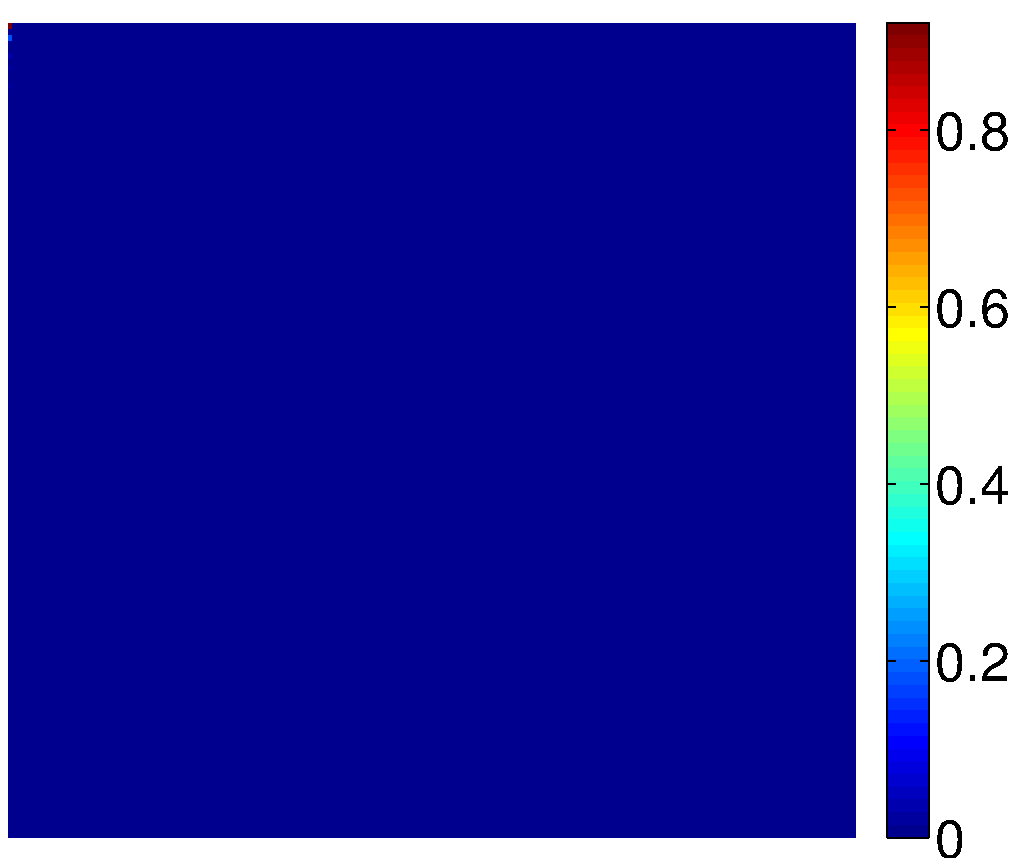
\includegraphics[width=0.45\textwidth]{chpt5_icca_vect/figs/flashing3_left1_cca.pdf}
    }
    \subfigure[ICCA minus \iccap]{
      \label{fig:chpt5:flashing3_1_diff1}
      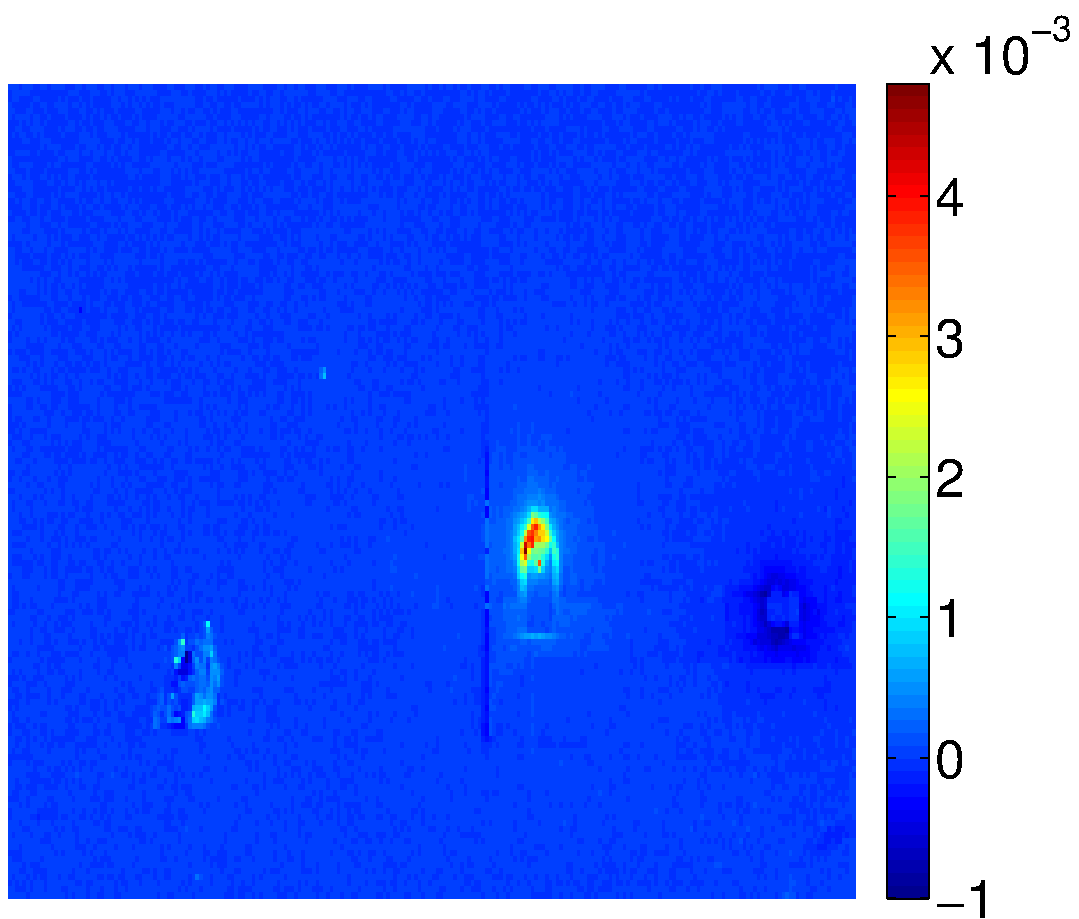
\includegraphics[width=0.45\textwidth]{chpt5_icca_vect/figs/flashing3_left1_diff_icca.pdf}
    }
    \subfigure[Orthogonal minus \iccap]{
      \label{fig:chpt5:flashing3_1_diff2}
      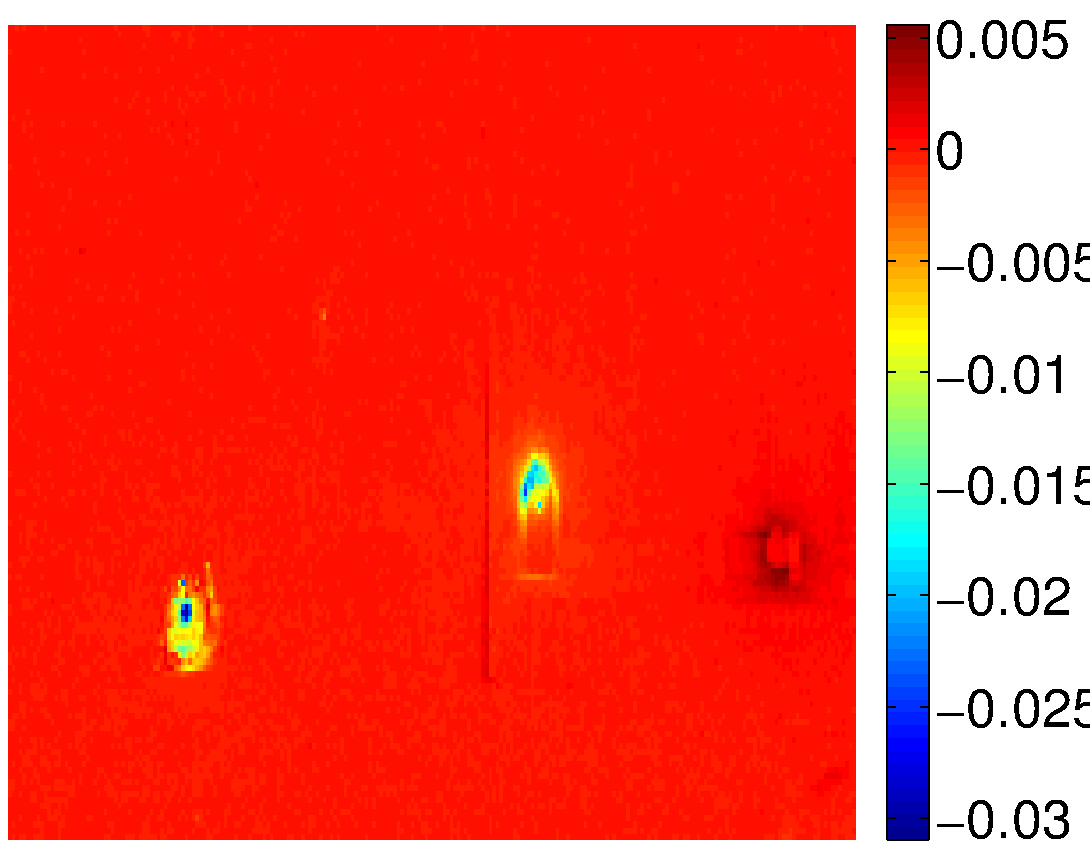
\includegraphics[width=0.45\textwidth]{chpt5_icca_vect/figs/flashing3_left1_diff_orth.pdf}
    }
    \caption{First canonical vector estimates for the left camera at frame 30. This corresponds
      to a total capture time of 1 second. (a)-(d) show the absolute value of the
      vectors displayed in an image so that large values indicate correlated
      pixels. (e)-(f) plot the difference between the ICCA estimate and the \iccap
      estimate and the orthogonal estimate and the \iccap estimate. Positive values
      indicate pixels that the \iccap estimate thinks are less correlated while negative
      values indicate pixels that the \iccap estimate thinks are more correlated. }
    \label{fig:chpt5:flashing3_1}
  \end{center}
\end{figure}

\begin{figure}
  \begin{center}
    \subfigure[ICCA]{
      \label{fig:chpt5:flashing1_1_plugin}
      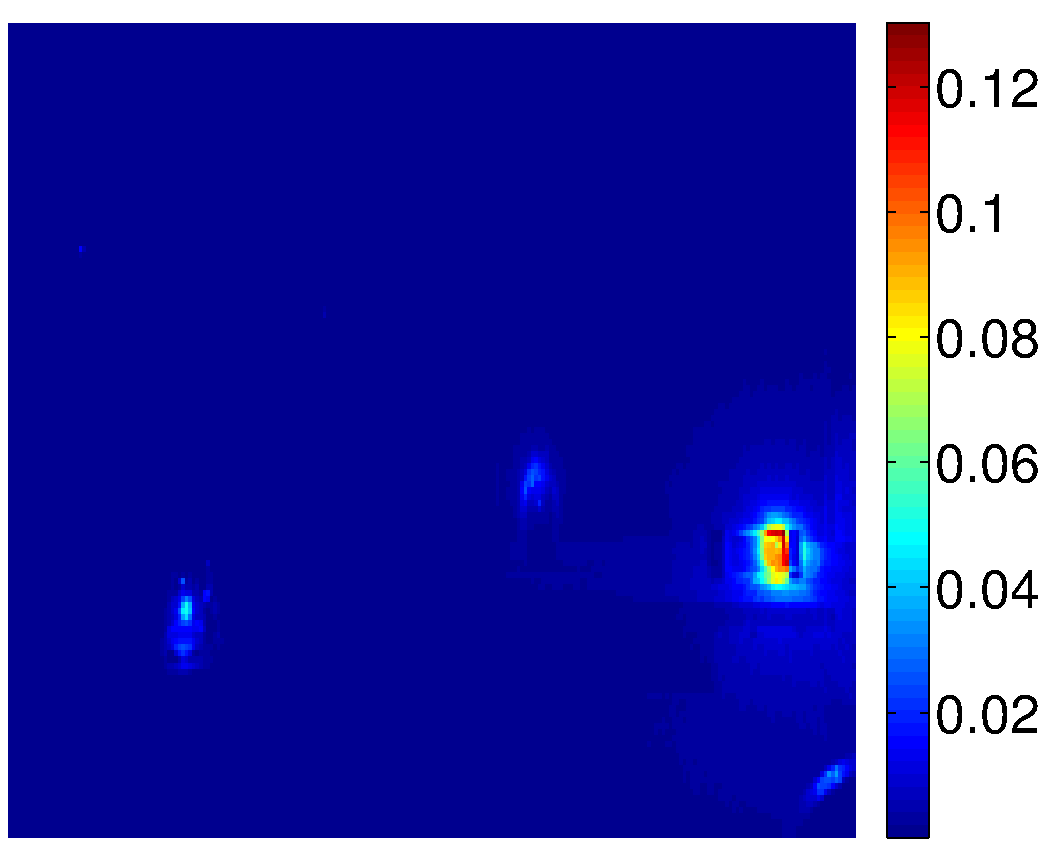
\includegraphics[width=0.45\textwidth]{chpt5_icca_vect/figs/flashing1_left1_icca.pdf}
    }
    \subfigure[Orthogonal]{
      \label{fig:chpt5:flashing1_1_orth}
      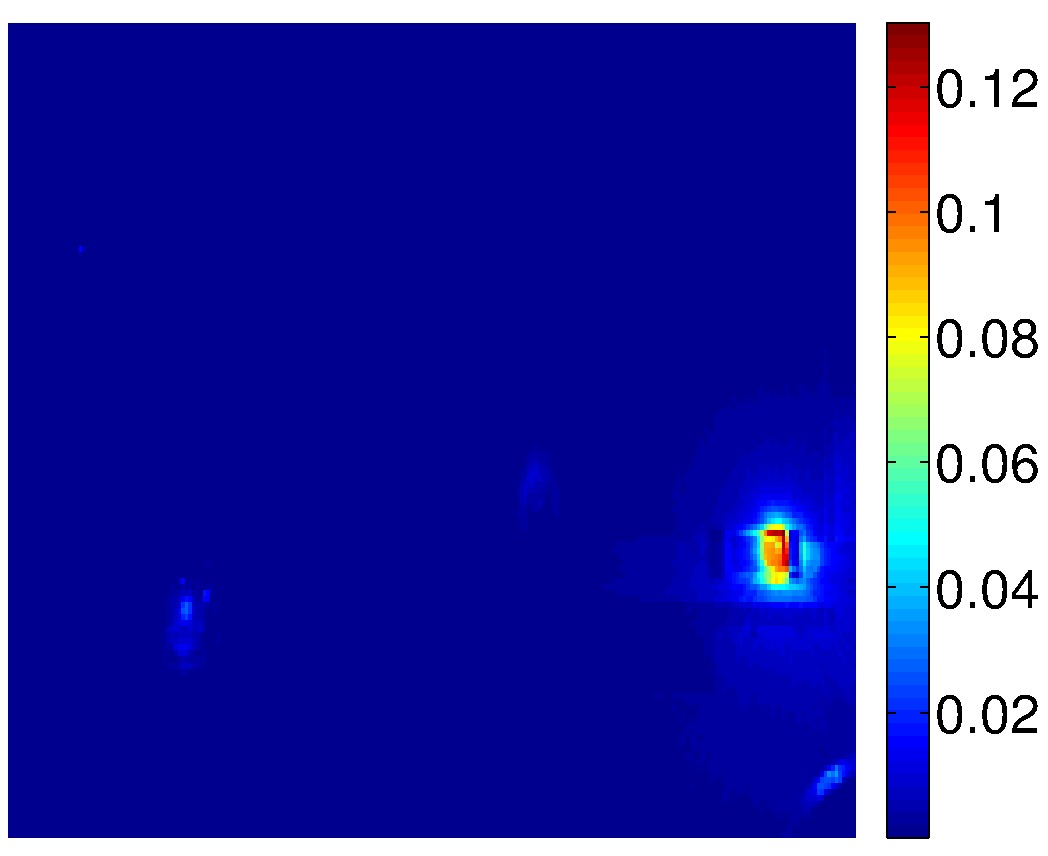
\includegraphics[width=0.45\textwidth]{chpt5_icca_vect/figs/flashing1_left1_orth.pdf}
    }
    \subfigure[\iccap]{
      \label{fig:chpt5:flashing1_1_opt}
      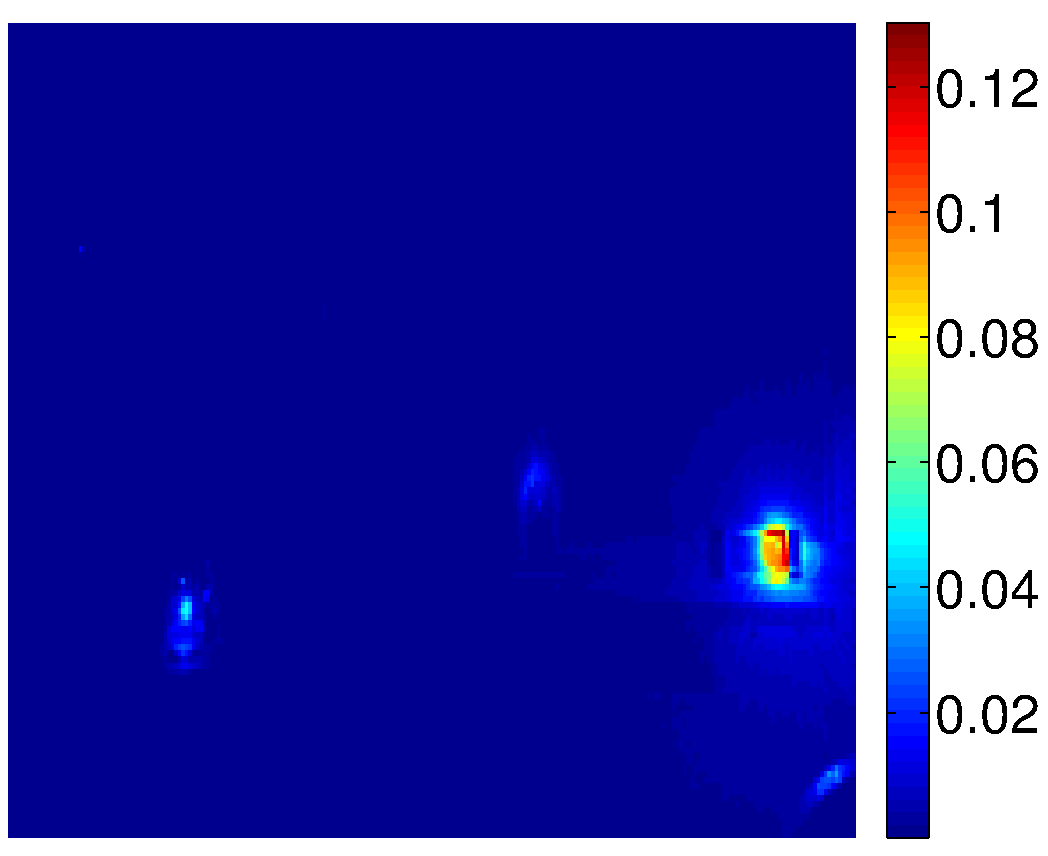
\includegraphics[width=0.45\textwidth]{chpt5_icca_vect/figs/flashing1_left1_opt.pdf}
    }
    \subfigure[CCA]{
      \label{fig:chpt5:flashing1_1_cca}
      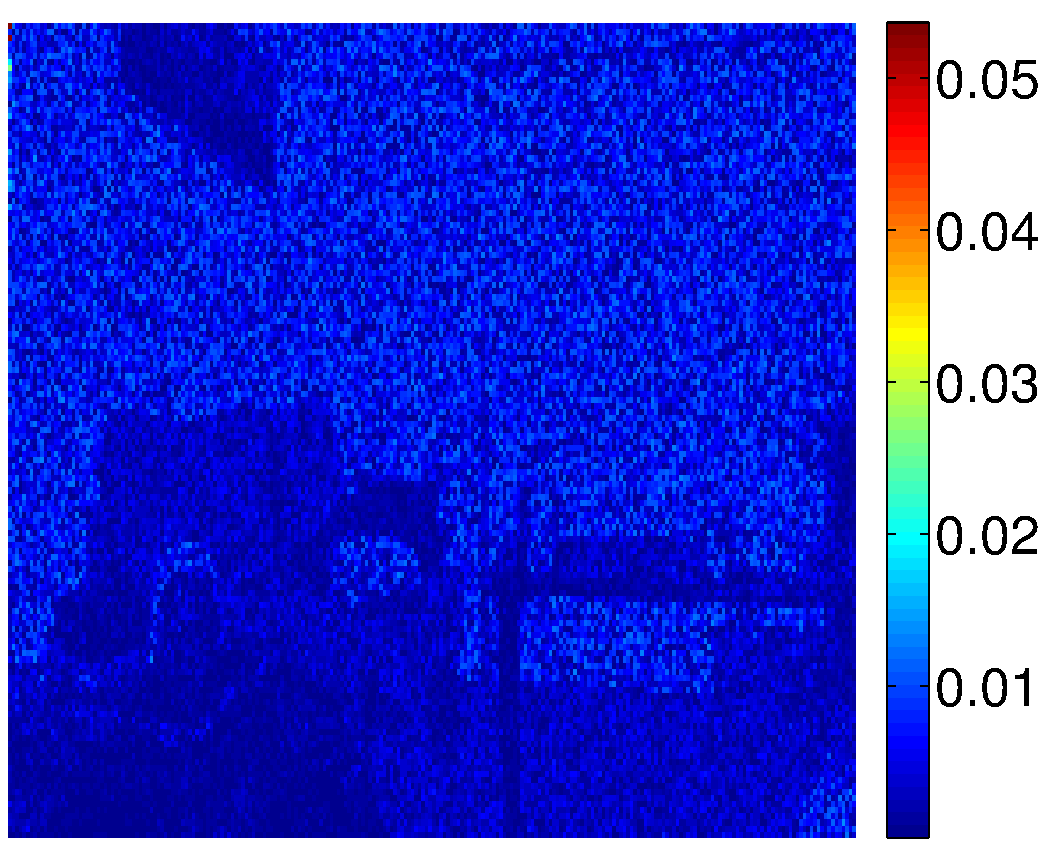
\includegraphics[width=0.45\textwidth]{chpt5_icca_vect/figs/flashing1_left1_cca.pdf}
    }
    \subfigure[ICCA minus \iccap]{
      \label{fig:chpt5:flashing1_1_diff1}
      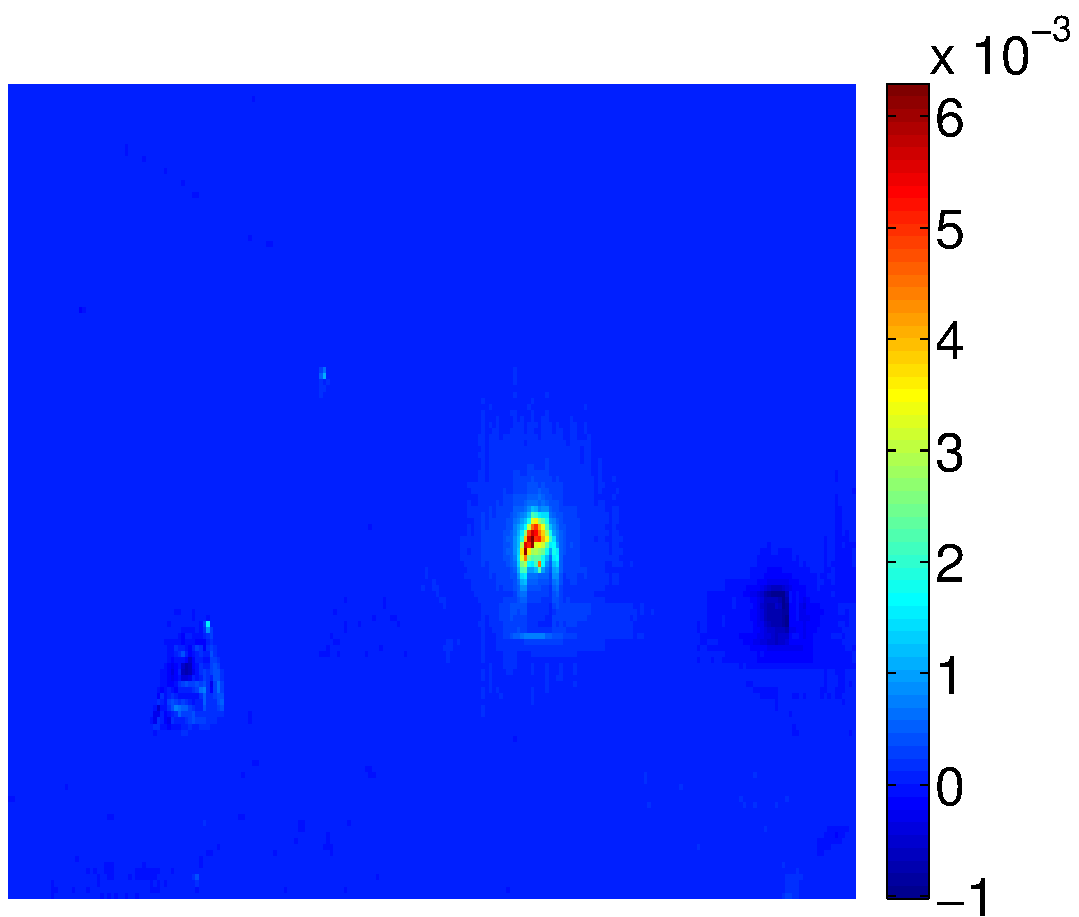
\includegraphics[width=0.45\textwidth]{chpt5_icca_vect/figs/flashing1_left1_diff_icca.pdf}
    }
    \subfigure[Orthogonal minus \iccap]{
      \label{fig:chpt5:flashing1_1_diff2}
      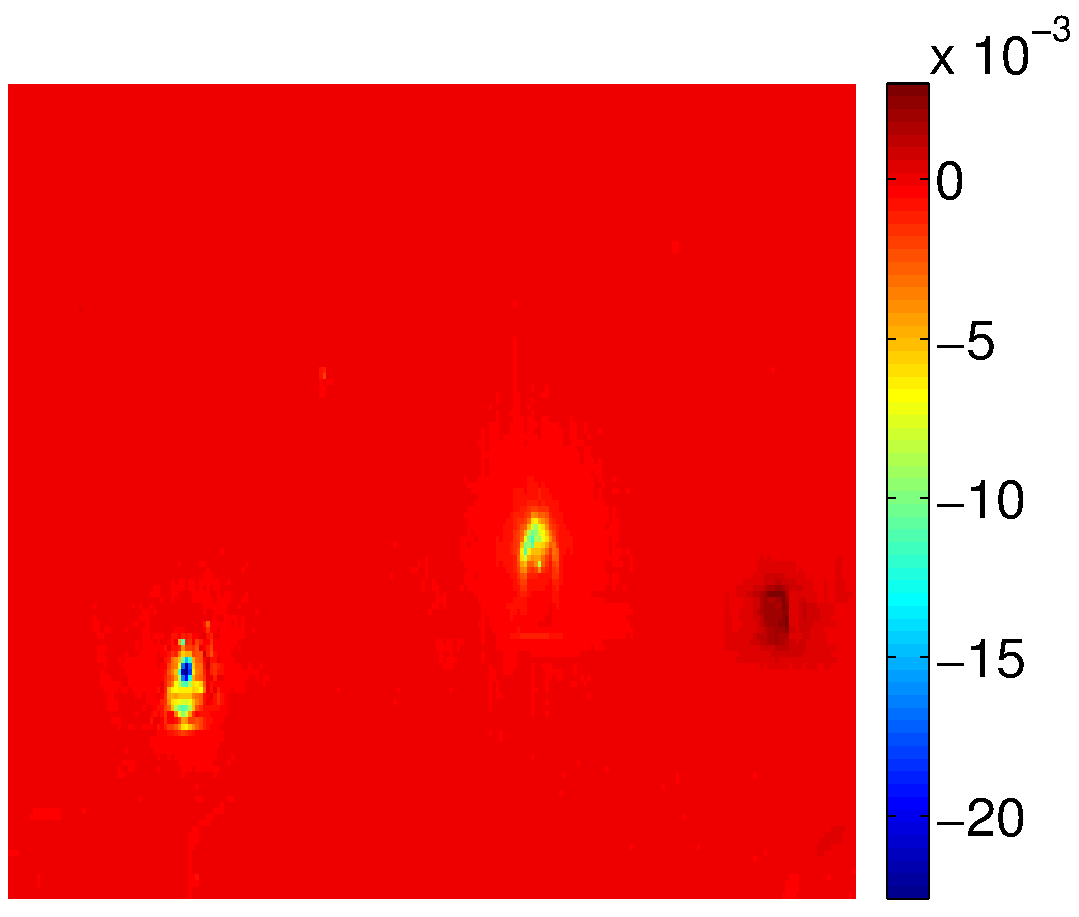
\includegraphics[width=0.45\textwidth]{chpt5_icca_vect/figs/flashing1_left1_diff_orth.pdf}
    }
    \caption{First canonical vector estimates for the left camera at frame 600. This corresponds
      to a total capture time of 20 seconds. (a)-(d) show the absolute value of the
      vectors displayed in an image so that large values indicate correlated
      pixels. (e)-(f) plot the difference between the ICCA estimate and the \iccap
      estimate and the orthogonal estimate and the \iccap estimate. Positive values
      indicate pixels that the \iccap estimate thinks are less correlated while negative
      values indicate pixels that the \iccap estimate thinks are more correlated. }
    \label{fig:chpt5:flashing1_1}
  \end{center}
\end{figure}

Figures \ref{fig:chpt5:flashing2_2} - \ref{fig:chpt5:flashing1_2} plot the second
canonical vector estimates for the left camera after frame 5, 30, and 600,
respectively. Each figure again plots the absolute value of the ICCA, orthogonal, \iccaps,
and empirical CCA canonical vector estimates. Each figure also plots the difference
between the ICCA and \iccap canonical vectors and the orthogonal and \iccap canonical
vectors. In these figures, pixels with negative values represent pixels that the \iccap
estimate believes are more correlated while positive values represent pixels that the
\iccap estimate believes are less correlated.

Similar to the estimates of the first canonical vector, we see that the empirical CCA
canonical vector estimate is just simply noise. The ICCA, orthogonal, and \iccap
estimates are all very similar and all identify source BPL, which is correlated to source
RPL in the right camera. Again, these estimates improve as we get more samples
(frames). Examining the difference plots in (e) and (f), we once again see that the ICCA
estimate is suboptimal as it places more weight on the independent source PH1 than the
\iccap estimate. The difference between the orthogonal and \iccap estimates is fairly
interesting. The orthogonal estimate places more weight on source PH2, while the \iccap
estimate places more weight on source PH1. Both of these sources are not correlated with
the police lights and so we conclude that the orthogonal and \iccap estimates do equally
well estimating the second canonical vector.

\begin{figure}
  \begin{center}
    \subfigure[ICCA]{
      \label{fig:chpt5:flashing2_2_plugin}
      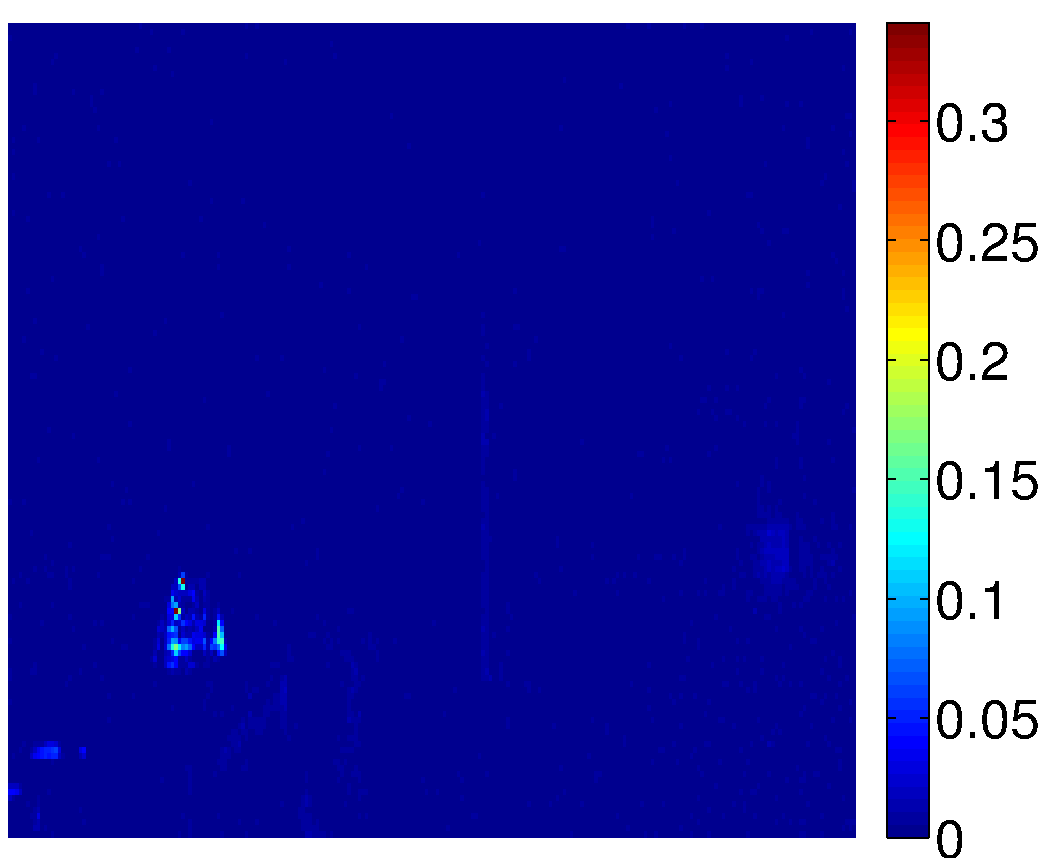
\includegraphics[width=0.45\textwidth]{chpt5_icca_vect/figs/flashing2_left2_icca.pdf}
    }
    \subfigure[Orthogonal]{
      \label{fig:chpt5:flashing2_2_orth}
      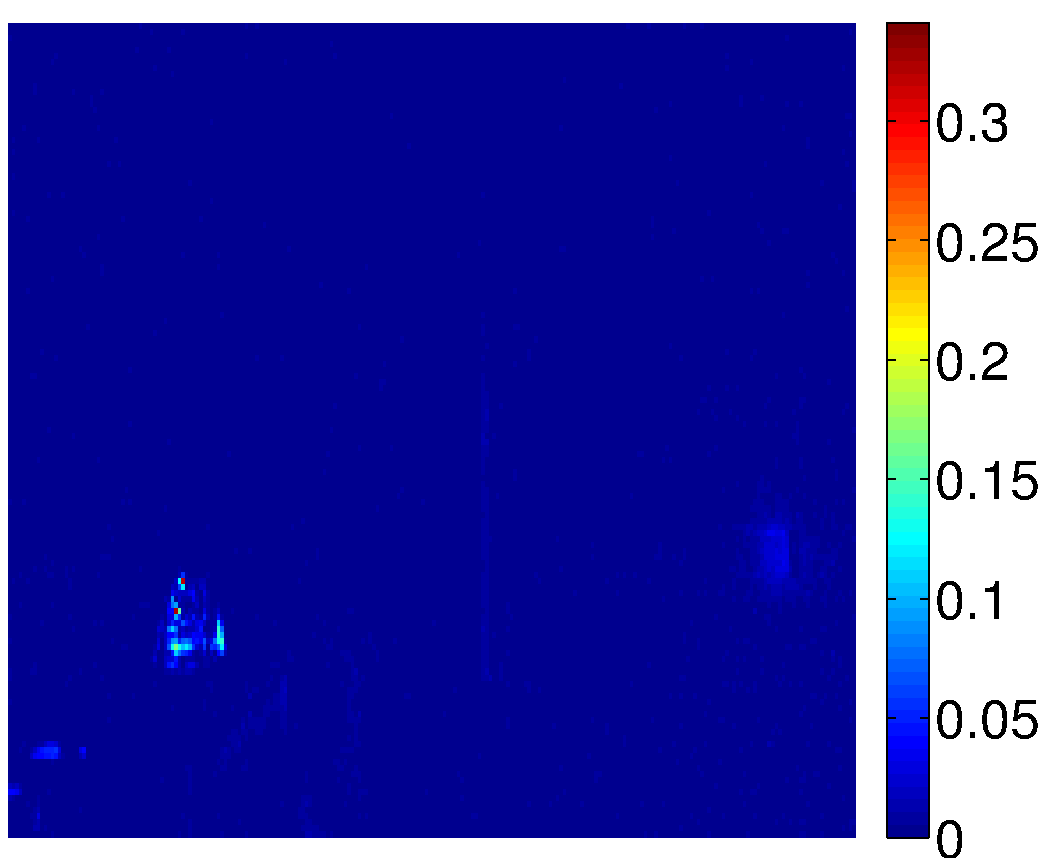
\includegraphics[width=0.45\textwidth]{chpt5_icca_vect/figs/flashing2_left2_orth.pdf}
    }
    \subfigure[\iccap]{
      \label{fig:chpt5:flashing2_2_opt}
      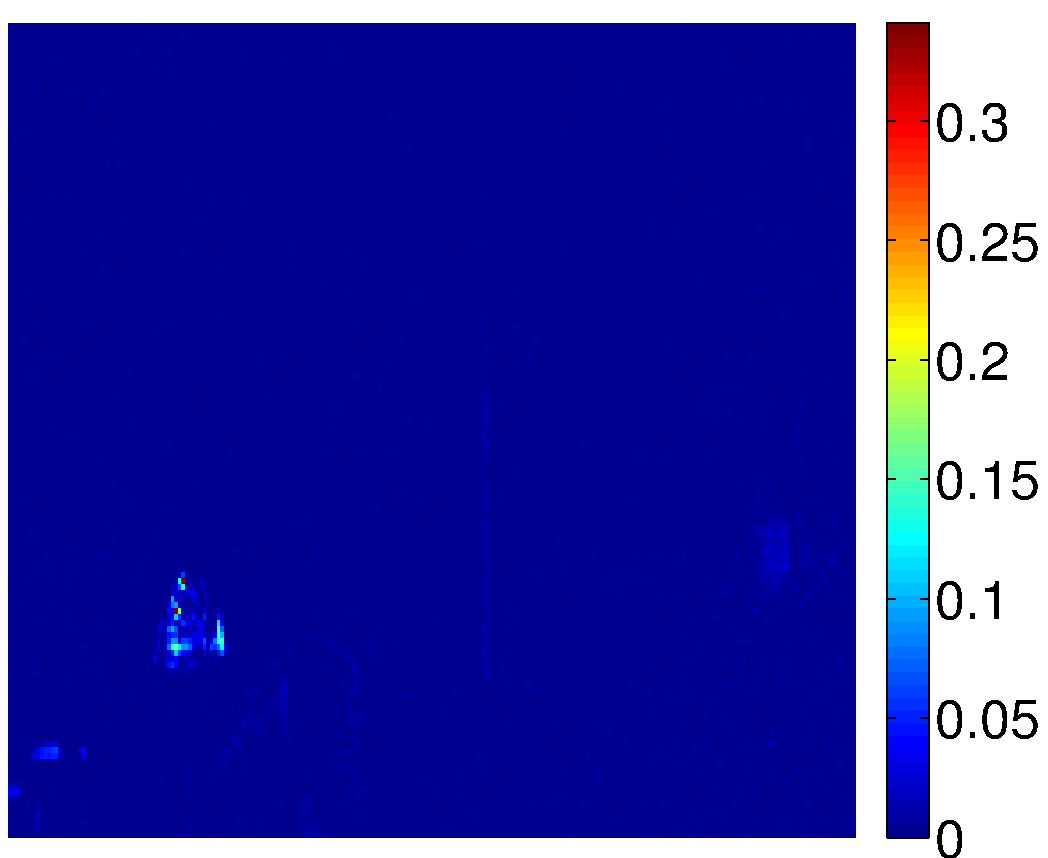
\includegraphics[width=0.45\textwidth]{chpt5_icca_vect/figs/flashing2_left2_opt.pdf}
    }
    \subfigure[CCA]{
      \label{fig:chpt5:flashing2_2_cca}
      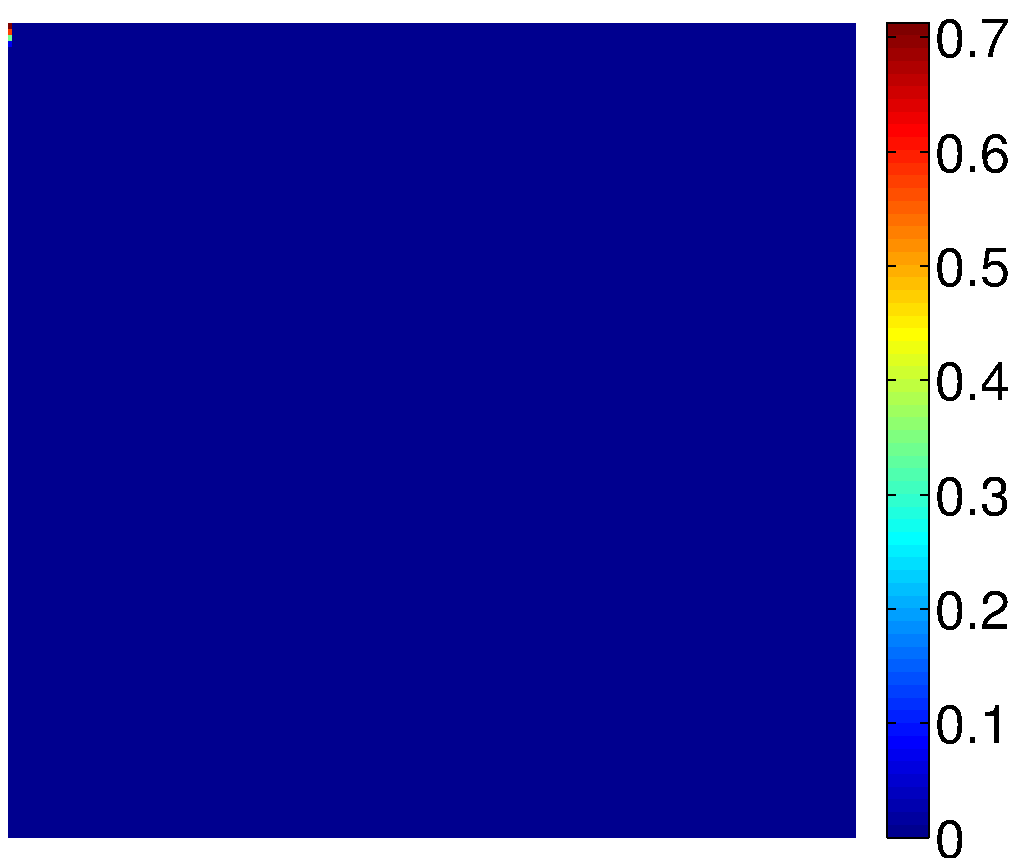
\includegraphics[width=0.45\textwidth]{chpt5_icca_vect/figs/flashing2_left2_cca.pdf}
    }
    \subfigure[ICCA minus \iccap]{
      \label{fig:chpt5:flashing2_2_diff1}
      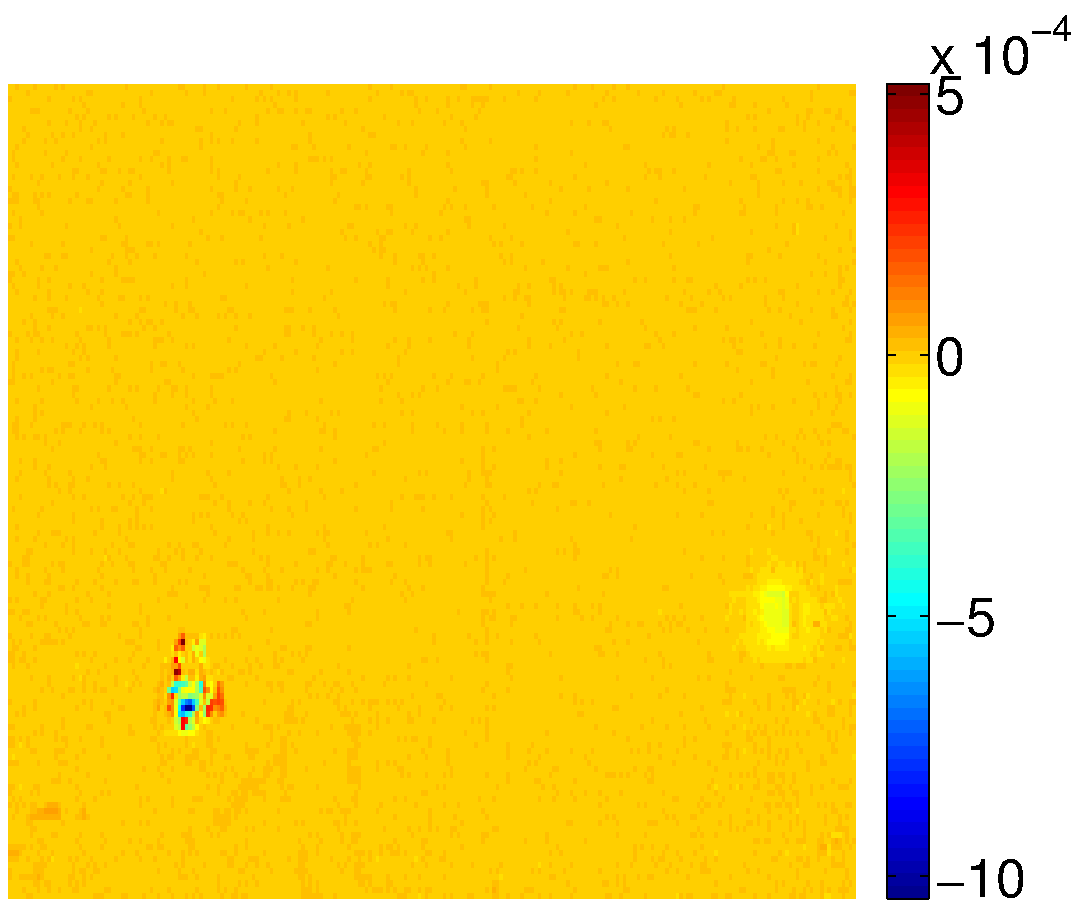
\includegraphics[width=0.45\textwidth]{chpt5_icca_vect/figs/flashing2_left2_diff_icca.pdf}
    }
    \subfigure[Orthogonal minus \iccap]{
      \label{fig:chpt5:flashing2_2_diff2}
      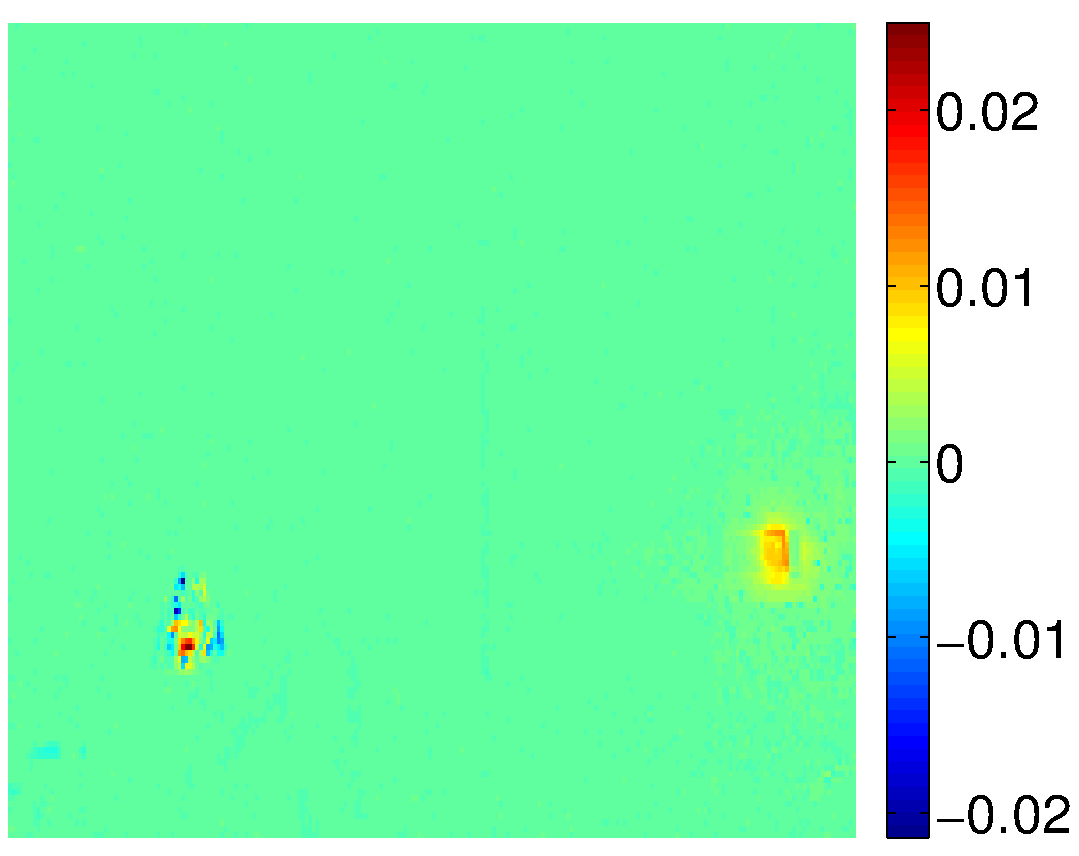
\includegraphics[width=0.45\textwidth]{chpt5_icca_vect/figs/flashing2_left2_diff_orth.pdf}
    }
    \caption{Second canonical vector estimates for the left camera at frame 5. This corresponds
      to a total capture time of 1/6 of a second. (a)-(d) show the absolute value of the
      vectors displayed in an image so that large values indicate correlated
      pixels. (e)-(f) plot the difference between the ICCA estimate and the \iccap
      estimate and the orthogonal estimate and the \iccap estimate. Positive values
      indicate pixels that the \iccap estimate thinks are less correlated while negative
      values indicate pixels that the \iccap estimate thinks are more correlated. }
    \label{fig:chpt5:flashing2_2}
  \end{center}
\end{figure}

\begin{figure}
  \begin{center}
    \subfigure[ICCA]{
      \label{fig:chpt5:flashing3_2_plugin}
      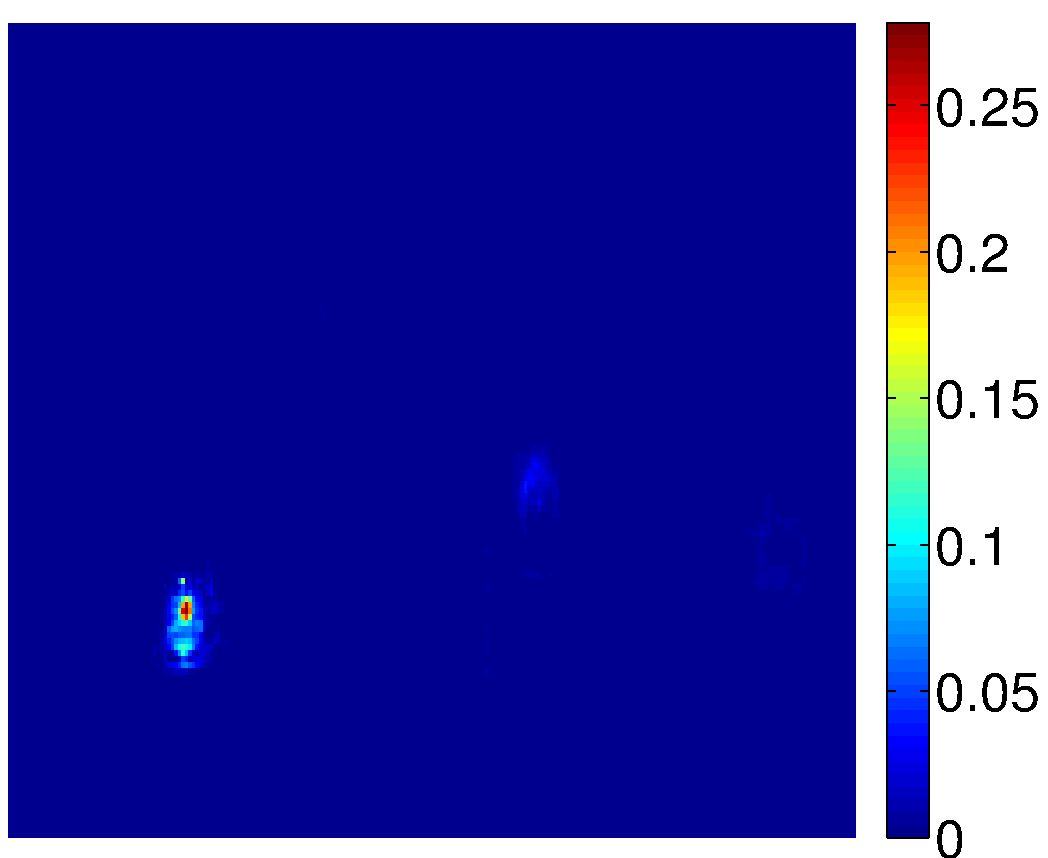
\includegraphics[width=0.45\textwidth]{chpt5_icca_vect/figs/flashing3_left2_icca.pdf}
    }
    \subfigure[Orthogonal]{
      \label{fig:chpt5:flashing3_2_orth}
      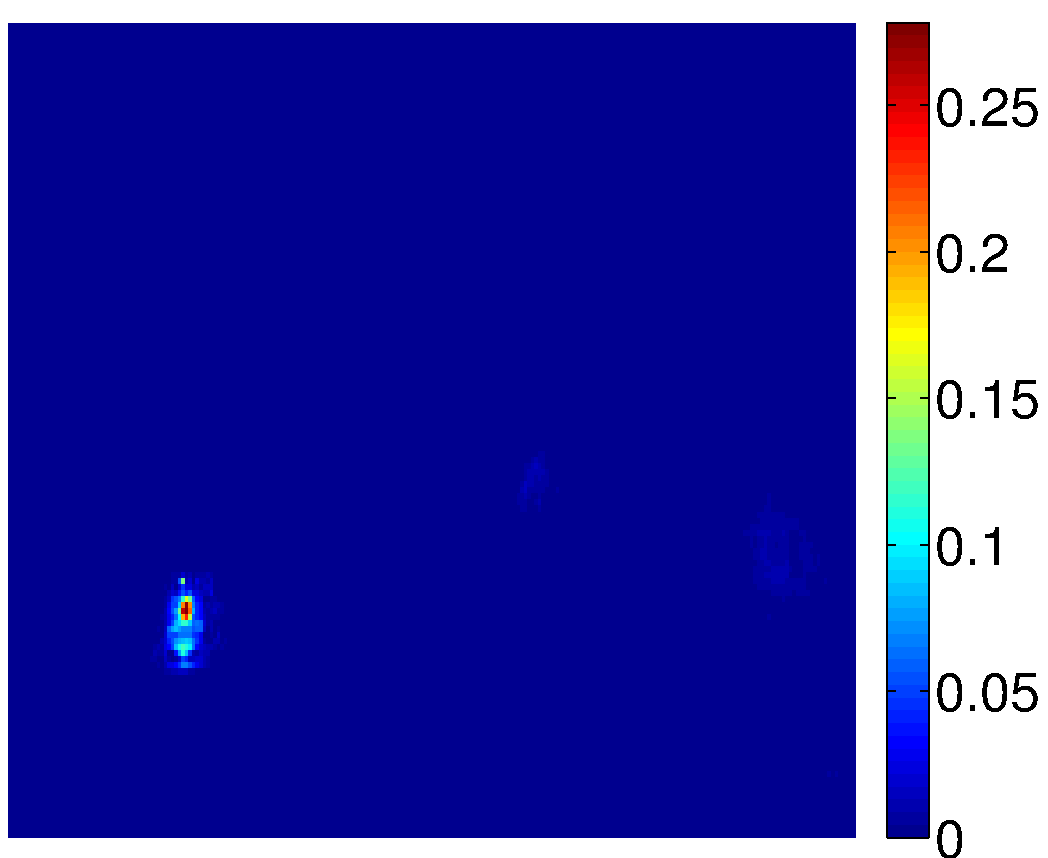
\includegraphics[width=0.45\textwidth]{chpt5_icca_vect/figs/flashing3_left2_orth.pdf}
    }
    \subfigure[\iccap]{
      \label{fig:chpt5:flashing3_2_opt}
      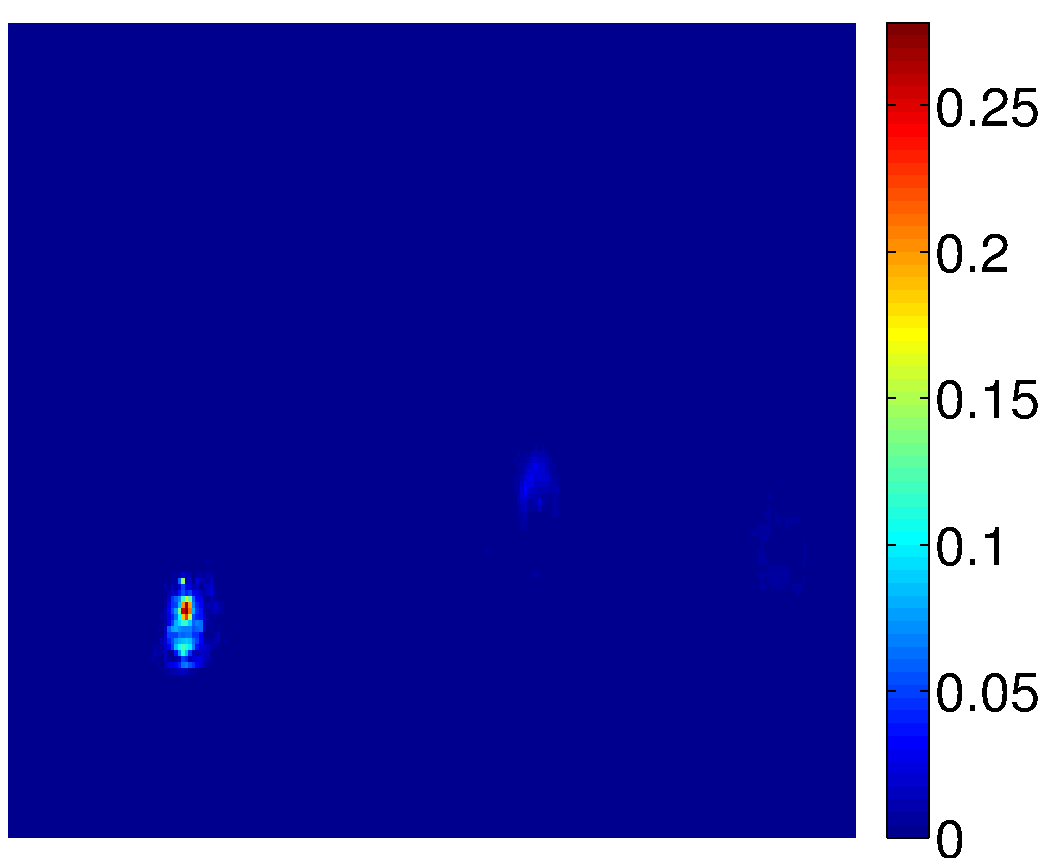
\includegraphics[width=0.45\textwidth]{chpt5_icca_vect/figs/flashing3_left2_opt.pdf}
    }
    \subfigure[CCA]{
      \label{fig:chpt5:flashing3_2_cca}
      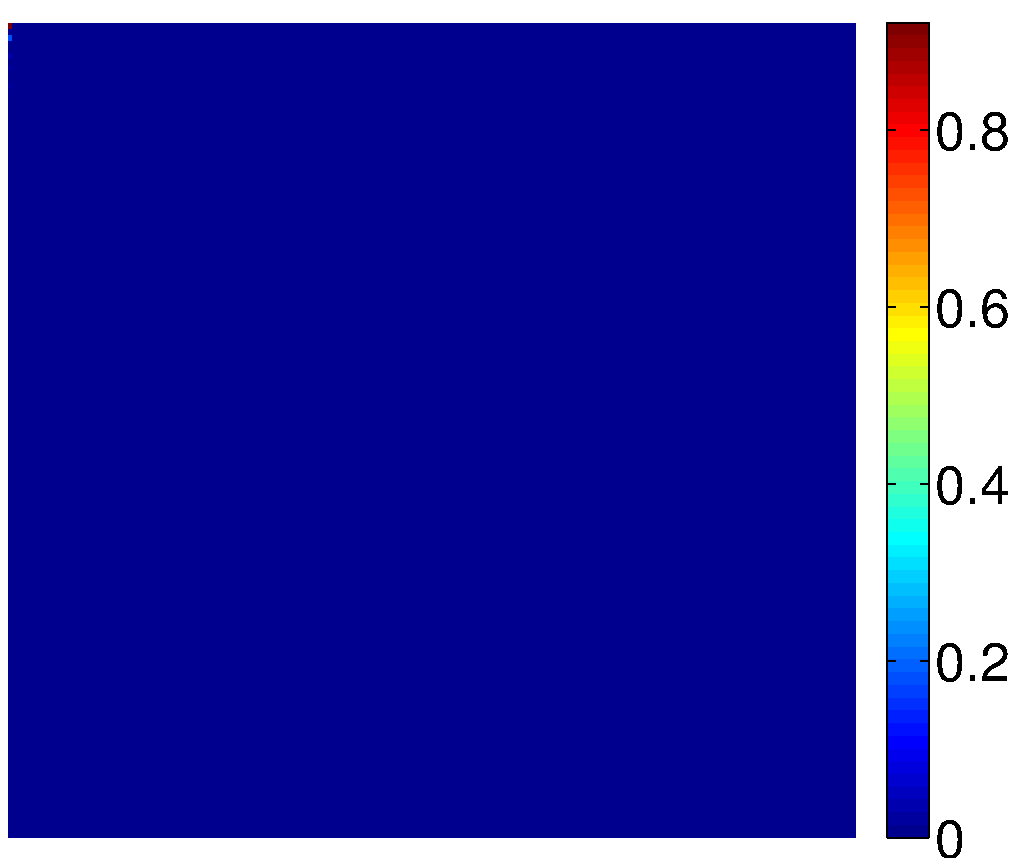
\includegraphics[width=0.45\textwidth]{chpt5_icca_vect/figs/flashing3_left2_cca.pdf}
    }
    \subfigure[ICCA minus \iccap]{
      \label{fig:chpt5:flashing3_2_diff1}
      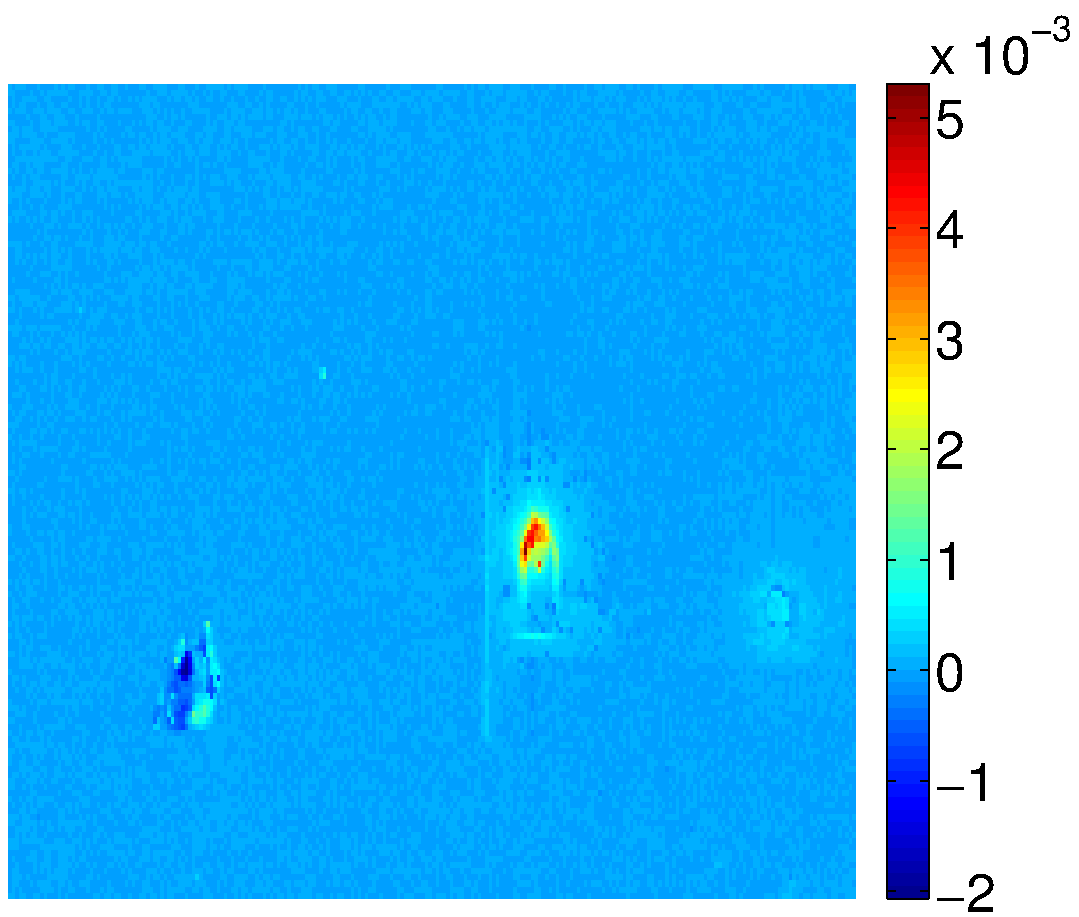
\includegraphics[width=0.45\textwidth]{chpt5_icca_vect/figs/flashing3_left2_diff_icca.pdf}
    }
    \subfigure[Orthogonal minus \iccap]{
      \label{fig:chpt5:flashing3_2_diff2}
      \includegraphics[width=0.45\textwidth]{chpt5_icca_vect/figs/flashing3_left2_diff_orth.pdf}
    }
    \caption{Second canonical vector estimates for the left camera at frame 30. This corresponds
      to a total capture time of 1 second. (a)-(d) show the absolute value of the
      vectors displayed in an image so that large values indicate correlated
      pixels. (e)-(f) plot the difference between the ICCA estimate and the \iccap
      estimate and the orthogonal estimate and the \iccap estimate. Positive values
      indicate pixels that the \iccap estimate thinks are less correlated while negative
      values indicate pixels that the \iccap estimate thinks are more correlated. }
    \label{fig:chpt5:flashing3_2}
  \end{center}
\end{figure}

\begin{figure}
  \begin{center}
    \subfigure[ICCA]{
      \label{fig:chpt5:flashing1_2_plugin}
      \includegraphics[width=0.45\textwidth]{chpt5_icca_vect/figs/flashing1_left2_icca.pdf}
    }
    \subfigure[Orthogonal]{
      \label{fig:chpt5:flashing1_2_orth}
      \includegraphics[width=0.45\textwidth]{chpt5_icca_vect/figs/flashing1_left2_orth.pdf}
    }
    \subfigure[\iccap]{
      \label{fig:chpt5:flashing1_2_opt}
      \includegraphics[width=0.45\textwidth]{chpt5_icca_vect/figs/flashing1_left2_opt.pdf}
    }
    \subfigure[CCA]{
      \label{fig:chpt5:flashing1_2_cca}
      \includegraphics[width=0.45\textwidth]{chpt5_icca_vect/figs/flashing1_left2_cca.pdf}
    }
    \subfigure[ICCA minus \iccap]{
      \label{fig:chpt5:flashing1_2_diff1}
      \includegraphics[width=0.45\textwidth]{chpt5_icca_vect/figs/flashing1_left2_diff_icca.pdf}
    }
    \subfigure[Orthogonal minus \iccap]{
      \label{fig:chpt5:flashing1_2_diff2}
      \includegraphics[width=0.45\textwidth]{chpt5_icca_vect/figs/flashing1_left2_diff_orth.pdf}
    }
    \caption{Second canonical vector estimates for the left camera at frame 600. This corresponds
      to a total capture time of 20 seconds. (a)-(d) show the absolute value of the
      vectors displayed in an image so that large values indicate correlated
      pixels. (e)-(f) plot the difference between the ICCA estimate and the \iccap
      estimate and the orthogonal estimate and the \iccap estimate. Positive values
      indicate pixels that the \iccap estimate thinks are less correlated while negative
      values indicate pixels that the \iccap estimate thinks are more correlated. }
    \label{fig:chpt5:flashing1_2}
  \end{center}
\end{figure}


\subsection{Audio-Audio Experiment}

We also explore the accuracy of the canonical vectors estimates on the audio-audio
experiment created in Chapter \ref{sec:chpt_cca_det}. In this experiment, we generate two
30 second audio sequences. Each sequence contains two pure-tones, which are amplitude
modulated (AM) at different frequencies. In addition we add uncorrelated coffee shop
noise, which is independent between each audio sequence. One pure-tone in each sequence is
amplitude modulated at a shared rate, inducing correlation between the audio
sequences. The remaining pure-tones are amplitude modulated at different rates, making
them independent of the shared AM tones. Our waveforms are
\be\ba
&a_1(t) = \frac{1}{3}s_1(t) + \frac{1}{3}s_2(t) + \frac{1}{3}n_1(t)\\
&a_2(t) = \frac{1}{3}s_3(t) + \frac{1}{3}s_4(t) + \frac{1}{3}n_2(t)
\ea\ee
where 
\be\ba
& s_1(t) = \frac{(1+\sin(2\pi t))}{2}\sin\left(2\pi\left(250t\right)\right)\\
& s_2(t) = \frac{(1+\cos(2\pi (3t))}{2}\sin\left(2\pi\left(400t\right)\right)\\
& s_3(t) = \frac{(1+\sin(2\pi t))}{2}\sin\left(2\pi\left(300t\right)\right)\\
& s_4(t) = \frac{(1+\cos(2\pi (5t))}{2}\sin\left(2\pi\left(550t\right)\right)\\
& n_1(t) = \text{independent coffee shop noise}. \\
& n_2(t) = \text{independent coffee shop noise}. \\
\ea\ee
All time sequences are generated with a sample rate of 44.1 kHz. Figure
\ref{fig:chpt5:aa_spectrograms} plots the spectrogram of each sequence and zooms in on a smaller
portion of the spectrum to see the AM sequences. Table \ref{tab:chpt5:aa_descrp}
summarizes each of our signals in each audio sequences.
\begin{table*}[ht!]
\centering
\begin{tabular}{c|c|c}\toprule
View & Source & Frequency\\
\midrule
$a_1(t)$ & 250 Hz pure tone & 1 Hz\\
& 400 Hz pure tone & 3 Hz\\
& coffee shop noise 1&\\
\midrule
$a_2(t)$ & 300 Hz pure tone & 1 Hz\\
& 550 Hz pure tone & 5 Hz\\
& coffee shop noise 2&\\
\bottomrule
\end{tabular}
\caption{Summary of the audio sources. The 250 Hz pure tone in Audio 1 is amplitude
  modulated at the same frequency as the 300 Hz pure tone in Audio 2 and is thus
  correlated with it.}
\label{tab:chpt5:aa_descrp}
\end{table*}

To post-process the data, we separate the audio streams into equal window sizes of 2940
time points, corresponding to a time interval of 1/15 second. On each window, we run a
4096 point FFT and take the magnitude of the first 2049 points as a feature vector. We
then stack the feature vectors for all windows into a matrix and subtract the mean,
resulting in $2049 \times 450$ matrices $X_{a_1}$ and $Y_{a_2}$.


\begin{figure}
  \begin{center}
    \subfigure[Full Spectrogram of $a_1(t)$]{
      \label{fig:chpt4:aa1_full_spec}
      \includegraphics[width=0.47\textwidth]{chpt5_icca_vect/figs/aa1_full_spect.pdf}
    }
    \subfigure[Zoomed Spectrogram of $a_1(t)$]{
      \label{fig:chpt4:aa1_spec_zoom}
      \includegraphics[width=0.47\textwidth]{chpt5_icca_vect/figs/aa1_zoom_spect.pdf}
    }   
    \subfigure[Full Spectrogram of $a_2(t)$]{
      \label{fig:chpt4:aa2_full_spec}
      \includegraphics[width=0.47\textwidth]{chpt5_icca_vect/figs/aa2_full_spect.pdf}
    }
    \subfigure[Zoomed Spectrogram of $a_2(t)$]{
      \label{fig:chpt4:aa2_spec_zoom}
      \includegraphics[width=0.47\textwidth]{chpt5_icca_vect/figs/aa2_zoom_spect.pdf}
    }   
    \caption{(a) Full spectrogram of $a_1(t)$. (b) Zoomed in spectrogram of $a_1(t)$ to
      see the 2 sources at 250 Hz and 400 Hz. (c) Full spectrogram of $a_2(t)$ (d) Zoomed
      in spectrogram of $a_2(t)$ to see the 2 sources at 300 Hz and 550 Hz. The 250 Hz
      signal in $a_1(t)$ is amplitude modulated at the same frequency as the 300 Hz signal
      in $a_2(t)$.}
    \label{fig:chpt5:aa_spectrograms}
  \end{center}
\end{figure}

Figures \ref{fig:chpt5:aa1} and \ref{fig:chpt5:aa2} plot the first canonical vector
estimates for the first and second audio steams, respectively. Each figure plots the
absolute value of the canonical vectors, whose entries correspond to frequencies. Thus,
large weights correspond to frequencies that are correlated between the two audio
streams. Each figures plots the canonical vector estimates for 3 different frames,
corresponding to 1/6 of a second, 1 second, and 20 seconds.

From these figures, we once again see that the empirical CCA estimates are very inaccurate
in the low-sample regime, lending credence to Conjecture \ref{conj:icca_vect}. We also
observe that the ICCA, orthogonal, and \iccap estimates are all very similar for this
experiment. Each identifies the correlated AM signal at 250 HZ (Figure
\ref{fig:chpt5:aa1}) and 300 Hz (Figure \ref{fig:chpt5:aa2}). In each figure, we plot a
zoomed in version of canonical vector estimates at the independent AM frequencies of 400 Hz
(Figure \ref{fig:chpt5:aa1_3_zoom}) and 550 Hz (Figure \ref{fig:chpt5:aa2_3_zoom}). In
both figures we observe a slight difference in the orthogonal estimate. In both
cases, it places a larger weight on this independent AM signal than the ICCA and
\iccap estimates. This is not desirable as this signal is not correlated across the audio
streams.

Therefore, in this application, the orthogonal estimate performs the worst while the
ICCA and \iccap estimates perform equally. This is due to the fact that the principle
components for the audio streams contain frequency components from both present signals
(see Figure \ref{fig:chpt4:aa_pca}). Therefore, $\Uktil$ is not identity, and we
empirically see the sub-optimality of the orthogonal estimate that we theoretically predicted.

\begin{figure}
  \begin{center}
    \subfigure[Frame 5]{
      \label{fig:chpt5:aa1_1}
      \includegraphics[width=0.45\textwidth]{chpt5_icca_vect/figs/aa1_1.pdf}
    }
    \subfigure[Frame 15]{
      \label{fig:chpt5:aa1_2}
      \includegraphics[width=0.45\textwidth]{chpt5_icca_vect/figs/aa1_2.pdf}
    }
    \subfigure[Frame 300]{
      \label{fig:chpt5:aa1_3}
      \includegraphics[width=0.45\textwidth]{chpt5_icca_vect/figs/aa1_3.pdf}
    }
    \subfigure[Frame 300 - Zoomed]{
      \label{fig:chpt5:aa1_3_zoom}
      \includegraphics[width=0.45\textwidth]{chpt5_icca_vect/figs/aa1_3_zoom.pdf}
    }
    \caption{Canonical vectors estimates for the first audio stream at 3 different
      frames. One frame corresponds to 1/15 seconds. Frequencies with large weights are
      those that the algorithms mark as correlated with frequencies with large weights in
      Figure \ref{fig:chpt5:aa2}.}
    \label{fig:chpt5:aa1}
  \end{center}
\end{figure}

\begin{figure}
  \begin{center}
    \subfigure[Frame 5]{
      \label{fig:chpt5:aa2_1}
      \includegraphics[width=0.45\textwidth]{chpt5_icca_vect/figs/aa2_1.pdf}
    }
    \subfigure[Frame 15]{
      \label{fig:chpt5:aa2_2}
      \includegraphics[width=0.45\textwidth]{chpt5_icca_vect/figs/aa2_2.pdf}
    }
    \subfigure[Frame 300]{
      \label{fig:chpt5:aa2_3}
      \includegraphics[width=0.45\textwidth]{chpt5_icca_vect/figs/aa2_3.pdf}
    }
    \subfigure[Frame 300 - Zoomed]{
      \label{fig:chpt5:aa2_3_zoom}
      \includegraphics[width=0.45\textwidth]{chpt5_icca_vect/figs/aa2_3_zoom.pdf}
    }
    \caption{Canonical vectors estimates for the second audio stream at 3 different
      frames. One frame corresponds to 1/15 seconds. Frequencies with large weights are
      those that the algorithms mark as correlated with frequencies with large weights in
      Figure \ref{fig:chpt5:aa1}.}
    \label{fig:chpt5:aa2}
  \end{center}
\end{figure}



\section{Proof of Theorem \ref{th:icca_opt}, Theorem \ref{th:vect_opt}, Corollary
  \ref{corr:icca_vects}, and Theorem \ref{th:icca_vect_miss}}\label{sec:chpt5:proofs1}

We will prove Theorem \ref{th:icca_opt} for $\lambda_x^{\text{opt}}$ and by a similar
argument assume the result for $\lambda_y^{\text{opt}}$. By the unitary invariance of the
Frobenius norm, we have
\be
\|W_x - \Uxhat\diag(\lambda_x)\Uktilhat\|_F = \|\Uxhat^HW_x\Uktilhat^H - \diag(\lambda_x)\|_F.
\ee
Substituting the definition of the population canonical vectors in
(\ref{eq:chpt5:pop_cca_vects}), we have
\be
\|\Uxhat^HW_x\Uktilhat^H - \diag(\lambda_x)\|_F =
\|\Uxhat^H\Ux\left(\Tx+I_{\kx}\right)^{-1/2}\Uktil\Uktilhat^H - \diag(\lambda_x)\|_F.
\ee
Let $A = \Uxhat^H\Ux\left(\Tx+I_{\kx}\right)^{-1/2}\Uktil\Uktilhat^H$. By assumption, we
have that $\Uktilhat$ is a consistent estimator of $\Uktil$ so that
$\Uktil\Uktilhat^H=I_{\kx}$. Therefore $A =
\Uxhat^H\Ux\left(\Tx+I_{\kx}\right)^{-1/2}$. Therefore, our optimization problem is
\be
\lambda_x^{\text{opt}} = \argmin_{\lambda_x}\|A-\diag(\lambda_x)\|_F.
\ee
By Lemma 4.1 and Corollary 4.1 from \cite{nadakuditi2014optshrink}, we have that 
\be
\lambda_x^{\text{opt}} = \diag(A),
\ee
which completes the proof of Theorem \ref{th:icca_opt}. 

We next turn toward Theorem \ref{th:vect_opt}. First, Theorem \ref{th:vect_opt} b) follows
immediately from Theorem 2.9 in 
\cite{benaych2012singular}. To prove part a), we note that by Theorem \ref{th:icca_opt}, we
have that
\be
\lambda_{x,\text{opt}}^{(i)} = A_{ii},
\ee
where $A$ is defined above. Examining the diagonal entries of this matrix, we have
\be
A_{ii} = \frac{\widehat{u}_x^{(i)H}u_x^{(i)}}{\sqrt{\left(\tx_i\right)^2 + 1}}.
\ee
To complete the proof, we must characterize the limiting behavior of these quantities. Let
\beq\label{eq:chpt5:sig_def}
\sigma_x^{(i)} = D_{\mu_{Z_x}}^{-1}\left(1/\left(\tx_1\right)^2\right).
\eeq
Theorem 2.10 a) of \cite{benaych2012singular} showed that
\be
\left|\langle \widehat{u}_x^{(i)}, u_{x}^{(i)}\rangle \right|^2\convas
\frac{-2\varphi_{\mu_{Z_x}}\left(\sigma_x^{(i)}\right)}{\left(\tx_i\right)^2D^\prime_{\mu_{Z_x}}\left(\sigma_x^{(i)}\right)},
\ee
where for any probability measure $\mu$,
\be
\varphi_{\mu}(z) = \int\frac{z}{z^2-t^2}d\mu(t).
\ee
We note that there is a ambiguity in the sign (or phase, when complex value) of these
singular vectors. While we use the consistency assumption to get
$\Uktil\Uktilhat^H=I_{\kx}$, we note that the sign of $\Uxhat$ is coupled with the sign of
$\Uktilhat$ and so we may take the positive square root of the above expression. Finally,
we know that by definition in (\ref{eq:chpt5:sig_def}),  
\be
1/\left(\tx_u\right)^2 = D_{\mu_{Z_x}}\left(\sigma_x^{(i)}\right).
\ee
Substituting these expressions into the diagonal elements of $A$, we arrive at our theorem
conclusion, 
\be\ba
&\lambda_{x,\text{opt}}^{(i)}&&\convas
\frac{\sqrt{\frac{-2D_{\mu_{Z_x}}\left(\sigma_x^{(i)}\right)\varphi_{\mu_{Z_x}}\left(\sigma_x^{(i)}\right)}{D^\prime_{\mu_{Z_x}}\left(\sigma_x^{(i)}\right)}}}{\sqrt{\frac{1}{D_{\mu_{Z_x}}\left(\sigma_x^{(i)}\right)}
    +1 }}\\
&&& = D_{\mu_{Z_x}}\left(\sigma_x^{(i)}\right)\sqrt{\frac{-2\varphi_{\mu_{Z_x}}\left(\sigma_x^{(i)}\right)}{D^\prime_{\mu_{Z_x}}\left(\sigma_x^{(i)}\right)\left(D_{\mu_{Z_x}}\left(\sigma_x^{(i)}\right)+1\right)}}
\ea\ee
A similar argument proves the result for $\lambda_{y,\text{opt}}^{(i)}$. 

Next, we prove Corollary \ref{corr:icca_vects} by providing the explicit forms of the $D$
transform and its derivative when we have Gaussian data as in (\ref{eq:chpt5:data_model}). From
\cite{paul2007asymptotics,asendorf2013performance}, we have that
\beq\label{eq:chpt5:svd_acc_vect}
\left|\langle \widehat{u}_x^{(i)}, u_{x}^{(i)}\rangle \right|^2\convas
\begin{cases}\frac{\left(\tx_i\right)^4-c_x}{\left(\tx_1\right)^4 + \left(\tx_i\right)^2c_x} &
  \text{ if } \tx_i > c_x^{1/4} \\ 0 & \text{o.w.} \end{cases},
\eeq
and
\beq\label{eq:chpt5:svd_acc_sv}
\left(\widehat{\theta}^{(x)}_i\right)^2\convas \begin{cases} \left(\tx_i\right)^2 +
  c_x+\frac{c_x}{\left(\tx_i\right)^2} & \text{ if } \tx_i > c_x^{1/4}\\ c_x + 2\sqrt{c_x}
  & \text{o.w.} \end{cases}.
\eeq
Substituting these expressions into $A_{ii}$ and the plug-in weights and
performing some minor algebra yields the result. A similar argument proves the result for
the $y$ weights.

Finally, we prove Theorem \ref{th:icca_vect_miss}. To prove this theorem, we follow the
same steps as the proof for Theorem 4.7.1 of Chapter 4. We omit the steps here to save space
as they are exactly the same. The main result of these proof steps
is that we replace $\Tx$ with $\gamma_x\Tx$ and $\Ty$ with $\gamma_y\Ty$. We additionally
notes that when we are below the phase transition, this analysis shows that
\be\ba
&X\to \gamma_x Z_x\\
&Y\to \gamma_y Z_y\\
\ea\ee
and so the estimates of $\tx_i$ and $\ty_i$ below the phase transition change by a factor
of $\gamma_x$ and $\gamma_y$, respectively. Making these substitutions in Corollary
\ref{corr:icca_vects} yields the expressions in Theorem \ref{th:icca_vect_miss}. 

\section{Proof of Theorem \ref{th:icca_acc}, Corollary \ref{corr:cca_vect_acc}, and Theorem \ref{th:orth_acc}}\label{sec:chpt5:proofs2}

We begin with our definition of accuracy in (\ref{eq:chpt5:cca_vect_acc})
\be
\text{ACC}^{(i)}(\lambda) =
\frac{\left(\Uktil^{(i)H}\left(\Tx +
      I_{\kx}\right)^{-1/2}\Ux^H\Uxcir\Lambda\Uktilhat^{(i)}\right)^2}{ \left(\Uktil^{(i)H}\left(\Tx
      + I_{\kx}\right)^{-1}\Uktil^{(i)}\right) \left(\Uktilhat^{(i)H}\Lambda^2\Uktilhat^{(i)}\right)}.
\ee
Using the assumption that $\Uktilhat$ is a consistent estimator of $\Uktil$, we have that
in the considered asymptotic regime, $\Uktilhat\to\Uktilhat$. Therefore, the numerator of
the above expression becomes 
\be
\left[\sum_{j=1}^{\kx}\frac{\left(\Uktil^{(i)}\right)_j^2\langle u_x^{(j)},
    \widehat{u}_x^{(j)}\rangle\lambda_j}{\sqrt{\left(\tx_j\right)^2+1}} + \sum_{j\neq\ell}^{\kx}
  \frac{\left(\Uktil^{(i)}\right)_j\left(\Uktil^{(i)}\right)_\ell \langle u_x^{(j)},
    \widehat{u}_x^{(\ell)} \rangle\lambda_\ell}{\sqrt{\left(\tx_j\right)^2+1}}\right]^2.
\ee
In \cite{benaych2012singular}, it was shown that for $j\neq\ell$ when $\left(\tx_i\right)^2
>1/D_{\mu_{Z_x}}(b_x)$ that $\langle u_x^{(j)}, \widehat{u}_x^{(\ell)} \rangle\convas
0$. Therefore, the numerator becomes
\be
\left[\sum_{j=1}^{\kx}\frac{\left(\Uktil^{(i)}\right)_j^2\langle u_x^{(j)},
    \widehat{u}_x^{(j)}\rangle\lambda_j}{\sqrt{\left(\tx_j\right)^2+1}}\right]^2.
\ee
In this regime, we have that from our Proof of Theorem \ref{th:icca_opt}
\beq\label{eq:chpt5:alpha_D}
\langle u_x^{(j)}, \widehat{u}_x^{(j)}\rangle = \alpha_j \convas \sqrt{\frac{-2\phi_{\mu_{Z_x}}\left(\sigma_x^{(j)}\right)D_{\mu_{Z_x}}\left(\sigma_x^{(j)}\right)}{D^\prime_{\mu_{Z_x}}\left(\sigma_x^{(j)}\right)}}.
\eeq
Again using the assumption that $\Uktilhat$ is consistent, we have that terms in the
denominator are
\be\ba
& \Uktil^{(i)H}\left(\Tx
      + I_{\kx}\right)^{-1}\Uktil^{(i)} =
    \sum_{j=1}^{\kx}\frac{\left(\Uktil^{(i)}\right)_j^2}{\sqrt{\left(\tx_j\right)^2+1}} \\
&\Uktilhat^{(i)H}\Lambda^2\Uktilhat^{(i)} = \sum_{j=1}^{\kx}\left(\Uktil^{(i)}\right)_j^2\lambda_j^2.\\
\ea\ee
Combining all of these terms we have that 
\be
\text{ACC}^{(i)}(\lambda)\convas \frac{\left(\sum_{j=1}^{\kx}\frac{\left(\Uktil^{(i)}\right)_j^2\alpha_j\lambda_j}{\sqrt{\left(\tx_j\right)^2+1}}\right)^2}{\left(\sum_{j=1}^{\kx}\frac{\left(\Uktil^{(i)}\right)_j^2}{\sqrt{\left(\tx_j\right)^2+1}}\right)\left(\sum_{j=1}^{\kx}\left(\Uktil^{(i)}\right)_j^2\lambda_j^2\right)}.
\ee
Theorem \ref{th:icca_acc} a) and b) immediately follow from substituting the limiting values of
$\lambda_{x,\text{opt}}$ and $\lambda_{x,\text{icca}}$ given in Theorem
\ref{th:icca_opt}. Analogous expressions for the accuracy of the canonical vectors for $Y$
may be derived in a similar fashion.

To prove Corollary \ref{corr:cca_vect_acc}, we use (\ref{eq:chpt5:svd_acc_vect}) and
(\ref{eq:chpt5:svd_acc_sv}) to substitute the necessary quantities such as $\alpha$. This gives
the general form for arbitrary $\lambda$. We then may substitute the closed form
expressions derived for Corollary \ref{corr:icca_vects} to complete the
proof. Specifically, we note that we can write 
\be
\lambda_{x,\text{opt}}^{(j)} = \frac{\alpha_j}{\sqrt{\left(\tx_i\right)^2 +1}}, 
\ee
and
\be
\lambda_{x,\text{icca}}^{(j)} = \frac{\tx_j}{\sqrt{\left(\left(\tx_i\right)^2 +1\right)\left(c+\left(\tx_j\right)^2\right)}}, 
\ee
which simplifies the expressions for $\text{ACC}^{(i)}(\lambda_{x,\text{opt}})$ and
$\text{ACC}^{(i)}(\lambda_{x,\text{icca}})$. 

Finally, we prove Theorem \ref{th:orth_acc}. This proof is straightforward by noting that
the weights of the orthogonal approximation are $\lambda_j=1$. Substituting this into the
result from Theorem \ref{th:icca_acc} we get 
\be
\text{ACC}^{(i)}(\lambda_{x,\text{orth}})\convas
\frac{\left(\sum_{j=1}^{\kx}\frac{\left(\Uktil^{(i)}\right)_j^2\alpha_j}{\sqrt{\left(\tx_j\right)^2+1}}\right)^2}{\left(\sum_{j=1}^{\kx}\frac{\left(\Uktil^{(i)}\right)_j^2}{\sqrt{\left(\tx_j\right)^2+1}}\right)\left(\sum_{j=1}^{\kx}\left(\Uktil^{(i)}\right)_j^2\right)}
\ee
where
$\alpha_j$ is either the general form in (\ref{eq:chpt5:alpha_D}) or the specific form by taking
the square root of the expression in (\ref{eq:chpt5:svd_acc_vect}). Again, we note that the
derivation may be repeated to obtain the accuracy for the canonical vectors associated
with the $Y$ dataset. 
